% Options for packages loaded elsewhere
\PassOptionsToPackage{unicode}{hyperref}
\PassOptionsToPackage{hyphens}{url}
\PassOptionsToPackage{dvipsnames,svgnames,x11names}{xcolor}
%
\documentclass[
  letterpaper,
  DIV=11,
  numbers=noendperiod]{scrreprt}

\usepackage{amsmath,amssymb}
\usepackage{iftex}
\ifPDFTeX
  \usepackage[T1]{fontenc}
  \usepackage[utf8]{inputenc}
  \usepackage{textcomp} % provide euro and other symbols
\else % if luatex or xetex
  \usepackage{unicode-math}
  \defaultfontfeatures{Scale=MatchLowercase}
  \defaultfontfeatures[\rmfamily]{Ligatures=TeX,Scale=1}
\fi
\usepackage{lmodern}
\ifPDFTeX\else  
    % xetex/luatex font selection
\fi
% Use upquote if available, for straight quotes in verbatim environments
\IfFileExists{upquote.sty}{\usepackage{upquote}}{}
\IfFileExists{microtype.sty}{% use microtype if available
  \usepackage[]{microtype}
  \UseMicrotypeSet[protrusion]{basicmath} % disable protrusion for tt fonts
}{}
\makeatletter
\@ifundefined{KOMAClassName}{% if non-KOMA class
  \IfFileExists{parskip.sty}{%
    \usepackage{parskip}
  }{% else
    \setlength{\parindent}{0pt}
    \setlength{\parskip}{6pt plus 2pt minus 1pt}}
}{% if KOMA class
  \KOMAoptions{parskip=half}}
\makeatother
\usepackage{xcolor}
\setlength{\emergencystretch}{3em} % prevent overfull lines
\setcounter{secnumdepth}{5}
% Make \paragraph and \subparagraph free-standing
\ifx\paragraph\undefined\else
  \let\oldparagraph\paragraph
  \renewcommand{\paragraph}[1]{\oldparagraph{#1}\mbox{}}
\fi
\ifx\subparagraph\undefined\else
  \let\oldsubparagraph\subparagraph
  \renewcommand{\subparagraph}[1]{\oldsubparagraph{#1}\mbox{}}
\fi

\usepackage{color}
\usepackage{fancyvrb}
\newcommand{\VerbBar}{|}
\newcommand{\VERB}{\Verb[commandchars=\\\{\}]}
\DefineVerbatimEnvironment{Highlighting}{Verbatim}{commandchars=\\\{\}}
% Add ',fontsize=\small' for more characters per line
\usepackage{framed}
\definecolor{shadecolor}{RGB}{241,243,245}
\newenvironment{Shaded}{\begin{snugshade}}{\end{snugshade}}
\newcommand{\AlertTok}[1]{\textcolor[rgb]{0.68,0.00,0.00}{#1}}
\newcommand{\AnnotationTok}[1]{\textcolor[rgb]{0.37,0.37,0.37}{#1}}
\newcommand{\AttributeTok}[1]{\textcolor[rgb]{0.40,0.45,0.13}{#1}}
\newcommand{\BaseNTok}[1]{\textcolor[rgb]{0.68,0.00,0.00}{#1}}
\newcommand{\BuiltInTok}[1]{\textcolor[rgb]{0.00,0.23,0.31}{#1}}
\newcommand{\CharTok}[1]{\textcolor[rgb]{0.13,0.47,0.30}{#1}}
\newcommand{\CommentTok}[1]{\textcolor[rgb]{0.37,0.37,0.37}{#1}}
\newcommand{\CommentVarTok}[1]{\textcolor[rgb]{0.37,0.37,0.37}{\textit{#1}}}
\newcommand{\ConstantTok}[1]{\textcolor[rgb]{0.56,0.35,0.01}{#1}}
\newcommand{\ControlFlowTok}[1]{\textcolor[rgb]{0.00,0.23,0.31}{#1}}
\newcommand{\DataTypeTok}[1]{\textcolor[rgb]{0.68,0.00,0.00}{#1}}
\newcommand{\DecValTok}[1]{\textcolor[rgb]{0.68,0.00,0.00}{#1}}
\newcommand{\DocumentationTok}[1]{\textcolor[rgb]{0.37,0.37,0.37}{\textit{#1}}}
\newcommand{\ErrorTok}[1]{\textcolor[rgb]{0.68,0.00,0.00}{#1}}
\newcommand{\ExtensionTok}[1]{\textcolor[rgb]{0.00,0.23,0.31}{#1}}
\newcommand{\FloatTok}[1]{\textcolor[rgb]{0.68,0.00,0.00}{#1}}
\newcommand{\FunctionTok}[1]{\textcolor[rgb]{0.28,0.35,0.67}{#1}}
\newcommand{\ImportTok}[1]{\textcolor[rgb]{0.00,0.46,0.62}{#1}}
\newcommand{\InformationTok}[1]{\textcolor[rgb]{0.37,0.37,0.37}{#1}}
\newcommand{\KeywordTok}[1]{\textcolor[rgb]{0.00,0.23,0.31}{#1}}
\newcommand{\NormalTok}[1]{\textcolor[rgb]{0.00,0.23,0.31}{#1}}
\newcommand{\OperatorTok}[1]{\textcolor[rgb]{0.37,0.37,0.37}{#1}}
\newcommand{\OtherTok}[1]{\textcolor[rgb]{0.00,0.23,0.31}{#1}}
\newcommand{\PreprocessorTok}[1]{\textcolor[rgb]{0.68,0.00,0.00}{#1}}
\newcommand{\RegionMarkerTok}[1]{\textcolor[rgb]{0.00,0.23,0.31}{#1}}
\newcommand{\SpecialCharTok}[1]{\textcolor[rgb]{0.37,0.37,0.37}{#1}}
\newcommand{\SpecialStringTok}[1]{\textcolor[rgb]{0.13,0.47,0.30}{#1}}
\newcommand{\StringTok}[1]{\textcolor[rgb]{0.13,0.47,0.30}{#1}}
\newcommand{\VariableTok}[1]{\textcolor[rgb]{0.07,0.07,0.07}{#1}}
\newcommand{\VerbatimStringTok}[1]{\textcolor[rgb]{0.13,0.47,0.30}{#1}}
\newcommand{\WarningTok}[1]{\textcolor[rgb]{0.37,0.37,0.37}{\textit{#1}}}

\providecommand{\tightlist}{%
  \setlength{\itemsep}{0pt}\setlength{\parskip}{0pt}}\usepackage{longtable,booktabs,array}
\usepackage{calc} % for calculating minipage widths
% Correct order of tables after \paragraph or \subparagraph
\usepackage{etoolbox}
\makeatletter
\patchcmd\longtable{\par}{\if@noskipsec\mbox{}\fi\par}{}{}
\makeatother
% Allow footnotes in longtable head/foot
\IfFileExists{footnotehyper.sty}{\usepackage{footnotehyper}}{\usepackage{footnote}}
\makesavenoteenv{longtable}
\usepackage{graphicx}
\makeatletter
\def\maxwidth{\ifdim\Gin@nat@width>\linewidth\linewidth\else\Gin@nat@width\fi}
\def\maxheight{\ifdim\Gin@nat@height>\textheight\textheight\else\Gin@nat@height\fi}
\makeatother
% Scale images if necessary, so that they will not overflow the page
% margins by default, and it is still possible to overwrite the defaults
% using explicit options in \includegraphics[width, height, ...]{}
\setkeys{Gin}{width=\maxwidth,height=\maxheight,keepaspectratio}
% Set default figure placement to htbp
\makeatletter
\def\fps@figure{htbp}
\makeatother
\newlength{\cslhangindent}
\setlength{\cslhangindent}{1.5em}
\newlength{\csllabelwidth}
\setlength{\csllabelwidth}{3em}
\newlength{\cslentryspacingunit} % times entry-spacing
\setlength{\cslentryspacingunit}{\parskip}
\newenvironment{CSLReferences}[2] % #1 hanging-ident, #2 entry spacing
 {% don't indent paragraphs
  \setlength{\parindent}{0pt}
  % turn on hanging indent if param 1 is 1
  \ifodd #1
  \let\oldpar\par
  \def\par{\hangindent=\cslhangindent\oldpar}
  \fi
  % set entry spacing
  \setlength{\parskip}{#2\cslentryspacingunit}
 }%
 {}
\usepackage{calc}
\newcommand{\CSLBlock}[1]{#1\hfill\break}
\newcommand{\CSLLeftMargin}[1]{\parbox[t]{\csllabelwidth}{#1}}
\newcommand{\CSLRightInline}[1]{\parbox[t]{\linewidth - \csllabelwidth}{#1}\break}
\newcommand{\CSLIndent}[1]{\hspace{\cslhangindent}#1}

\KOMAoption{captions}{tableheading}
\makeatletter
\@ifpackageloaded{tcolorbox}{}{\usepackage[skins,breakable]{tcolorbox}}
\@ifpackageloaded{fontawesome5}{}{\usepackage{fontawesome5}}
\definecolor{quarto-callout-color}{HTML}{909090}
\definecolor{quarto-callout-note-color}{HTML}{0758E5}
\definecolor{quarto-callout-important-color}{HTML}{CC1914}
\definecolor{quarto-callout-warning-color}{HTML}{EB9113}
\definecolor{quarto-callout-tip-color}{HTML}{00A047}
\definecolor{quarto-callout-caution-color}{HTML}{FC5300}
\definecolor{quarto-callout-color-frame}{HTML}{acacac}
\definecolor{quarto-callout-note-color-frame}{HTML}{4582ec}
\definecolor{quarto-callout-important-color-frame}{HTML}{d9534f}
\definecolor{quarto-callout-warning-color-frame}{HTML}{f0ad4e}
\definecolor{quarto-callout-tip-color-frame}{HTML}{02b875}
\definecolor{quarto-callout-caution-color-frame}{HTML}{fd7e14}
\makeatother
\makeatletter
\makeatother
\makeatletter
\@ifpackageloaded{bookmark}{}{\usepackage{bookmark}}
\makeatother
\makeatletter
\@ifpackageloaded{caption}{}{\usepackage{caption}}
\AtBeginDocument{%
\ifdefined\contentsname
  \renewcommand*\contentsname{Table of contents}
\else
  \newcommand\contentsname{Table of contents}
\fi
\ifdefined\listfigurename
  \renewcommand*\listfigurename{List of Figures}
\else
  \newcommand\listfigurename{List of Figures}
\fi
\ifdefined\listtablename
  \renewcommand*\listtablename{List of Tables}
\else
  \newcommand\listtablename{List of Tables}
\fi
\ifdefined\figurename
  \renewcommand*\figurename{Figure}
\else
  \newcommand\figurename{Figure}
\fi
\ifdefined\tablename
  \renewcommand*\tablename{Table}
\else
  \newcommand\tablename{Table}
\fi
}
\@ifpackageloaded{float}{}{\usepackage{float}}
\floatstyle{ruled}
\@ifundefined{c@chapter}{\newfloat{codelisting}{h}{lop}}{\newfloat{codelisting}{h}{lop}[chapter]}
\floatname{codelisting}{Listing}
\newcommand*\listoflistings{\listof{codelisting}{List of Listings}}
\makeatother
\makeatletter
\@ifpackageloaded{caption}{}{\usepackage{caption}}
\@ifpackageloaded{subcaption}{}{\usepackage{subcaption}}
\makeatother
\makeatletter
\@ifpackageloaded{tcolorbox}{}{\usepackage[skins,breakable]{tcolorbox}}
\makeatother
\makeatletter
\@ifundefined{shadecolor}{\definecolor{shadecolor}{rgb}{.97, .97, .97}}
\makeatother
\makeatletter
\makeatother
\makeatletter
\makeatother
\ifLuaTeX
  \usepackage{selnolig}  % disable illegal ligatures
\fi
\IfFileExists{bookmark.sty}{\usepackage{bookmark}}{\usepackage{hyperref}}
\IfFileExists{xurl.sty}{\usepackage{xurl}}{} % add URL line breaks if available
\urlstyle{same} % disable monospaced font for URLs
\hypersetup{
  pdftitle={Wrangling genomics},
  colorlinks=true,
  linkcolor={blue},
  filecolor={Maroon},
  citecolor={Blue},
  urlcolor={Blue},
  pdfcreator={LaTeX via pandoc}}

\title{Wrangling genomics}
\author{}
\date{2023-11-16}

\begin{document}
\maketitle
\ifdefined\Shaded\renewenvironment{Shaded}{\begin{tcolorbox}[breakable, enhanced, borderline west={3pt}{0pt}{shadecolor}, interior hidden, boxrule=0pt, sharp corners, frame hidden]}{\end{tcolorbox}}\fi

\renewcommand*\contentsname{Table of contents}
{
\hypersetup{linkcolor=}
\setcounter{tocdepth}{2}
\tableofcontents
}
\bookmarksetup{startatroot}

\hypertarget{preface}{%
\chapter*{Preface}\label{preface}}
\addcontentsline{toc}{chapter}{Preface}

\markboth{Preface}{Preface}

A lot of genomics analysis is done using command-line tools for three
reasons:

\begin{enumerate}
\def\labelenumi{\arabic{enumi}.}
\item
  you will often be working with a large number of files, and working
  through the command-line rather than through a graphical user
  interface (GUI) allows you to automate repetitive tasks,
\item
  you will often need more compute power than is available on your
  personal computer, and connecting to and interacting with remote
  computers requires a command-line interface, and
\item
  you will often need to customize your analyses, and command-line tools
  often enable more customization than the corresponding GUI tools (if
  in fact a GUI tool even exists).
\end{enumerate}

In a previous lesson, you learned how to use the bash shell to interact
with your computer through a command line interface. In this lesson, you
will be applying this new knowledge to carry out a common genomics
workflow - identifying variants among sequencing samples taken from
multiple individuals within a population. We will be starting with a set
of sequenced reads (\texttt{.fastq} files), performing some quality
control steps, aligning those reads to a reference genome, and ending by
identifying and visualizing variations among these samples.

As you progress through this lesson, keep in mind that, even if you
aren't going to be doing this same workflow in your research, you will
be learning some very important lessons about using command-line
bioinformatic tools. What you learn here will enable you to use a
variety of bioinformatic tools with confidence and greatly enhance your
research efficiency and productivity.

\begin{tcolorbox}[enhanced jigsaw, toptitle=1mm, breakable, bottomrule=.15mm, colback=white, toprule=.15mm, opacityback=0, bottomtitle=1mm, coltitle=black, opacitybacktitle=0.6, rightrule=.15mm, colframe=quarto-callout-important-color-frame, titlerule=0mm, colbacktitle=quarto-callout-important-color!10!white, title={Prerequisites}, left=2mm, leftrule=.75mm, arc=.35mm]

This lesson assumes a working understanding of the bash shell. If you
haven't already completed the Shell Genomics lesson, and aren't familiar
with the bash shell, please review those materials before starting this
lesson.

This lesson also assumes some familiarity with biological concepts,
including the structure of DNA, nucleotide abbreviations, and the
concept of genomic variation within a population.

\end{tcolorbox}

\hypertarget{schedule}{%
\section*{\texorpdfstring{\textbf{Schedule}}{Schedule}}\label{schedule}}
\addcontentsline{toc}{section}{\textbf{Schedule}}

\markright{\textbf{Schedule}}

\begin{longtable}[]{@{}
  >{\raggedright\arraybackslash}p{(\columnwidth - 4\tabcolsep) * \real{0.0611}}
  >{\raggedright\arraybackslash}p{(\columnwidth - 4\tabcolsep) * \real{0.3359}}
  >{\raggedright\arraybackslash}p{(\columnwidth - 4\tabcolsep) * \real{0.5954}}@{}}
\toprule\noalign{}
\begin{minipage}[b]{\linewidth}\raggedright
\end{minipage} & \begin{minipage}[b]{\linewidth}\raggedright
Setup
\end{minipage} & \begin{minipage}[b]{\linewidth}\raggedright
Download files required for the lesson
\end{minipage} \\
\midrule\noalign{}
\endhead
\bottomrule\noalign{}
\endlastfoot
00:00 & 1. Background and metadata &
\begin{minipage}[t]{\linewidth}\raggedright
What data are we using?\\
Why is this experiment important?\strut
\end{minipage} \\
00:15 & 2. Assessing read quality & How can I describe the quality of my
data? \\
01:05 & 3. Trimming and filtering & How can I get rid of sequence data
that does not meet my quality standards? \\
02:00 & 4. Variant calling workflow & How do I find sequence variants
between my sample and a reference genome? \\
03:00 & 5. Automating a variant calling workflow & How can I make my
workflow more efficient and less error-prone? \\
03:45 & Finish & \\
\end{longtable}

The actual schedule may vary slightly depending on the topics and
exercises chosen by the instructor.

\bookmarksetup{startatroot}

\hypertarget{background-and-metadata}{%
\chapter{Background and metadata}\label{background-and-metadata}}

\begin{tcolorbox}[enhanced jigsaw, toptitle=1mm, breakable, bottomrule=.15mm, colback=white, toprule=.15mm, opacityback=0, bottomtitle=1mm, coltitle=black, opacitybacktitle=0.6, rightrule=.15mm, colframe=quarto-callout-note-color-frame, titlerule=0mm, colbacktitle=quarto-callout-note-color!10!white, title={⏳ Time}, left=2mm, leftrule=.75mm, arc=.35mm]

\begin{itemize}
\tightlist
\item
  Teaching: 10 min
\item
  Exercises: 5 min
\end{itemize}

\end{tcolorbox}

\begin{tcolorbox}[enhanced jigsaw, toptitle=1mm, breakable, bottomrule=.15mm, colback=white, toprule=.15mm, opacityback=0, bottomtitle=1mm, coltitle=black, opacitybacktitle=0.6, rightrule=.15mm, colframe=quarto-callout-tip-color-frame, titlerule=0mm, colbacktitle=quarto-callout-tip-color!10!white, title={🤔 Questions}, left=2mm, leftrule=.75mm, arc=.35mm]

\begin{itemize}
\tightlist
\item
  What data are we using?
\item
  Why is this experiment important?
\item
  Why study E. coli?
\item
  What is hypermutability?
\end{itemize}

\end{tcolorbox}

\begin{tcolorbox}[enhanced jigsaw, toptitle=1mm, breakable, bottomrule=.15mm, colback=white, toprule=.15mm, opacityback=0, bottomtitle=1mm, coltitle=black, opacitybacktitle=0.6, rightrule=.15mm, colframe=quarto-callout-important-color-frame, titlerule=0mm, colbacktitle=quarto-callout-important-color!10!white, title={🎯 Objectives}, left=2mm, leftrule=.75mm, arc=.35mm]

\begin{itemize}
\tightlist
\item
  Understand the data set.
\end{itemize}

\end{tcolorbox}

\hypertarget{background}{%
\section{Background}\label{background}}

We are going to use a long-term sequencing data set from a population of
\emph{Escherichia coli}.

\hypertarget{what-is-e.-coli}{%
\subsection{\texorpdfstring{What is \emph{E.
coli}?}{What is E. coli?}}\label{what-is-e.-coli}}

\emph{E. coli} are rod-shaped bacteria that can survive under a wide
variety of conditions including variable temperatures, nutrient
availability, and oxygen levels. Most strains are harmless, but some are
associated with food-poisoning.

\hypertarget{why-is-e.-coli-important}{%
\subsection{\texorpdfstring{Why is \emph{E. coli}
important?}{Why is E. coli important?}}\label{why-is-e.-coli-important}}

\emph{E. coli} are one of the most well-studied model organisms in
science. As a single-celled organism, \emph{E. coli} reproduces rapidly,
typically doubling its population every 20 minutes, which means it can
be manipulated easily in experiments. In addition, most naturally
occurring strains of \emph{E. coli} are harmless. Most importantly, the
genetics of \emph{E. coli} are fairly well understood and can be
manipulated to study adaptation and evolution.

\hypertarget{the-data}{%
\section{The data}\label{the-data}}

The data we are going to use is part of a long-term evolution experiment
led by Richard Lenski.

The experiment was designed to assess adaptation in \emph{E. coli}. A
population was propagated for more than 40,000 generations in a
glucose-limited minimal medium (in most conditions glucose is the best
carbon source for \emph{E. coli}, providing faster growth than other
sugars). This medium was supplemented with citrate, which \emph{E. coli}
cannot metabolize in the aerobic conditions of the experiment.
Sequencing of the populations at regular time points revealed that
spontaneous citrate-using variant (Cit+) appeared between 31,000 and
31,500 generations, causing an increase in population size and
diversity. In addition, this experiment showed hypermutability in
certain regions. Hypermutability is important and can help accelerate
adaptation to novel environments, but also can be selected against in
well-adapted populations.

To see a timeline of the experiment to date, check out this figure, and
this paper by Blount, Borland, and Lenski (2008) titled
\href{https://www.pnas.org/doi/10.1073/pnas.0803151105}{``Historical
contingency and the evolution of a key innovation in an experimental
population of Escherichia coli''}.

\hypertarget{view-the-metadata}{%
\subsection{View the metadata}\label{view-the-metadata}}

We will be working with three sample events from the \textbf{Ara-3}
strain of this experiment, one from 5,000 generations, one from 15,000
generations, and one from 50,000 generations. The population changed
substantially during the course of the experiment, and we will be
exploring how (the evolution of a \textbf{Cit+} mutant and
\textbf{hypermutability}) with our variant calling workflow. The
metadata file associated with this lesson can be
\href{https://raw.githubusercontent.com/datacarpentry/wrangling-genomics/gh-pages/files/Ecoli_metadata_composite.csv}{downloaded
directly here} or
\href{https://github.com/datacarpentry/wrangling-genomics/blob/gh-pages/files/Ecoli_metadata_composite.csv}{viewed
in Github}. If you would like to know details of how the file was
created, you can look at
\href{https://github.com/datacarpentry/wrangling-genomics/blob/gh-pages/files/Ecoli_metadata_composite_README.md}{some
notes and sources here}.

This metadata describes information on the \emph{Ara-3} clones and the
columns represent:

\begin{longtable}[]{@{}ll@{}}
\toprule\noalign{}
Column & Description \\
\midrule\noalign{}
\endhead
\bottomrule\noalign{}
\endlastfoot
strain & strain name \\
generation & generation when sample frozen \\
clade & based on parsimony-based tree \\
reference & study the samples were originally sequenced for \\
population & ancestral population group \\
mutator & hypermutability mutant status \\
facility & facility samples were sequenced at \\
run & Sequence read archive sample ID \\
read\_type & library type of reads \\
read\_length & length of reads in sample \\
sequencing\_depth & depth of sequencing \\
cit & citrate-using mutant status \\
\end{longtable}

\begin{tcolorbox}[enhanced jigsaw, toptitle=1mm, breakable, bottomrule=.15mm, colback=white, toprule=.15mm, opacityback=0, bottomtitle=1mm, coltitle=black, opacitybacktitle=0.6, rightrule=.15mm, colframe=quarto-callout-caution-color-frame, titlerule=0mm, colbacktitle=quarto-callout-caution-color!10!white, title={Exercise}, left=2mm, leftrule=.75mm, arc=.35mm]

Based on the metadata, can you answer the following questions?

\begin{enumerate}
\def\labelenumi{\arabic{enumi}.}
\tightlist
\item
  How many different generations exist in the data?
\item
  How many rows and how many columns are in this data?
\item
  How many citrate+ mutants have been recorded in Ara-3?
\item
  How many hypermutable mutants have been recorded in Ara-3?
\end{enumerate}

\end{tcolorbox}

\begin{tcolorbox}[enhanced jigsaw, toptitle=1mm, breakable, bottomrule=.15mm, colback=white, toprule=.15mm, opacityback=0, bottomtitle=1mm, coltitle=black, opacitybacktitle=0.6, rightrule=.15mm, colframe=quarto-callout-caution-color-frame, titlerule=0mm, colbacktitle=quarto-callout-caution-color!10!white, title={Solution}, left=2mm, leftrule=.75mm, arc=.35mm]

\begin{enumerate}
\def\labelenumi{\arabic{enumi}.}
\tightlist
\item
  25 different generations
\item
  62 rows, 12 columns
\item
  10 citrate+ mutants
\item
  6 hypermutable mutants
\end{enumerate}

\end{tcolorbox}

\hypertarget{summary}{%
\section{Summary}\label{summary}}

\begin{tcolorbox}[enhanced jigsaw, toptitle=1mm, breakable, bottomrule=.15mm, colback=white, toprule=.15mm, opacityback=0, bottomtitle=1mm, coltitle=black, opacitybacktitle=0.6, rightrule=.15mm, colframe=quarto-callout-important-color-frame, titlerule=0mm, colbacktitle=quarto-callout-important-color!10!white, title=\textcolor{quarto-callout-important-color}{\faExclamation}\hspace{0.5em}{Key point}, left=2mm, leftrule=.75mm, arc=.35mm]

It is important to record and understand your experiment's metadata.

\end{tcolorbox}

\bookmarksetup{startatroot}

\hypertarget{assessing-read-quality}{%
\chapter{Assessing read quality}\label{assessing-read-quality}}

\begin{tcolorbox}[enhanced jigsaw, toptitle=1mm, breakable, bottomrule=.15mm, colback=white, toprule=.15mm, opacityback=0, bottomtitle=1mm, coltitle=black, opacitybacktitle=0.6, rightrule=.15mm, colframe=quarto-callout-note-color-frame, titlerule=0mm, colbacktitle=quarto-callout-note-color!10!white, title={⏳ Time}, left=2mm, leftrule=.75mm, arc=.35mm]

\begin{itemize}
\tightlist
\item
  Teaching: 30 min
\item
  Exercises: 20 min
\end{itemize}

\end{tcolorbox}

\begin{tcolorbox}[enhanced jigsaw, toptitle=1mm, breakable, bottomrule=.15mm, colback=white, toprule=.15mm, opacityback=0, bottomtitle=1mm, coltitle=black, opacitybacktitle=0.6, rightrule=.15mm, colframe=quarto-callout-tip-color-frame, titlerule=0mm, colbacktitle=quarto-callout-tip-color!10!white, title={🤔 Question}, left=2mm, leftrule=.75mm, arc=.35mm]

\begin{itemize}
\tightlist
\item
  How can I describe the quality of my data?
\end{itemize}

\end{tcolorbox}

\begin{tcolorbox}[enhanced jigsaw, toptitle=1mm, breakable, bottomrule=.15mm, colback=white, toprule=.15mm, opacityback=0, bottomtitle=1mm, coltitle=black, opacitybacktitle=0.6, rightrule=.15mm, colframe=quarto-callout-important-color-frame, titlerule=0mm, colbacktitle=quarto-callout-important-color!10!white, title={🎯 Objectives}, left=2mm, leftrule=.75mm, arc=.35mm]

\begin{itemize}
\tightlist
\item
  Explain how a FASTQ file encodes per-base quality scores.
\item
  Interpret a FastQC plot summarizing per-base quality across all reads.
\item
  Use for loops to automate operations on multiple files.
\end{itemize}

\end{tcolorbox}

\hypertarget{bioinformatic-workflows}{%
\section{Bioinformatic workflows}\label{bioinformatic-workflows}}

When working with high-throughput sequencing data, the raw reads you get
off of the sequencer will need to pass through a number of different
tools in order to generate your final desired output. The execution of
this set of tools in a specified order is commonly referred to as a
workflow or a pipeline.

An example of the workflow we will be using for our variant calling
analysis is provided below with a brief description of each step.

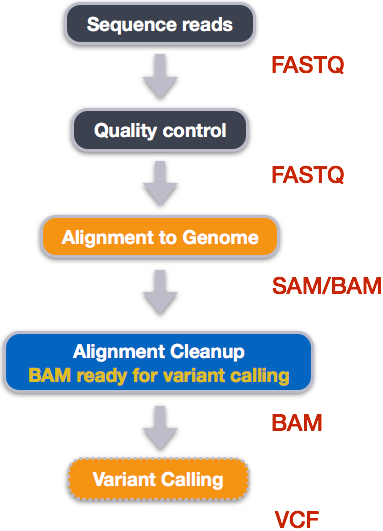
\includegraphics{images/pipeline.png}

\begin{enumerate}
\def\labelenumi{\arabic{enumi}.}
\item
  Quality control - Assessing quality
\item
  Quality control - Trimming and/or filtering reads (if necessary)
\item
  Align reads to reference genome
\item
  Perform post-alignment clean-up
\item
  Variant calling
\end{enumerate}

These workflows in bioinformatics adopt a plug-and-play approach in that
the output of one tool can be easily used as input to another tool
without any extensive configuration. Having standards for data formats
is what makes this feasible. Standards ensure that data is stored in a
way that is generally accepted and agreed upon within the community. The
tools that are used to analyze data at different stages of the workflow
are therefore built under the assumption that the data will be provided
in a specific format.

\hypertarget{get-the-data}{%
\section{Get the data}\label{get-the-data}}

Often times, the first step in a bioinformatic workflow is getting the
data you want to work with onto a computer where you can work with it.
If you have outsourced sequencing of your data, the sequencing center
will usually provide you with a link that you can use to download your
data. Today we will be working with publicly available sequencing data.

We are studying a population of \emph{Escherichia coli} (designated
Ara-3), which were propagated for more than 50,000 generations in a
glucose-limited minimal medium. We will be working with three samples
from this experiment, one from 5,000 generations, one from 15,000
generations, and one from 50,000 generations. The population changed
substantially during the course of the experiment, and we will be
exploring how with our variant calling workflow.

The data are paired-end, so we will download two files for each sample.
We will use the \href{https://www.ebi.ac.uk/ena}{European Nucleotide
Archive} to get our data. The ENA ``provides a comprehensive record of
the world's nucleotide sequencing information, covering raw sequencing
data, sequence assembly information and functional annotation.'' The ENA
also provides sequencing data in the fastq format, an important format
for sequencing reads that we will be learning about today.

\hypertarget{copy-directory-containing-data-on-the-hpc}{%
\subsection{Copy directory containing data on the
HPC}\label{copy-directory-containing-data-on-the-hpc}}

Using the terminal, you can access the remote server using the
\texttt{ssh} command (use your username)

\begin{Shaded}
\begin{Highlighting}[]
\ExtensionTok{$}\NormalTok{ ssh }\PreprocessorTok{[}\SpecialStringTok{username}\PreprocessorTok{]}\NormalTok{@hpc.tsl.ac.uk}
\end{Highlighting}
\end{Shaded}

Now that you are logged in on the server, we must start an
\texttt{interactive} session.

\begin{Shaded}
\begin{Highlighting}[]
\ExtensionTok{$}\NormalTok{ interactive}
\end{Highlighting}
\end{Shaded}

Copy the directory containing the dataset to your home directory.

\begin{Shaded}
\begin{Highlighting}[]
\ExtensionTok{$}\NormalTok{ cp }\AttributeTok{{-}r}\NormalTok{ /tsl/data/dc\_workshop/ \textasciitilde{}}
\end{Highlighting}
\end{Shaded}

Now you can access the directory that now should contain the fastq
files.

\begin{Shaded}
\begin{Highlighting}[]
\ExtensionTok{$}\NormalTok{ cd \textasciitilde{}/dc\_workshop/data/untrimmed\_fastq}
\end{Highlighting}
\end{Shaded}

The data comes in a compressed format, which is why there is a
\texttt{.gz} at the end of the file names. This makes it faster to
transfer, and allows it to take up less space on our computer. Let's
unzip one of the files so that we can look at the fastq format.

\begin{Shaded}
\begin{Highlighting}[]
\ExtensionTok{$}\NormalTok{ gunzip SRR2584863\_1.fastq.gz}
\end{Highlighting}
\end{Shaded}

It takes a few seconds.

\hypertarget{quality-control}{%
\section{Quality control}\label{quality-control}}

\hypertarget{details-on-the-fastq-format}{%
\subsection{Details on the FASTQ
format}\label{details-on-the-fastq-format}}

Although it looks complicated (and it is), we can understand the
\href{https://en.wikipedia.org/wiki/FASTQ_format}{fastq} format with a
little decoding. Some rules about the format include\ldots{}

\begin{longtable}[]{@{}
  >{\raggedright\arraybackslash}p{(\columnwidth - 2\tabcolsep) * \real{0.2778}}
  >{\raggedright\arraybackslash}p{(\columnwidth - 2\tabcolsep) * \real{0.7222}}@{}}
\toprule\noalign{}
\begin{minipage}[b]{\linewidth}\raggedright
Line
\end{minipage} & \begin{minipage}[b]{\linewidth}\raggedright
Description
\end{minipage} \\
\midrule\noalign{}
\endhead
\bottomrule\noalign{}
\endlastfoot
1 & Always begins with `@' and then information about the read \\
2 & The actual DNA sequence \\
3 & Always begins with a `+' and sometimes the same info in line 1 \\
4 & Has a string of characters which represent the quality scores; must
have same number of characters as line 2 \\
\end{longtable}

We can view the first complete read in one of the files our data set by
using \texttt{head} to look at the first four lines.

\begin{Shaded}
\begin{Highlighting}[]
\ExtensionTok{$}\NormalTok{ head }\AttributeTok{{-}n}\NormalTok{ 4 SRR2584863\_1.fastq}
\ExtensionTok{@SRR2584863.1}\NormalTok{ HWI{-}ST957:244:H73TDADXX:1:1101:4712:2181/1}
\ExtensionTok{TTCACATCCTGACCATTCAGTTGAGCAAAATAGTTCTTCAGTGCCTGTTTAACCGAGTCACGCAGGGGTTTTTGGGTTACCTGATCCTGAGAGTTAACGGTAGAAACGGTCAGTACGTCAGAATTTACGCGTTGTTCGAACATAGTTCTG}
\ExtensionTok{+}
\ExtensionTok{CCCFFFFFGHHHHJIJJJJIJJJIIJJJJIIIJJGFIIIJEDDFEGGJIFHHJIJJDECCGGEGIIJFHFFFACD:BBBDDACCCCAA@@CA@C}\OperatorTok{\textgreater{}}\NormalTok{C3}\OperatorTok{\textgreater{}}\NormalTok{@5}\ErrorTok{(}\ExtensionTok{8}\OperatorTok{\&\textgreater{}}\NormalTok{C:9}\PreprocessorTok{?}\NormalTok{8+89}\OperatorTok{\textless{}}\NormalTok{4}\ErrorTok{(}\ExtensionTok{:83825C}\ErrorTok{(}\ExtensionTok{:A\#\#\#\#\#\#\#\#\#\#\#\#\#\#\#\#\#\#\#\#\#\#\#\#\#}
\end{Highlighting}
\end{Shaded}

Line 4 shows the quality for each nucleotide in the read. Quality is
interpreted as the probability of an incorrect base call (e.g.~1 in 10)
or, equivalently, the base call accuracy (e.g.~90\%). To make it
possible to line up each individual nucleotide with its quality score,
the numerical score is converted into a code where each individual
character represents the numerical quality score for an individual
nucleotide. For example, in the line above, the quality score line is:

\begin{Shaded}
\begin{Highlighting}[]
\ExtensionTok{CCCFFFFFGHHHHJIJJJJIJJJIIJJJJIIIJJGFIIIJEDDFEGGJIFHHJIJJDECCGGEGIIJFHFFFACD:BBBDDACCCCAA@@CA@C}\OperatorTok{\textgreater{}}\NormalTok{C3}\OperatorTok{\textgreater{}}\NormalTok{@5}\ErrorTok{(}\ExtensionTok{8}\OperatorTok{\&\textgreater{}}\NormalTok{C:9}\PreprocessorTok{?}\NormalTok{8+89}\OperatorTok{\textless{}}\NormalTok{4}\ErrorTok{(}\ExtensionTok{:83825C}\ErrorTok{(}\ExtensionTok{:A\#\#\#\#\#\#\#\#\#\#\#\#\#\#\#\#\#\#\#\#\#\#\#\#\#}
\end{Highlighting}
\end{Shaded}

The numerical value assigned to each of these characters depends on the
sequencing platform that generated the reads. The sequencing machine
used to generate our data uses the standard Sanger quality PHRED score
encoding, using Illumina version 1.8 onwards. Each character is assigned
a quality score between 0 and 41 as shown in the chart below.

\begin{Shaded}
\begin{Highlighting}[]
\ExtensionTok{Quality}\NormalTok{ encoding: !}\StringTok{"\#$\%\&\textquotesingle{}()*+,{-}./0123456789:;\textless{}=\textgreater{}?@ABCDEFGHIJ}
\StringTok{                   |         |         |         |         |}
\StringTok{Quality score:    01........11........21........31........41}
\end{Highlighting}
\end{Shaded}

Each quality score represents the probability that the corresponding
nucleotide call is incorrect. This quality score is logarithmically
based, so a quality score of 10 reflects a base call accuracy of 90\%,
but a quality score of 20 reflects a base call accuracy of 99\%. These
probability values are the results from the base calling algorithm and
depend on how much signal was captured for the base incorporation.

Looking back at our read:

\begin{Shaded}
\begin{Highlighting}[]
\ExtensionTok{@SRR2584863.1}\NormalTok{ HWI{-}ST957:244:H73TDADXX:1:1101:4712:2181/1}
\ExtensionTok{TTCACATCCTGACCATTCAGTTGAGCAAAATAGTTCTTCAGTGCCTGTTTAACCGAGTCACGCAGGGGTTTTTGGGTTACCTGATCCTGAGAGTTAACGGTAGAAACGGTCAGTACGTCAGAATTTACGCGTTGTTCGAACATAGTTCTG}
\ExtensionTok{+}
\ExtensionTok{CCCFFFFFGHHHHJIJJJJIJJJIIJJJJIIIJJGFIIIJEDDFEGGJIFHHJIJJDECCGGEGIIJFHFFFACD:BBBDDACCCCAA@@CA@C}\OperatorTok{\textgreater{}}\NormalTok{C3}\OperatorTok{\textgreater{}}\NormalTok{@5}\ErrorTok{(}\ExtensionTok{8}\OperatorTok{\&\textgreater{}}\NormalTok{C:9}\PreprocessorTok{?}\NormalTok{8+89}\OperatorTok{\textless{}}\NormalTok{4}\ErrorTok{(}\ExtensionTok{:83825C}\ErrorTok{(}\ExtensionTok{:A\#\#\#\#\#\#\#\#\#\#\#\#\#\#\#\#\#\#\#\#\#\#\#\#\#}
\end{Highlighting}
\end{Shaded}

We can now see that there is a range of quality scores, but that the end
of the sequence is very poor (\texttt{\#} = a quality score of 2).

\begin{tcolorbox}[enhanced jigsaw, toptitle=1mm, breakable, bottomrule=.15mm, colback=white, toprule=.15mm, opacityback=0, bottomtitle=1mm, coltitle=black, opacitybacktitle=0.6, rightrule=.15mm, colframe=quarto-callout-caution-color-frame, titlerule=0mm, colbacktitle=quarto-callout-caution-color!10!white, title={Exercise}, left=2mm, leftrule=.75mm, arc=.35mm]

What is the last read in the \texttt{SRR2584863\_1.fastq} file? How
confident are you in this read?

\end{tcolorbox}

\begin{tcolorbox}[enhanced jigsaw, toptitle=1mm, breakable, bottomrule=.15mm, colback=white, toprule=.15mm, opacityback=0, bottomtitle=1mm, coltitle=black, opacitybacktitle=0.6, rightrule=.15mm, colframe=quarto-callout-caution-color-frame, titlerule=0mm, colbacktitle=quarto-callout-caution-color!10!white, title={Solution}, left=2mm, leftrule=.75mm, arc=.35mm]

\begin{Shaded}
\begin{Highlighting}[]
\ExtensionTok{$}\NormalTok{ tail }\AttributeTok{{-}n}\NormalTok{ 4 SRR2584863\_1.fastq}
\ExtensionTok{@SRR2584863.1553259}\NormalTok{ HWI{-}ST957:245:H73R4ADXX:2:2216:21048:100894/1}
\ExtensionTok{CTGCAATACCACGCTGATCTTTCACATGATGTAAGAAAAGTGGGATCAGCAAACCGGGTGCTGCTGTGGCTAGTTGCAGCAAACCATGCAGTGAACCCGCCTGTGCTTCGCTATAGCCGTGACTGATGAGGATCGCCGGAAGCCAGCCAA}
\ExtensionTok{+}
\ExtensionTok{CCCFFFFFHHHHGJJJJJJJJJHGIJJJIJJJJIJJJJIIIIJJJJJJJJJJJJJIIJJJHHHHHFFFFFEEEEEDDDDDDDDDDDDDDDDDCDEDDBDBDDBDDDDDDDDDBDEEDDDD7@BDDDDDD}\OperatorTok{\textgreater{}}\NormalTok{AA}\OperatorTok{\textgreater{}}\PreprocessorTok{?}\NormalTok{B}\PreprocessorTok{?}\OperatorTok{\textless{}}\NormalTok{@BDD@BDC}\PreprocessorTok{?}\NormalTok{BDA}\PreprocessorTok{?}
\end{Highlighting}
\end{Shaded}

This read has more consistent quality at its end than the first read
that we looked at, but still has a range of quality scores, most of them
high. We will look at variations in position-based quality in just a
moment.

\end{tcolorbox}

At this point, let's load the relevant tools that are already installed
on the server:

\begin{Shaded}
\begin{Highlighting}[]
\ExtensionTok{$}\NormalTok{ source package /nbi/software/production/bin/fastqc{-}0.11.8}
\ExtensionTok{loaded}\NormalTok{ /nbi/software/production/bin/fastqc{-}0.11.8}
\end{Highlighting}
\end{Shaded}

One way to validate if the correct software is loaded and ready to work
with is to check the software's manual:

\begin{Shaded}
\begin{Highlighting}[]
\ExtensionTok{$}\NormalTok{ fastqc }\AttributeTok{{-}h}
\end{Highlighting}
\end{Shaded}

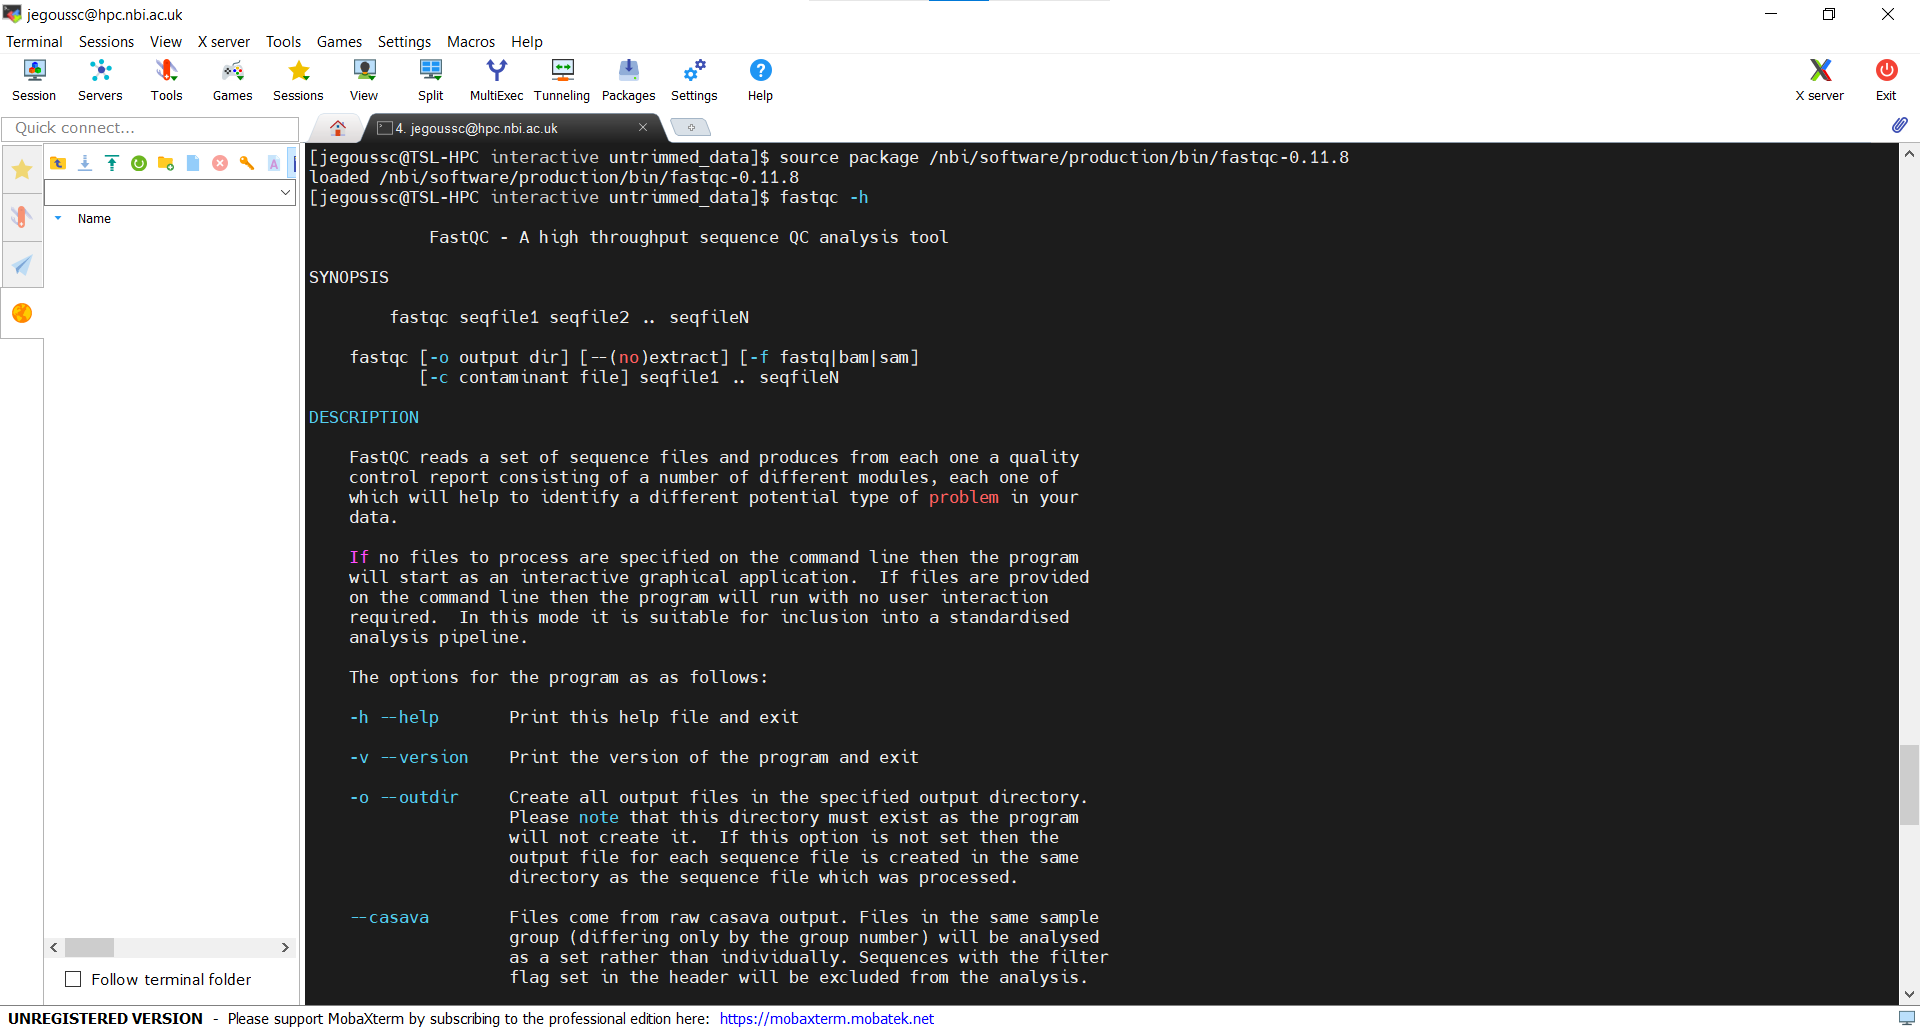
\includegraphics{images/fastqc-help.png}

If FastQC is not installed, you will get an error message:

\begin{Shaded}
\begin{Highlighting}[]
\ExtensionTok{$}\NormalTok{ fastqc }\AttributeTok{{-}h}
\ExtensionTok{The}\NormalTok{ program }\StringTok{\textquotesingle{}fastqc\textquotesingle{}}\NormalTok{ is currently not installed. You can install it by typing:}
\FunctionTok{sudo}\NormalTok{ apt{-}get install fastqc}
\end{Highlighting}
\end{Shaded}

If this happens check with your instructor before trying to install it.

\hypertarget{assessing-read-quality-with-fastqc}{%
\subsection{Assessing read quality with
FastQC}\label{assessing-read-quality-with-fastqc}}

In real life, you will not be assessing the quality of your reads by
visually inspecting your FASTQ files. Rather, you will be using a
software program to assess read quality and filter out poor quality
reads. We will first use a program called
\href{http://www.bioinformatics.babraham.ac.uk/projects/fastqc/}{FastQC}
(\textbf{andrews2010fastqcto?}) visualize the quality of our reads.
Later in our workflow, we will use another program to filter out poor
quality reads.

FastQC has a number of features which can give you a quick impression of
any problems your data may have, so you can take these issues into
consideration before moving forward with your analyses. Rather than
looking at quality scores for each individual read, FastQC looks at
quality collectively across all reads within a sample. The image below
shows one FastQC-generated plot that indicates a very high quality
sample:

\begin{figure}

{\centering 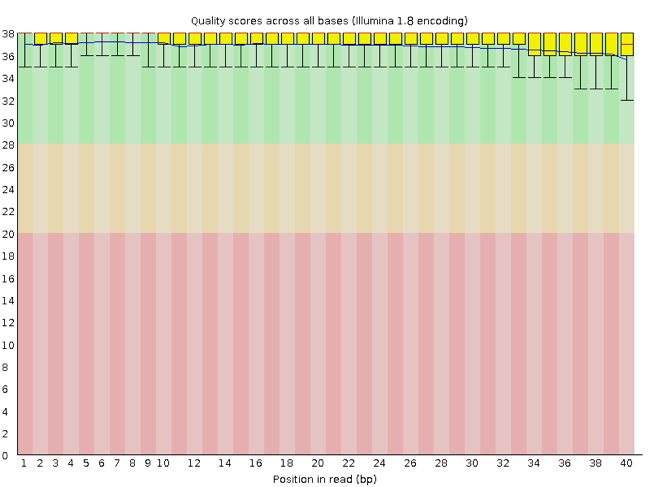
\includegraphics{images/fastqc-good.png}

}

\caption{good\_quality}

\end{figure}

The x-axis displays the base position in the read, and the y-axis shows
quality scores. In this example, the sample contains reads that are 40
bp long. This is much shorter than the reads we are working with in our
workflow. For each position, there is a box-and-whisker plot showing the
distribution of quality scores for all reads at that position. The
horizontal red line indicates the median quality score and the yellow
box shows the 1st to 3rd quartile range. This means that 50\% of reads
have a quality score that falls within the range of the yellow box at
that position. The whiskers show the absolute range, which covers the
lowest (0th quartile) to highest (4th quartile) values.

For each position in this sample, the quality values do not drop much
lower than 32. This is a high quality score. The plot background is also
color-coded to identify good (green), acceptable (yellow), and bad (red)
quality scores.

Now let's take a look at a quality plot on the other end of the
spectrum.

\begin{figure}

{\centering 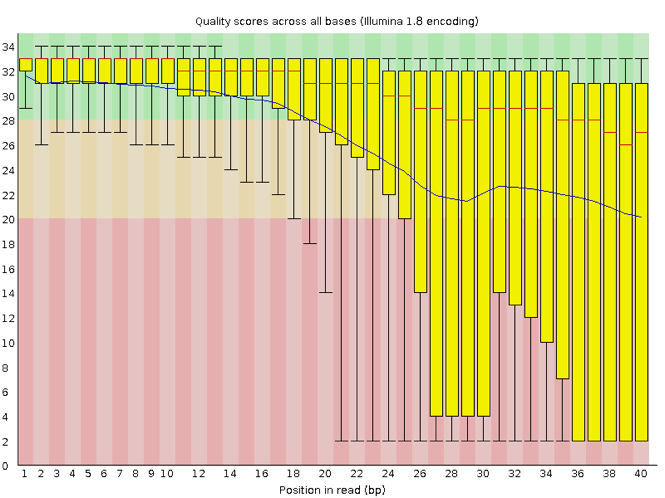
\includegraphics{images/fastqc-bad.png}

}

\caption{bad\_quality}

\end{figure}

Here, we see positions within the read in which the boxes span a much
wider range. Also, quality scores drop quite low into the ``bad'' range,
particularly on the tail end of the reads. The FastQC tool produces
several other diagnostic plots to assess sample quality, in addition to
the one plotted above.

\hypertarget{running-fastqc}{%
\subsection{Running FastQC}\label{running-fastqc}}

We will now assess the quality of the reads that we downloaded. First,
make sure you are still in the \texttt{untrimmed\_fastq} directory

\begin{Shaded}
\begin{Highlighting}[]
\BuiltInTok{cd}\NormalTok{ \textasciitilde{}/dc\_workshop/data/untrimmed\_fastq/}
\end{Highlighting}
\end{Shaded}

\begin{tcolorbox}[enhanced jigsaw, toptitle=1mm, breakable, bottomrule=.15mm, colback=white, toprule=.15mm, opacityback=0, bottomtitle=1mm, coltitle=black, opacitybacktitle=0.6, rightrule=.15mm, colframe=quarto-callout-caution-color-frame, titlerule=0mm, colbacktitle=quarto-callout-caution-color!10!white, title={Exercise}, left=2mm, leftrule=.75mm, arc=.35mm]

How big are the files? (Hint: Look at the options for the ls command to
see how to show file sizes.)

\end{tcolorbox}

\begin{tcolorbox}[enhanced jigsaw, toptitle=1mm, breakable, bottomrule=.15mm, colback=white, toprule=.15mm, opacityback=0, bottomtitle=1mm, coltitle=black, opacitybacktitle=0.6, rightrule=.15mm, colframe=quarto-callout-caution-color-frame, titlerule=0mm, colbacktitle=quarto-callout-caution-color!10!white, title={Solution}, left=2mm, leftrule=.75mm, arc=.35mm]

\begin{Shaded}
\begin{Highlighting}[]
\ExtensionTok{$}\NormalTok{ ls }\AttributeTok{{-}l} \AttributeTok{{-}h}
\ExtensionTok{{-}rwx{-}{-}{-}{-}{-}{-}}\NormalTok{ 1 }\PreprocessorTok{[}\SpecialStringTok{username}\PreprocessorTok{]}\NormalTok{ TSL\_20 545M Aug 11 11:02 SRR2584863\_1.fastq}
\ExtensionTok{{-}rwx{-}{-}{-}{-}{-}{-}}\NormalTok{ 1 }\PreprocessorTok{[}\SpecialStringTok{username}\PreprocessorTok{]}\NormalTok{ TSL\_20 183M Aug 11 11:03 SRR2584863\_2.fastq.gz}
\ExtensionTok{{-}rwx{-}{-}{-}{-}{-}{-}}\NormalTok{ 1 }\PreprocessorTok{[}\SpecialStringTok{username}\PreprocessorTok{]}\NormalTok{ TSL\_20 309M Aug 11 11:04 SRR2584866\_1.fastq.gz}
\ExtensionTok{{-}rwx{-}{-}{-}{-}{-}{-}}\NormalTok{ 1 }\PreprocessorTok{[}\SpecialStringTok{username}\PreprocessorTok{]}\NormalTok{ TSL\_20 296M Aug 11 11:07 SRR2584866\_2.fastq.gz}
\ExtensionTok{{-}rwx{-}{-}{-}{-}{-}{-}}\NormalTok{ 1 }\PreprocessorTok{[}\SpecialStringTok{username}\PreprocessorTok{]}\NormalTok{ TSL\_20 124M Aug 11 11:00 SRR2589044\_1.fastq.gz}
\ExtensionTok{{-}rwx{-}{-}{-}{-}{-}{-}}\NormalTok{ 1 }\PreprocessorTok{[}\SpecialStringTok{username}\PreprocessorTok{]}\NormalTok{ TSL\_20 128M Aug 11 11:01 SRR2589044\_2.fastq.gz}
\end{Highlighting}
\end{Shaded}

There are six FASTQ files ranging from 124M (124MB) to 545M.

\end{tcolorbox}

FastQC can accept multiple file names as input, and on both zipped and
unzipped files, so we can use the *.fastq* wildcard to run FastQC on all
of the FASTQ files in this directory.

\begin{Shaded}
\begin{Highlighting}[]
\ExtensionTok{$}\NormalTok{ fastqc }\PreprocessorTok{*}\NormalTok{.fastq}\PreprocessorTok{*}
\end{Highlighting}
\end{Shaded}

You will see an automatically updating output message telling you the
progress of the analysis. It will start like this:

\begin{verbatim}
Started analysis of SRR2584863_1.fastq
Approx 5% complete for SRR2584863_1.fastq
Approx 10% complete for SRR2584863_1.fastq
Approx 15% complete for SRR2584863_1.fastq
Approx 20% complete for SRR2584863_1.fastq
Approx 25% complete for SRR2584863_1.fastq
Approx 30% complete for SRR2584863_1.fastq
Approx 35% complete for SRR2584863_1.fastq
Approx 40% complete for SRR2584863_1.fastq
Approx 45% complete for SRR2584863_1.fastq
\end{verbatim}

In total, it should take about five minutes for FastQC to run on all six
of our FASTQ files. When the analysis completes, your prompt will
return. So your screen will look something like this:

\begin{verbatim}
Approx 80% complete for SRR2589044_2.fastq.gz
Approx 85% complete for SRR2589044_2.fastq.gz
Approx 90% complete for SRR2589044_2.fastq.gz
Approx 95% complete for SRR2589044_2.fastq.gz
Analysis complete for SRR2589044_2.fastq.gz
$
\end{verbatim}

The FastQC program has created several new files within our
\texttt{data/untrimmed\_fastq/} directory.

\begin{Shaded}
\begin{Highlighting}[]
\ExtensionTok{$}\NormalTok{ ls}
\ExtensionTok{SRR2584863\_1.fastq}\NormalTok{        SRR2584866\_1\_fastqc.html  SRR2589044\_1\_fastqc.html}
\ExtensionTok{SRR2584863\_1\_fastqc.html}\NormalTok{  SRR2584866\_1\_fastqc.zip   SRR2589044\_1\_fastqc.zip}
\ExtensionTok{SRR2584863\_1\_fastqc.zip}\NormalTok{   SRR2584866\_1.fastq.gz     SRR2589044\_1.fastq.gz}
\ExtensionTok{SRR2584863\_2\_fastqc.html}\NormalTok{  SRR2584866\_2\_fastqc.html  SRR2589044\_2\_fastqc.html}
\ExtensionTok{SRR2584863\_2\_fastqc.zip}\NormalTok{   SRR2584866\_2\_fastqc.zip   SRR2589044\_2\_fastqc.zip}
\ExtensionTok{SRR2584863\_2.fastq.gz}\NormalTok{     SRR2584866\_2.fastq.gz     SRR2589044\_2.fastq.gz}
\end{Highlighting}
\end{Shaded}

For each input FASTQ file, FastQC has created a \texttt{.zip} file and a

\texttt{.html} file. The \texttt{.zip} file extension indicates that
this is actually a compressed set of multiple output files. We will be
working with these output files soon. The \texttt{.html} file is a
stable webpage displaying the summary report for each of our samples.

We want to keep our data files and our results files separate, so we
will move these output files into a new directory within our
\texttt{results/} directory.

\begin{Shaded}
\begin{Highlighting}[]
\ExtensionTok{$}\NormalTok{ mkdir }\AttributeTok{{-}p}\NormalTok{ \textasciitilde{}/dc\_workshop/results/fastqc\_untrimmed\_reads}
\ExtensionTok{$}\NormalTok{ mv }\PreprocessorTok{*}\NormalTok{.zip \textasciitilde{}/dc\_workshop/results/fastqc\_untrimmed\_reads/}
\ExtensionTok{$}\NormalTok{ mv }\PreprocessorTok{*}\NormalTok{.html \textasciitilde{}/dc\_workshop/results/fastqc\_untrimmed\_reads/}
\end{Highlighting}
\end{Shaded}

Now we can navigate into this results directory and do some closer
inspection of our output files.

\begin{Shaded}
\begin{Highlighting}[]
\ExtensionTok{$}\NormalTok{ cd \textasciitilde{}/dc\_workshop/results/fastqc\_untrimmed\_reads/}
\end{Highlighting}
\end{Shaded}

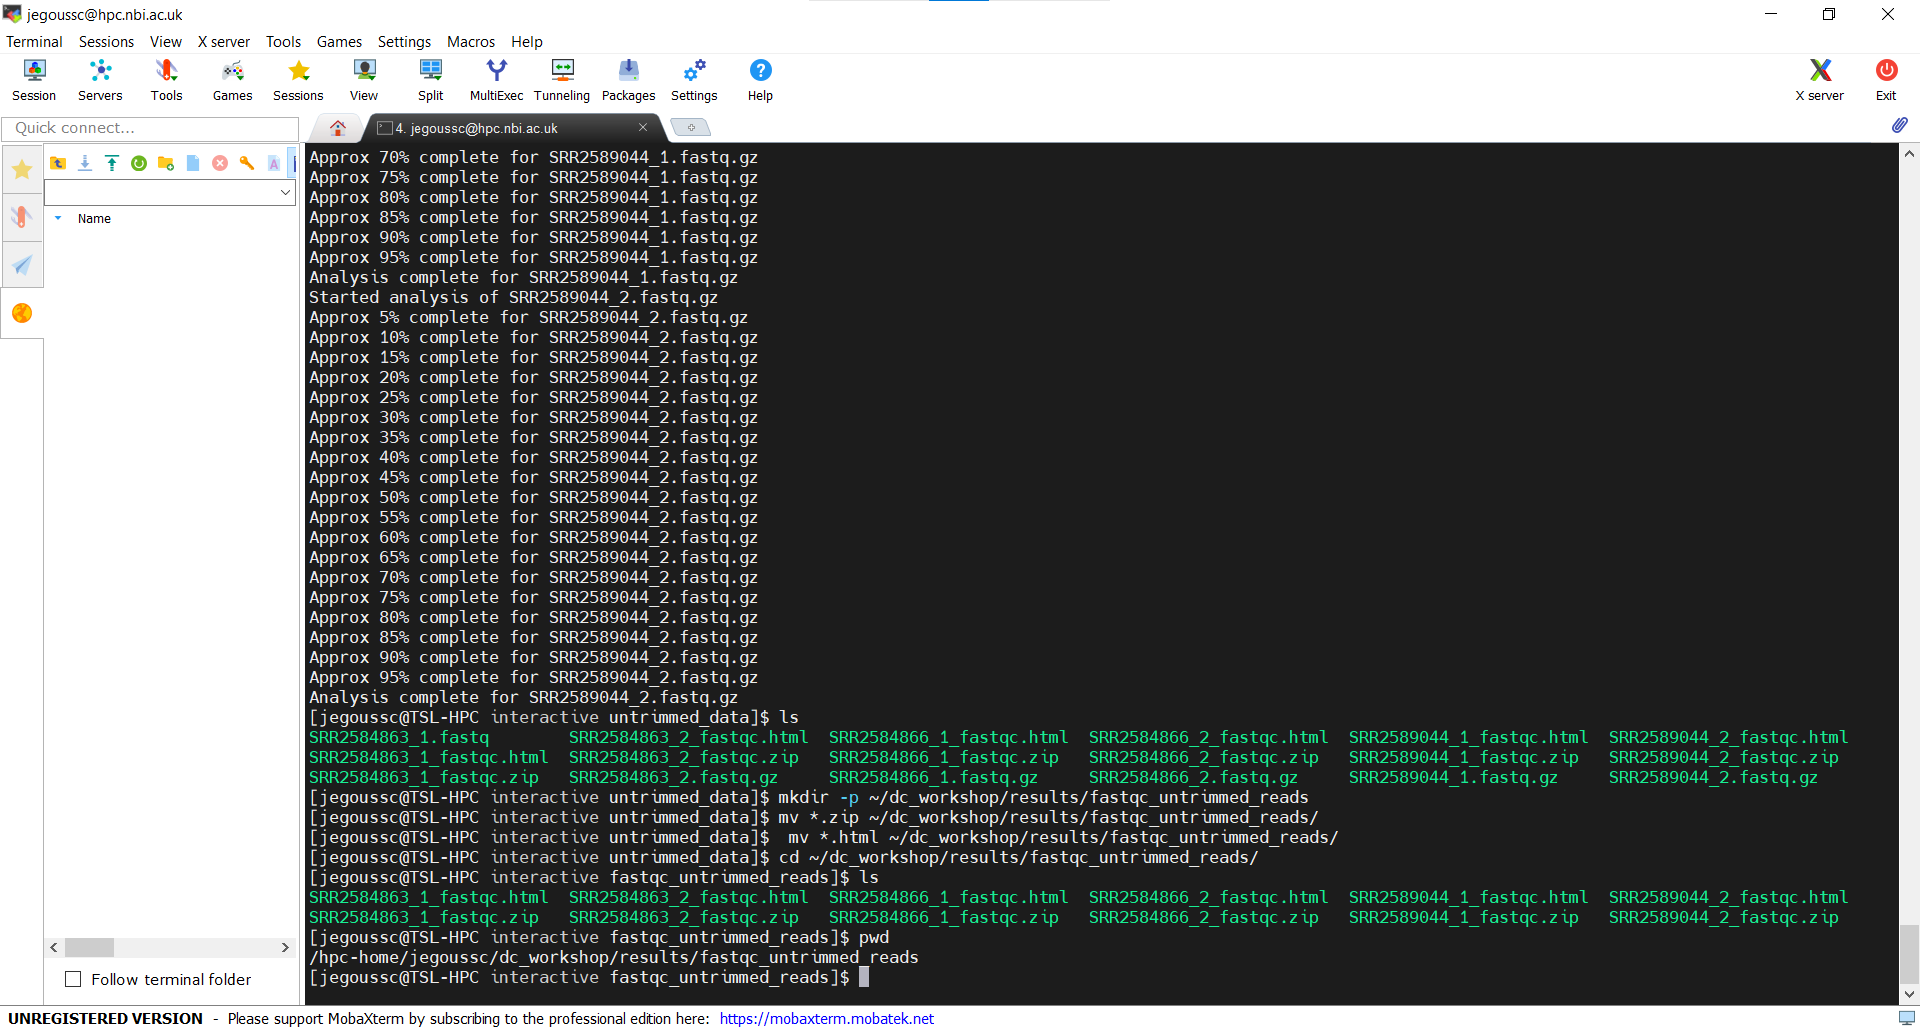
\includegraphics{images/fastqc-output.png}

\hypertarget{viewing-the-fastqc-results}{%
\subsection{Viewing the FastQC
results}\label{viewing-the-fastqc-results}}

If we were working on our local computers, we would be able to look at
each of these HTML files by opening them in a web browser.

However, these files are currently sitting on our remote server, where
our local computer can not see them. And, since we are only logging into
the server via the command line - it does not have any web browser setup
to display these files either.

So the easiest way to look at these webpage summary reports will be to
transfer them to our local computers (i.e.~your laptop).

To transfer a file from a remote server to our own machines, we will
simply use the Windows navigation system.

\begin{enumerate}
\def\labelenumi{\arabic{enumi}.}
\tightlist
\item
  From the Start Menu, select Run, then type
  \texttt{\textbackslash{}\textbackslash{}tsl-hpc-data\textbackslash{}HPC-Home}
\item
  You may need to toggle \texttt{Use\ different\ credentials} on or off
\end{enumerate}

A window with the directory showing the files in should pop up

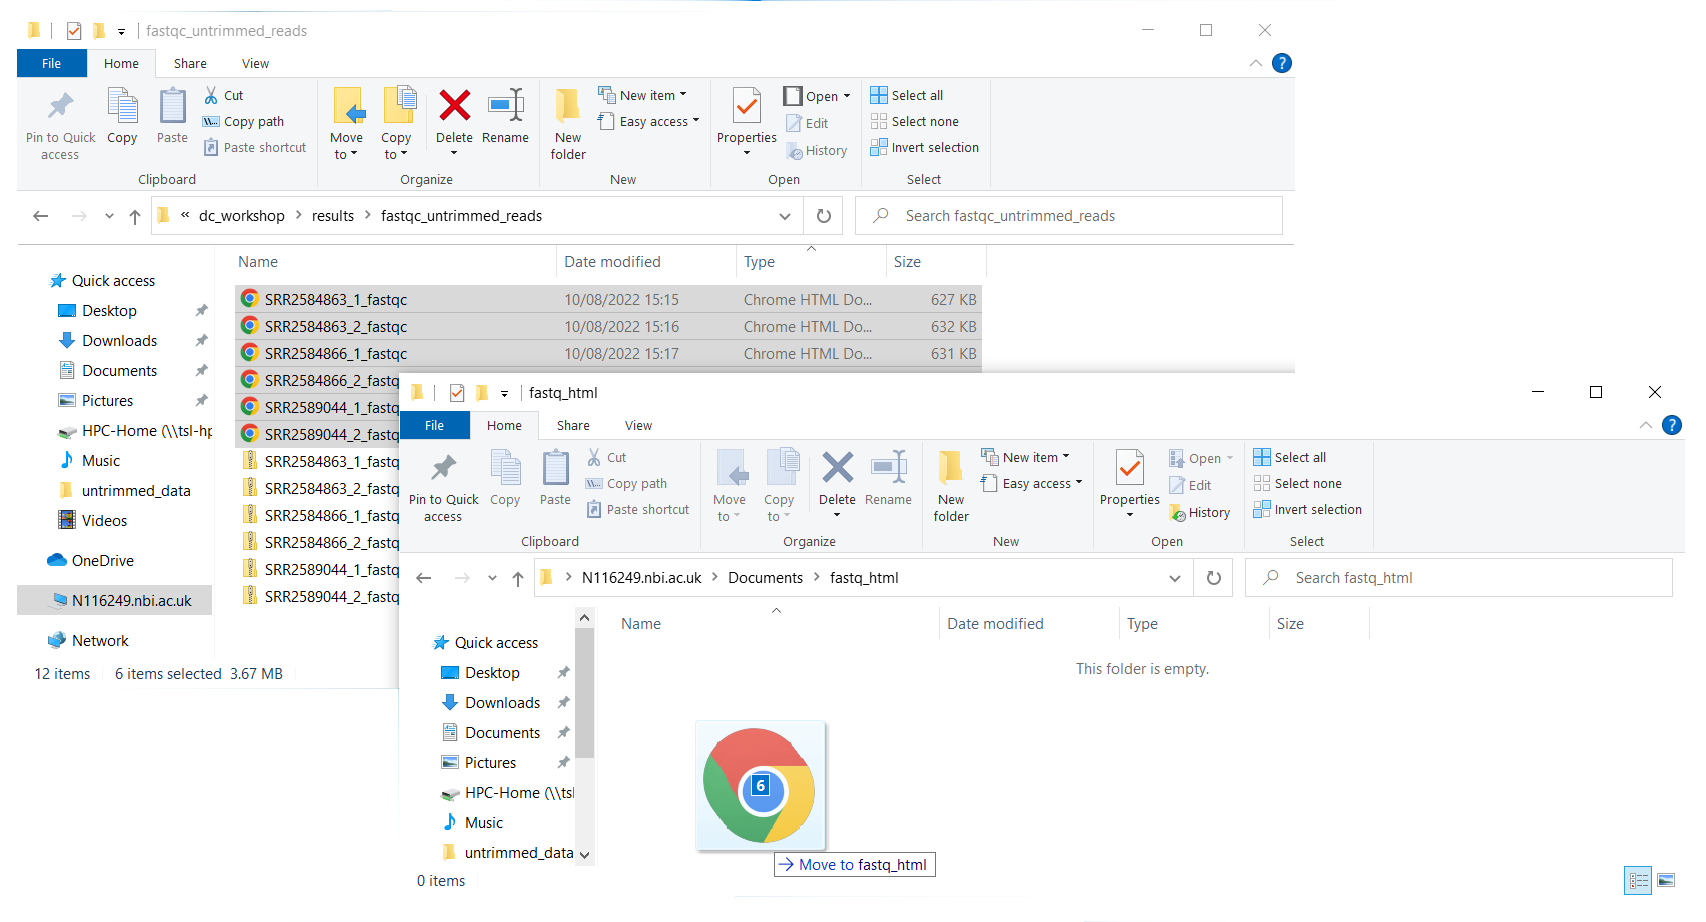
\includegraphics{images/transfer-results-to-local.png}

Now we can go to our new directory and open the 6 HTML files.

Depending on your system, you should be able to select and open them all
at once via a right click menu in your file browser.

\begin{tcolorbox}[enhanced jigsaw, toptitle=1mm, breakable, bottomrule=.15mm, colback=white, toprule=.15mm, opacityback=0, bottomtitle=1mm, coltitle=black, opacitybacktitle=0.6, rightrule=.15mm, colframe=quarto-callout-caution-color-frame, titlerule=0mm, colbacktitle=quarto-callout-caution-color!10!white, title={Exercise}, left=2mm, leftrule=.75mm, arc=.35mm]

Discuss your results with a neighbor. Which sample(s) looks the best in
terms of per base sequence quality? Which sample(s) look the worst?

\end{tcolorbox}

\begin{tcolorbox}[enhanced jigsaw, toptitle=1mm, breakable, bottomrule=.15mm, colback=white, toprule=.15mm, opacityback=0, bottomtitle=1mm, coltitle=black, opacitybacktitle=0.6, rightrule=.15mm, colframe=quarto-callout-caution-color-frame, titlerule=0mm, colbacktitle=quarto-callout-caution-color!10!white, title={Solution}, left=2mm, leftrule=.75mm, arc=.35mm]

All of the reads contain usable data, but the quality decreases toward
the end of the reads.

\end{tcolorbox}

\hypertarget{decoding-the-other-fastqc-outputs}{%
\subsection{\texorpdfstring{\textbf{Decoding the other FastQC
outputs}}{Decoding the other FastQC outputs}}\label{decoding-the-other-fastqc-outputs}}

We have now looked at quite a few ``Per base sequence quality'' FastQC
graphs, but there are nine other graphs that we have not talked about!
Below we have provided a brief overview of interpretations for each of
these plots. For more information, please see the FastQC documentation
\href{https://www.bioinformatics.babraham.ac.uk/projects/fastqc/Help/}{here}

\begin{itemize}
\item
  \href{https://www.bioinformatics.babraham.ac.uk/projects/fastqc/Help/3\%20Analysis\%20Modules/12\%20Per\%20Tile\%20Sequence\%20Quality.html}{\textbf{Per
  tile sequence quality}}: the machines that perform sequencing are
  divided into tiles. This plot displays patterns in base quality along
  these tiles. Consistently low scores are often found around the edges,
  but hot spots can also occur in the middle if an air bubble was
  introduced at some point during the run.
\item
  \href{https://www.bioinformatics.babraham.ac.uk/projects/fastqc/Help/3\%20Analysis\%20Modules/3\%20Per\%20Sequence\%20Quality\%20Scores.html}{\textbf{Per
  sequence quality scores}}: a density plot of quality for all reads at
  all positions. This plot shows what quality scores are most common.
\item
  \href{https://www.bioinformatics.babraham.ac.uk/projects/fastqc/Help/3\%20Analysis\%20Modules/4\%20Per\%20Base\%20Sequence\%20Content.html}{\textbf{Per
  base sequence content}}: plots the proportion of each base position
  over all of the reads. Typically, we expect to see each base roughly
  25\% of the time at each position, but this often fails at the
  beginning or end of the read due to quality or adapter content.
\item
  \href{https://www.bioinformatics.babraham.ac.uk/projects/fastqc/Help/3\%20Analysis\%20Modules/5\%20Per\%20Sequence\%20GC\%20Content.html}{\textbf{Per
  sequence GC content}}: a density plot of average GC content in each of
  the reads.
\item
  \href{https://www.bioinformatics.babraham.ac.uk/projects/fastqc/Help/3\%20Analysis\%20Modules/6\%20Per\%20Base\%20N\%20Content.html}{\textbf{Per
  base N content}}: the percent of times that `N' occurs at a position
  in all reads. If there is an increase at a particular position, this
  might indicate that something went wrong during sequencing.
\item
  \href{https://www.bioinformatics.babraham.ac.uk/projects/fastqc/Help/3\%20Analysis\%20Modules/7\%20Sequence\%20Length\%20Distribution.html}{\textbf{Sequence
  Length Distribution}}: the distribution of sequence lengths of all
  reads in the file. If the data is raw, there is often on sharp peak,
  however if the reads have been trimmed, there may be a distribution of
  shorter lengths.
\item
  \href{https://www.bioinformatics.babraham.ac.uk/projects/fastqc/Help/3\%20Analysis\%20Modules/8\%20Duplicate\%20Sequences.html}{\textbf{Sequence
  Duplication Levels}}: A distribution of duplicated sequences. In
  sequencing, we expect most reads to only occur once. If some sequences
  are occurring more than once, it might indicate enrichment bias
  (e.g.~from PCR). If the samples are high coverage (or RNA-seq or
  amplicon), this might not be true.
\item
  \href{https://www.bioinformatics.babraham.ac.uk/projects/fastqc/Help/3\%20Analysis\%20Modules/9\%20Overrepresented\%20Sequences.html}{\textbf{Overrepresented
  sequences}}: A list of sequences that occur more frequently than would
  be expected by chance.
\item
  \href{https://www.bioinformatics.babraham.ac.uk/projects/fastqc/Help/3\%20Analysis\%20Modules/10\%20Adapter\%20Content.html}{\textbf{Adapter
  Content}}: a graph indicating where adapater sequences occur in the
  reads.
\item
  \href{https://www.bioinformatics.babraham.ac.uk/projects/fastqc/Help/3\%20Analysis\%20Modules/11\%20Kmer\%20Content.html}{\textbf{K-mer
  Content}}: a graph showing any sequences which may show a positional
  bias within the reads.
\end{itemize}

\hypertarget{working-with-the-fastqc-text-output}{%
\subsection{Working with the FastQC text
output}\label{working-with-the-fastqc-text-output}}

Now that we have looked at our HTML reports to get a feel for the data,
let's look more closely at the other output files. Go back to the tab in
your terminal program that is connected to your interactive session on
the server and make sure you are in our results subdirectory.

\begin{Shaded}
\begin{Highlighting}[]
\ExtensionTok{$}\NormalTok{ cd \textasciitilde{}/dc\_workshop/results/fastqc\_untrimmed\_reads/}
\ExtensionTok{$}\NormalTok{ ls}
\ExtensionTok{SRR2584863\_1\_fastqc.html}\NormalTok{  SRR2584866\_1\_fastqc.html  SRR2589044\_1\_fastqc.html}
\ExtensionTok{SRR2584863\_1\_fastqc.zip}\NormalTok{   SRR2584866\_1\_fastqc.zip   SRR2589044\_1\_fastqc.zip}
\ExtensionTok{SRR2584863\_2\_fastqc.html}\NormalTok{  SRR2584866\_2\_fastqc.html  SRR2589044\_2\_fastqc.html}
\ExtensionTok{SRR2584863\_2\_fastqc.zip}\NormalTok{   SRR2584866\_2\_fastqc.zip   SRR2589044\_2\_fastqc.zip}
\end{Highlighting}
\end{Shaded}

Our \texttt{.zip} files are compressed files. They each contain multiple
different types of output files for a single input FASTQ file. To view
the contents of a \texttt{.zip} file, we can use the program
\texttt{unzip} to decompress these files. Let's try doing them all at
once using a wildcard.

\begin{Shaded}
\begin{Highlighting}[]
\ExtensionTok{$}\NormalTok{ unzip }\PreprocessorTok{*}\NormalTok{.zip}
\ExtensionTok{Archive:}\NormalTok{  SRR2584863\_1\_fastqc.zip}
\ExtensionTok{caution:}\NormalTok{ filename not matched:  SRR2584863\_2\_fastqc.zip}
\ExtensionTok{caution:}\NormalTok{ filename not matched:  SRR2584866\_1\_fastqc.zip}
\ExtensionTok{caution:}\NormalTok{ filename not matched:  SRR2584866\_2\_fastqc.zip}
\ExtensionTok{caution:}\NormalTok{ filename not matched:  SRR2589044\_1\_fastqc.zip}
\ExtensionTok{caution:}\NormalTok{ filename not matched:  SRR2589044\_2\_fastqc.zip}
\end{Highlighting}
\end{Shaded}

This did not work. We unzipped the first file and then got a warning
message for each of the other \texttt{.zip} files. This is because
\texttt{unzip} expects to get only one zip file as input. We could go
through and unzip each file one at a time, but this is very time
consuming and error-prone. Someday you may have 500 files to unzip!

A more efficient way is to use a \texttt{for} loop like we learned in
the Shell Genomics lesson to iterate through all of our \texttt{.zip}
files. Let's see what that looks like and then we will discuss what we
are doing with each line of our loop.

\begin{tcolorbox}[enhanced jigsaw, toptitle=1mm, breakable, bottomrule=.15mm, colback=white, toprule=.15mm, opacityback=0, bottomtitle=1mm, coltitle=black, opacitybacktitle=0.6, rightrule=.15mm, colframe=quarto-callout-warning-color-frame, titlerule=0mm, colbacktitle=quarto-callout-warning-color!10!white, title=\textcolor{quarto-callout-warning-color}{\faExclamationTriangle}\hspace{0.5em}{Warning}, left=2mm, leftrule=.75mm, arc=.35mm]

Do not copy-paste the four lines at once. You must type the \texttt{for}
loop line by line!

\end{tcolorbox}

\begin{Shaded}
\begin{Highlighting}[]
\ExtensionTok{$}\NormalTok{ for filename in }\PreprocessorTok{*}\NormalTok{.zip}
\OperatorTok{\textgreater{}}\NormalTok{ do}
\OperatorTok{\textgreater{}}\NormalTok{ unzip }\VariableTok{$filename}
\OperatorTok{\textgreater{}}\NormalTok{ done}
\end{Highlighting}
\end{Shaded}

In this example, the input is six filenames (one filename for each of
our \texttt{.zip} files). Each time the loop iterates, it will assign a
file name to the variable \texttt{filename} and run the \texttt{unzip}
command. The first time through the loop, \texttt{\$filename} is
\texttt{SRR2584863\_1\_fastqc.zip}. The interpreter runs the command
\texttt{unzip} on \texttt{SRR2584863\_1\_fastqc.zip}. For the second
iteration, \texttt{\$filename} becomes
\texttt{SRR2584863\_2\_fastqc.zip}. This time, the shell runs
\texttt{unzip} on \texttt{SRR2584863\_2\_fastqc.zip}. It then repeats
this process for the four other \texttt{.zip} files in our directory.

When we run our \texttt{for} loop, you will see output that starts like
this:

\begin{verbatim}
Archive:  SRR2589044_2_fastqc.zip
   creating: SRR2589044_2_fastqc/
   creating: SRR2589044_2_fastqc/Icons/
   creating: SRR2589044_2_fastqc/Images/
  inflating: SRR2589044_2_fastqc/Icons/fastqc_icon.png
  inflating: SRR2589044_2_fastqc/Icons/warning.png
  inflating: SRR2589044_2_fastqc/Icons/error.png
  inflating: SRR2589044_2_fastqc/Icons/tick.png
  inflating: SRR2589044_2_fastqc/summary.txt
  inflating: SRR2589044_2_fastqc/Images/per_base_quality.png
  inflating: SRR2589044_2_fastqc/Images/per_tile_quality.png
  inflating: SRR2589044_2_fastqc/Images/per_sequence_quality.png
  inflating: SRR2589044_2_fastqc/Images/per_base_sequence_content.png
  inflating: SRR2589044_2_fastqc/Images/per_sequence_gc_content.png
  inflating: SRR2589044_2_fastqc/Images/per_base_n_content.png
  inflating: SRR2589044_2_fastqc/Images/sequence_length_distribution.png
  inflating: SRR2589044_2_fastqc/Images/duplication_levels.png
  inflating: SRR2589044_2_fastqc/Images/adapter_content.png
  inflating: SRR2589044_2_fastqc/fastqc_report.html
  inflating: SRR2589044_2_fastqc/fastqc_data.txt
  inflating: SRR2589044_2_fastqc/fastqc.fo
\end{verbatim}

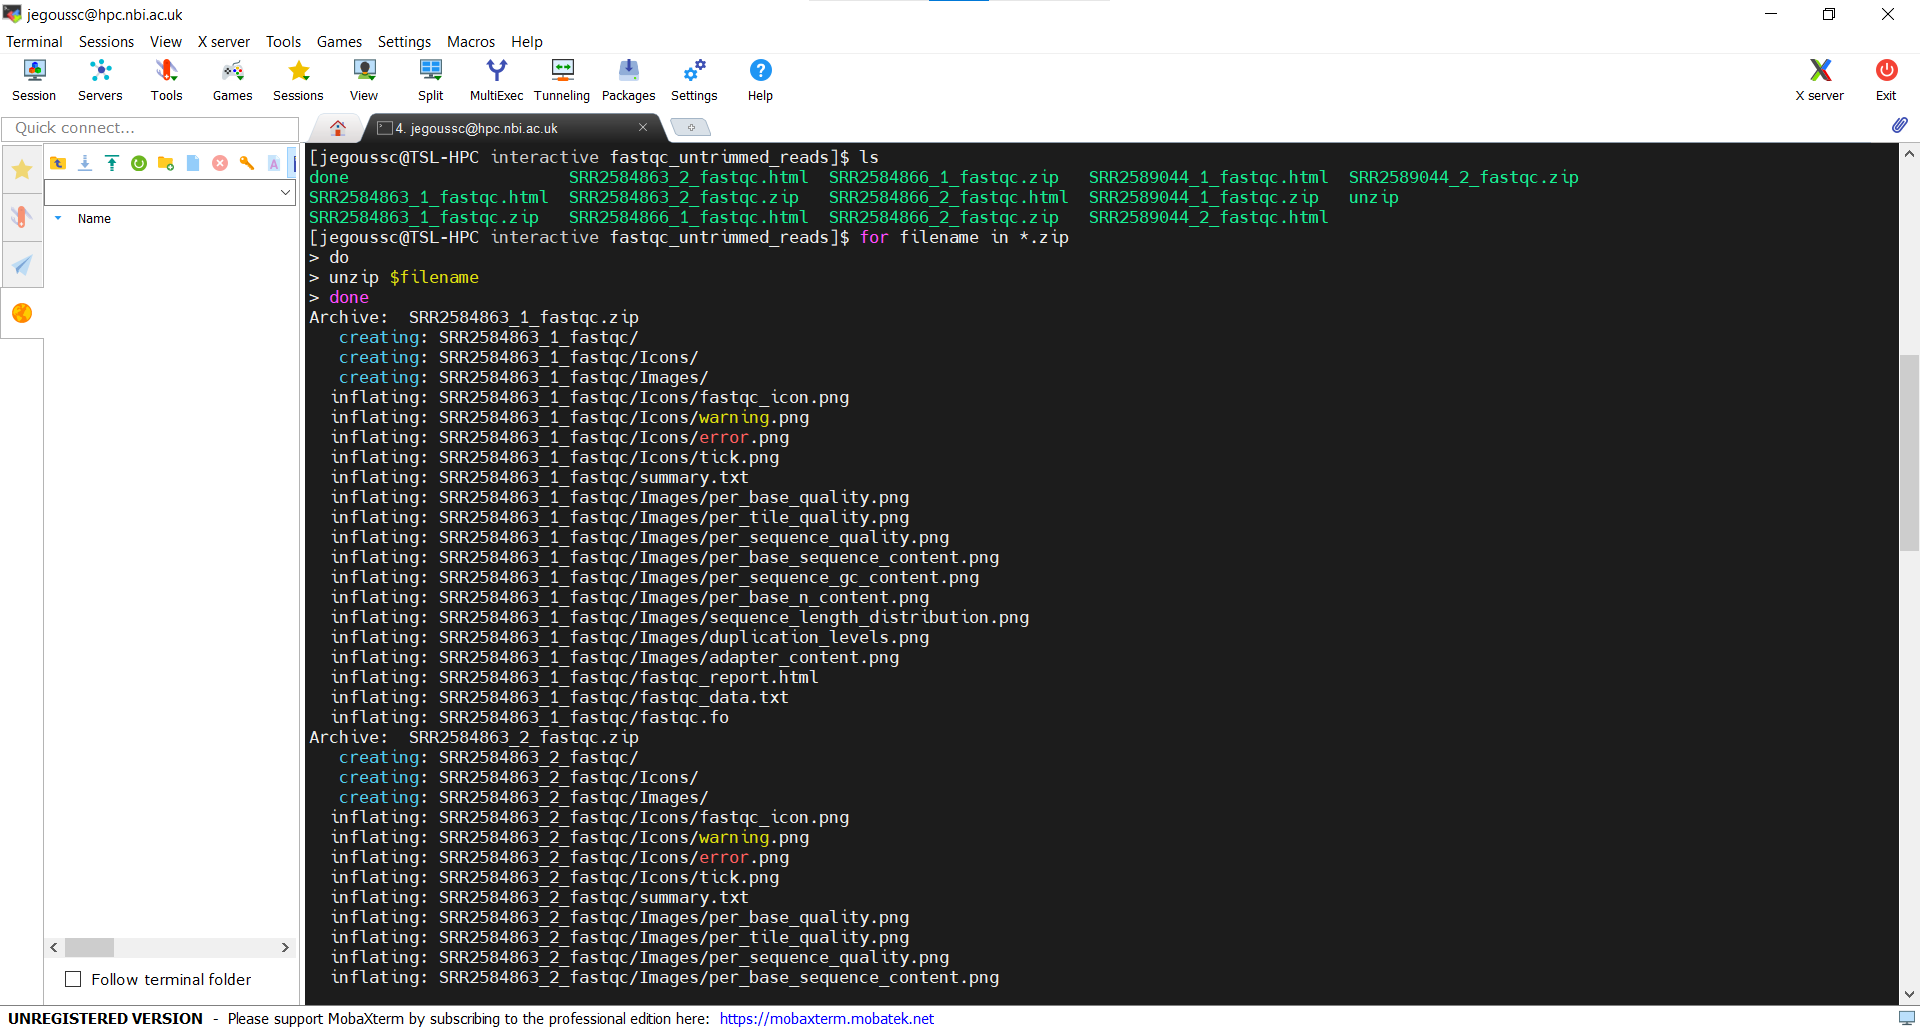
\includegraphics{images/unzip-fastqc-output-file.png}

The \texttt{unzip} program is decompressing the \texttt{.zip} files and
creating a new directory (with subdirectories) for each of our samples,
to store all of the different output that is produced by FastQC. There

are a lot of files here. The one we are going to focus on is the
\texttt{summary.txt} file.

If you list the files in our directory now you will see:

\begin{verbatim}
SRR2584863_1_fastqc       SRR2584866_1_fastqc       SRR2589044_1_fastqc
SRR2584863_1_fastqc.html  SRR2584866_1_fastqc.html  SRR2589044_1_fastqc.html
SRR2584863_1_fastqc.zip   SRR2584866_1_fastqc.zip   SRR2589044_1_fastqc.zip
SRR2584863_2_fastqc       SRR2584866_2_fastqc       SRR2589044_2_fastqc
SRR2584863_2_fastqc.html  SRR2584866_2_fastqc.html  SRR2589044_2_fastqc.html
SRR2584863_2_fastqc.zip   SRR2584866_2_fastqc.zip   SRR2589044_2_fastqc.zip
\end{verbatim}

The \texttt{.html} files and the uncompressed \texttt{.zip} files are
still present, but now we also have a new directory for each of our
samples. We can see for sure that it is a directory if we use the
\texttt{-F} flag for \texttt{ls}.

\begin{Shaded}
\begin{Highlighting}[]
\ExtensionTok{$}\NormalTok{ ls }\AttributeTok{{-}F}
\ExtensionTok{SRR2584863\_1\_fastqc/}\NormalTok{      SRR2584866\_1\_fastqc/      SRR2589044\_1\_fastqc/}
\ExtensionTok{SRR2584863\_1\_fastqc.html}\NormalTok{  SRR2584866\_1\_fastqc.html  SRR2589044\_1\_fastqc.html}
\ExtensionTok{SRR2584863\_1\_fastqc.zip}\NormalTok{   SRR2584866\_1\_fastqc.zip   SRR2589044\_1\_fastqc.zip}
\ExtensionTok{SRR2584863\_2\_fastqc/}\NormalTok{      SRR2584866\_2\_fastqc/      SRR2589044\_2\_fastqc/}
\ExtensionTok{SRR2584863\_2\_fastqc.html}\NormalTok{  SRR2584866\_2\_fastqc.html  SRR2589044\_2\_fastqc.html}
\ExtensionTok{SRR2584863\_2\_fastqc.zip}\NormalTok{   SRR2584866\_2\_fastqc.zip   SRR2589044\_2\_fastqc.zip}
\end{Highlighting}
\end{Shaded}

Let's see what files are present within one of these output directories.

\begin{Shaded}
\begin{Highlighting}[]
\ExtensionTok{$}\NormalTok{ ls }\AttributeTok{{-}F}\NormalTok{ SRR2584863\_1\_fastqc/}
\ExtensionTok{fastqc\_data.txt}\NormalTok{  fastqc.fo  fastqc\_report.html  Icons/  Images/  summary.txt}
\end{Highlighting}
\end{Shaded}

Use \texttt{less} to preview the \texttt{summary.txt} file for this
sample.

\begin{Shaded}
\begin{Highlighting}[]
\ExtensionTok{$}\NormalTok{ less SRR2584863\_1\_fastqc/summary.txt}

\ExtensionTok{PASS}\NormalTok{    Basic Statistics        SRR2584863\_1.fastq}
\ExtensionTok{PASS}\NormalTok{    Per base sequence quality       SRR2584863\_1.fastq}
\ExtensionTok{PASS}\NormalTok{    Per tile sequence quality       SRR2584863\_1.fastq}
\ExtensionTok{PASS}\NormalTok{    Per sequence quality scores     SRR2584863\_1.fastq}
\ExtensionTok{WARN}\NormalTok{    Per base sequence content       SRR2584863\_1.fastq}
\ExtensionTok{WARN}\NormalTok{    Per sequence GC content SRR2584863\_1.fastq}
\ExtensionTok{PASS}\NormalTok{    Per base N content      SRR2584863\_1.fastq}
\ExtensionTok{PASS}\NormalTok{    Sequence Length Distribution    SRR2584863\_1.fastq}
\ExtensionTok{PASS}\NormalTok{    Sequence Duplication Levels     SRR2584863\_1.fastq}
\ExtensionTok{PASS}\NormalTok{    Overrepresented sequences       SRR2584863\_1.fastq}
\ExtensionTok{WARN}\NormalTok{    Adapter Content SRR2584863\_1.fastq}
\end{Highlighting}
\end{Shaded}

The summary file gives us a list of tests that FastQC ran, and tells us
whether this sample passed, failed, or is borderline (\texttt{WARN}).
Remember, to quit from \texttt{less} you must type \texttt{q}.

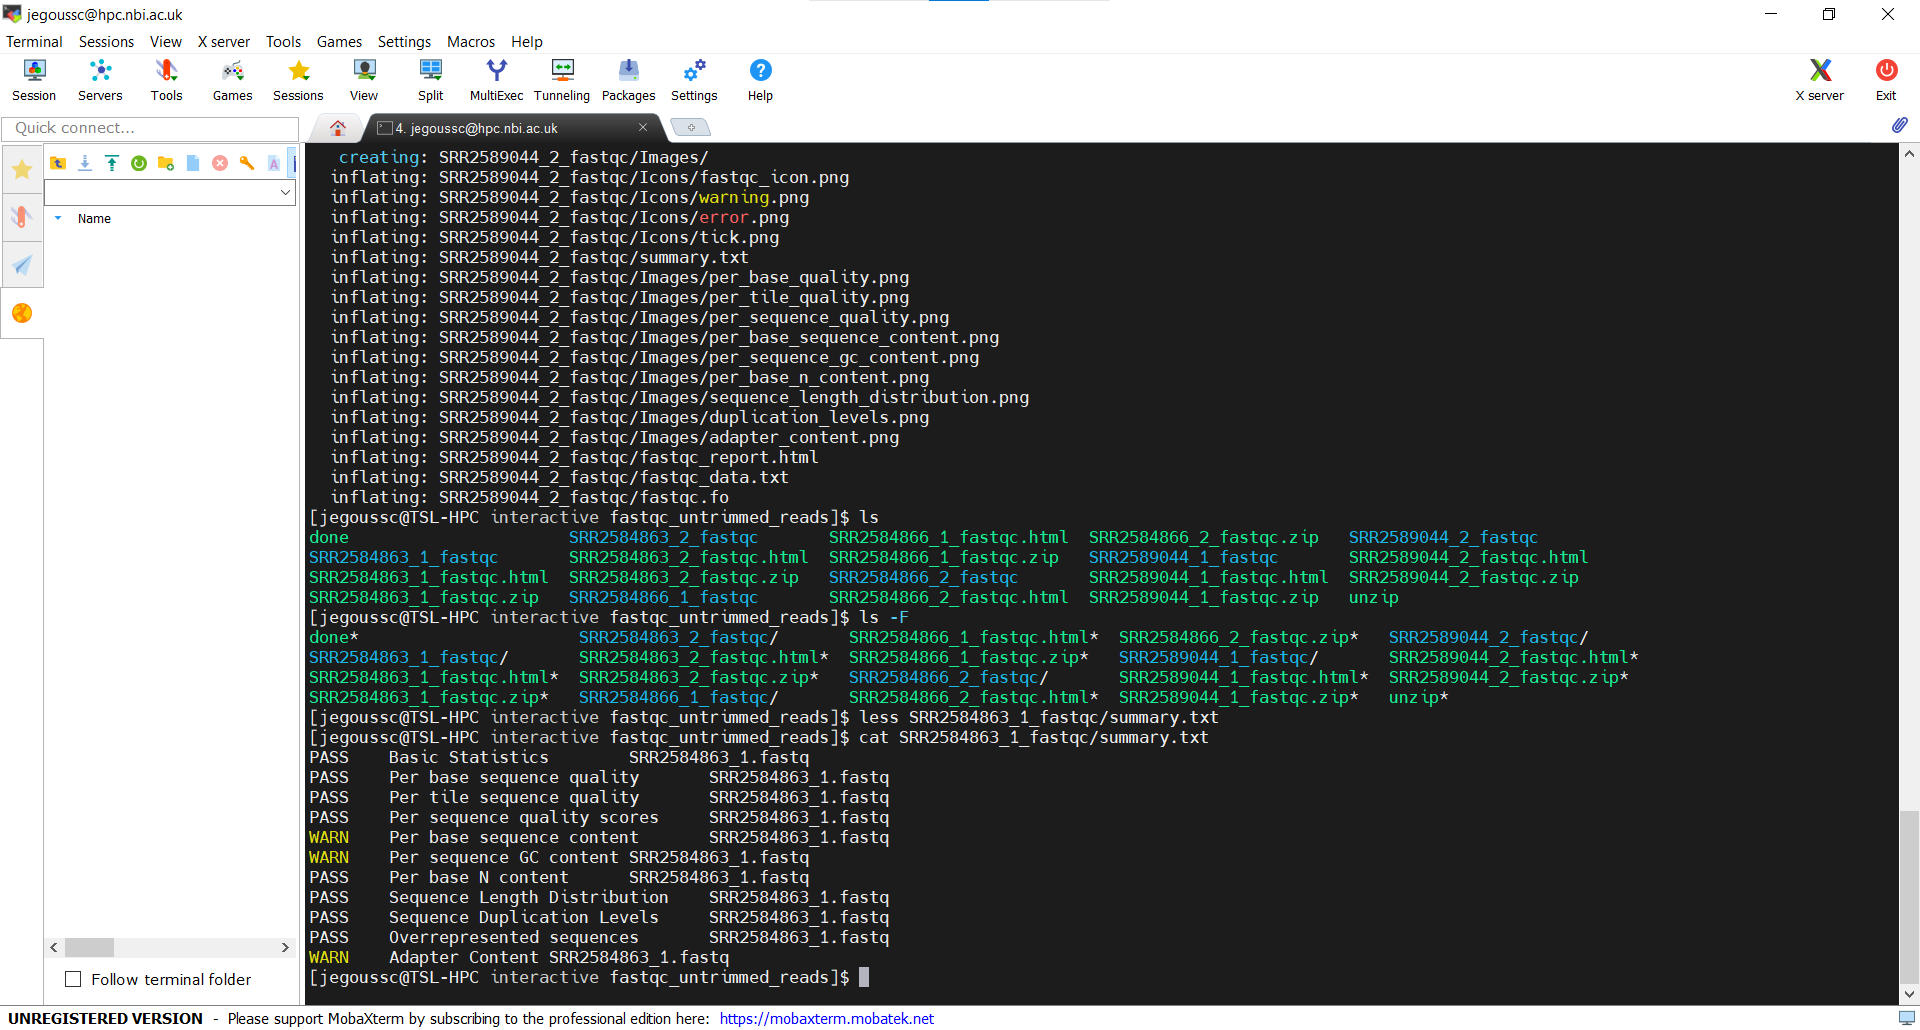
\includegraphics{images/cat-fastqc-summary.png}

\hypertarget{documenting-your-work}{%
\section{Documenting your work}\label{documenting-your-work}}

We can make a record of the results we obtained for all our samples

by concatenating all of our \texttt{summary.txt} files into a single
file using the \texttt{cat} command. We will call this
\texttt{fastqc\_summaries.txt} and move it to
\texttt{\textasciitilde{}/dc\_workshop/docs}.

\begin{Shaded}
\begin{Highlighting}[]
\ExtensionTok{$}\NormalTok{ mkdir }\AttributeTok{{-}p}\NormalTok{ \textasciitilde{}/dc\_workshop/docs/}
\ExtensionTok{$}\NormalTok{ cat }\PreprocessorTok{*}\NormalTok{/summary.txt }\OperatorTok{\textgreater{}}\NormalTok{ \textasciitilde{}/dc\_workshop/docs/fastqc\_summaries.txt}
\end{Highlighting}
\end{Shaded}

\begin{tcolorbox}[enhanced jigsaw, toptitle=1mm, breakable, bottomrule=.15mm, colback=white, toprule=.15mm, opacityback=0, bottomtitle=1mm, coltitle=black, opacitybacktitle=0.6, rightrule=.15mm, colframe=quarto-callout-caution-color-frame, titlerule=0mm, colbacktitle=quarto-callout-caution-color!10!white, title={Exercise}, left=2mm, leftrule=.75mm, arc=.35mm]

Which samples failed at least one of FastQC's quality tests? What
test(s) did those samples fail?

\end{tcolorbox}

\begin{tcolorbox}[enhanced jigsaw, toptitle=1mm, breakable, bottomrule=.15mm, colback=white, toprule=.15mm, opacityback=0, bottomtitle=1mm, coltitle=black, opacitybacktitle=0.6, rightrule=.15mm, colframe=quarto-callout-caution-color-frame, titlerule=0mm, colbacktitle=quarto-callout-caution-color!10!white, title={Solution}, left=2mm, leftrule=.75mm, arc=.35mm]

We can get the list of all failed tests using grep.

\begin{Shaded}
\begin{Highlighting}[]
\ExtensionTok{$}\NormalTok{ cd \textasciitilde{}/dc\_workshop/docs}
\ExtensionTok{$}\NormalTok{ grep FAIL fastqc\_summaries.txt}
\ExtensionTok{FAIL}\NormalTok{    Per base sequence quality       SRR2584863\_2.fastq.gz}
\ExtensionTok{FAIL}\NormalTok{    Per tile sequence quality       SRR2584863\_2.fastq.gz}
\ExtensionTok{FAIL}\NormalTok{    Per base sequence content       SRR2584863\_2.fastq.gz}
\ExtensionTok{FAIL}\NormalTok{    Per base sequence quality       SRR2584866\_1.fastq.gz}
\ExtensionTok{FAIL}\NormalTok{    Per base sequence content       SRR2584866\_1.fastq.gz}
\ExtensionTok{FAIL}\NormalTok{    Adapter Content SRR2584866\_1.fastq.gz}
\ExtensionTok{FAIL}\NormalTok{    Adapter Content SRR2584866\_2.fastq.gz}
\ExtensionTok{FAIL}\NormalTok{    Adapter Content SRR2589044\_1.fastq.gz}
\ExtensionTok{FAIL}\NormalTok{    Per base sequence quality       SRR2589044\_2.fastq.gz}
\ExtensionTok{FAIL}\NormalTok{    Per tile sequence quality       SRR2589044\_2.fastq.gz}
\ExtensionTok{FAIL}\NormalTok{    Per base sequence content       SRR2589044\_2.fastq.gz}
\ExtensionTok{FAIL}\NormalTok{    Adapter Content SRR2589044\_2.fastq.gz}
\end{Highlighting}
\end{Shaded}

\end{tcolorbox}

\hypertarget{summary-1}{%
\section{Summary}\label{summary-1}}

\begin{tcolorbox}[enhanced jigsaw, toptitle=1mm, breakable, bottomrule=.15mm, colback=white, toprule=.15mm, opacityback=0, bottomtitle=1mm, coltitle=black, opacitybacktitle=0.6, rightrule=.15mm, colframe=quarto-callout-note-color-frame, titlerule=0mm, colbacktitle=quarto-callout-note-color!10!white, title=\textcolor{quarto-callout-note-color}{\faInfo}\hspace{0.5em}{Quality encodings vary}, left=2mm, leftrule=.75mm, arc=.35mm]

Although we have used a particular quality encoding system to
demonstrate interpretation of read quality, different sequencing
machines use different encoding systems. This means that, depending on
which sequencer you use to generate your data, a \texttt{\#} may not be
an indicator of a poor quality base call.

This mainly relates to older Solexa/Illumina data, but it is essential
that you know which sequencing platform was used to generate your data,
so that you can tell your quality control program which encoding to use.
If you choose the wrong encoding, you run the risk of throwing away good
reads or (even worse) not throwing away bad reads!

\end{tcolorbox}

\begin{tcolorbox}[enhanced jigsaw, toptitle=1mm, breakable, bottomrule=.15mm, colback=white, toprule=.15mm, opacityback=0, bottomtitle=1mm, coltitle=black, opacitybacktitle=0.6, rightrule=.15mm, colframe=quarto-callout-note-color-frame, titlerule=0mm, colbacktitle=quarto-callout-note-color!10!white, title=\textcolor{quarto-callout-note-color}{\faInfo}\hspace{0.5em}{Same symbols but different meanings}, left=2mm, leftrule=.75mm, arc=.35mm]

Here we see \texttt{\textgreater{}} being used as a shell prompt,
whereas \texttt{\textgreater{}} is also used to redirect output.
Similarly, \texttt{\$} is used as a shell prompt, but, as we saw
earlier, it is also used to ask the shell to get the value of a
variable.

If the \emph{shell} prints \texttt{\textgreater{}} or \texttt{\$} then
it expects you to type something, and the symbol is a prompt.

If \emph{you} type \texttt{\textgreater{}} or \texttt{\$} yourself, it
is an instruction from you that the shell should redirect output or get
the value of a variable.

\end{tcolorbox}

\begin{tcolorbox}[enhanced jigsaw, toptitle=1mm, breakable, bottomrule=.15mm, colback=white, toprule=.15mm, opacityback=0, bottomtitle=1mm, coltitle=black, opacitybacktitle=0.6, rightrule=.15mm, colframe=quarto-callout-important-color-frame, titlerule=0mm, colbacktitle=quarto-callout-important-color!10!white, title=\textcolor{quarto-callout-important-color}{\faExclamation}\hspace{0.5em}{Key points}, left=2mm, leftrule=.75mm, arc=.35mm]

\begin{itemize}
\tightlist
\item
  Quality encodings vary across sequencing platforms.
\item
  \texttt{for} loops let you perform the same set of operations on
  multiple files with a single command.
\end{itemize}

\end{tcolorbox}

\bookmarksetup{startatroot}

\hypertarget{trimming-and-filtering}{%
\chapter{Trimming and filtering}\label{trimming-and-filtering}}

\begin{tcolorbox}[enhanced jigsaw, toptitle=1mm, breakable, bottomrule=.15mm, colback=white, toprule=.15mm, opacityback=0, bottomtitle=1mm, coltitle=black, opacitybacktitle=0.6, rightrule=.15mm, colframe=quarto-callout-note-color-frame, titlerule=0mm, colbacktitle=quarto-callout-note-color!10!white, title={⏳ Time}, left=2mm, leftrule=.75mm, arc=.35mm]

\begin{itemize}
\tightlist
\item
  Teaching: 30 min
\item
  Exercises: 25 min
\end{itemize}

\end{tcolorbox}

\begin{tcolorbox}[enhanced jigsaw, toptitle=1mm, breakable, bottomrule=.15mm, colback=white, toprule=.15mm, opacityback=0, bottomtitle=1mm, coltitle=black, opacitybacktitle=0.6, rightrule=.15mm, colframe=quarto-callout-tip-color-frame, titlerule=0mm, colbacktitle=quarto-callout-tip-color!10!white, title={🤔 Question}, left=2mm, leftrule=.75mm, arc=.35mm]

\begin{itemize}
\tightlist
\item
  How can I get rid of sequence data that does not meet my quality
  standards?
\end{itemize}

\end{tcolorbox}

\begin{tcolorbox}[enhanced jigsaw, toptitle=1mm, breakable, bottomrule=.15mm, colback=white, toprule=.15mm, opacityback=0, bottomtitle=1mm, coltitle=black, opacitybacktitle=0.6, rightrule=.15mm, colframe=quarto-callout-important-color-frame, titlerule=0mm, colbacktitle=quarto-callout-important-color!10!white, title={🎯 Objectives}, left=2mm, leftrule=.75mm, arc=.35mm]

\begin{itemize}
\tightlist
\item
  Clean FASTQ reads using Trimmomatic.
\item
  Select and set multiple options for command-line bioinformatic tools.
\item
  Write for loops with two variables.
\end{itemize}

\end{tcolorbox}

\hypertarget{cleaning-reads}{%
\section{Cleaning reads}\label{cleaning-reads}}

In the previous episode, we took a high-level look at the quality of
each of our samples using FastQC. We visualized per-base quality graphs
showing the distribution of read quality at each base across all reads
in a sample and extracted information about which samples fail which
quality checks. Some of our samples failed quite a few quality metrics
used by FastQC. This does not mean, though, that our samples should be
thrown out! It is very common to have some quality metrics fail, and
this may or may not be a problem for your downstream application. For
our variant calling workflow, we will be removing some of the low
quality sequences to reduce our false positive rate due to sequencing
error.

We will use a program called Trimmomatic (Bolger, Lohse, and Usadel
2014) to filter poor quality reads and trim poor quality bases from our
samples.

\begin{tcolorbox}[enhanced jigsaw, toptitle=1mm, breakable, bottomrule=.15mm, colback=white, toprule=.15mm, opacityback=0, bottomtitle=1mm, coltitle=black, opacitybacktitle=0.6, rightrule=.15mm, colframe=quarto-callout-important-color-frame, titlerule=0mm, colbacktitle=quarto-callout-important-color!10!white, title=\textcolor{quarto-callout-important-color}{\faExclamation}\hspace{0.5em}{Important}, left=2mm, leftrule=.75mm, arc=.35mm]

Make sure to be connected to the server.

\end{tcolorbox}

Let's load Trimmomatic to our interactive session on the server.

\begin{Shaded}
\begin{Highlighting}[]
\ExtensionTok{$}\NormalTok{ source package /nbi/software/production/bin/trimmomatic{-}0.39}
\ExtensionTok{loaded}\NormalTok{ /nbi/software/production/bin/trimmomatic{-}0.39}
\end{Highlighting}
\end{Shaded}

\hypertarget{trimmomatic-options}{%
\subsection{Trimmomatic options}\label{trimmomatic-options}}

Trimmomatic has a variety of options to trim your reads. If we run the
following command, we can see some of our options.

\begin{Shaded}
\begin{Highlighting}[]
\ExtensionTok{$}\NormalTok{ trimmomatic}
\end{Highlighting}
\end{Shaded}

Which will give you the following output:

\begin{verbatim}
Usage: 
       PE [-version] [-threads <threads>] [-phred33|-phred64] [-trimlog <trimLogFile>] [-summary <statsSummaryFile>] [-quiet] [-validatePairs] [-basein <inputBase> | <inputFile1> <inputFile2>] [-baseout <outputBase> | <outputFile1P> <outputFile1U> <outputFile2P> <outputFile2U>] <trimmer1>...
   or: 
       SE [-version] [-threads <threads>] [-phred33|-phred64] [-trimlog <trimLogFile>] [-summary <statsSummaryFile>] [-quiet] <inputFile> <outputFile> <trimmer1>...
   or: 
       -version
\end{verbatim}

This output shows us that we must first specify whether we have paired
end (\texttt{PE}) or single end (\texttt{SE}) reads. Next, we specify
what flag we would like to run. For example, you can specify
\texttt{threads} to indicate the number of processors on your computer
that you want Trimmomatic to use. In most cases using multiple threads
(processors) can help to run the trimming faster. These flags are not
necessary, but they can give you more control over the command. The
flags are followed by positional arguments, meaning the order in which
you specify them is important. In paired end mode, Trimmomatic expects
the two input files, and then the names of the output files. These files
are described below. While, in single end mode, Trimmomatic will expect
1 file as input, after which you can enter the optional settings and
lastly the name of the output file.

\begin{longtable}[]{@{}
  >{\raggedright\arraybackslash}p{(\columnwidth - 2\tabcolsep) * \real{0.1593}}
  >{\raggedright\arraybackslash}p{(\columnwidth - 2\tabcolsep) * \real{0.8407}}@{}}
\toprule\noalign{}
\begin{minipage}[b]{\linewidth}\raggedright
option
\end{minipage} & \begin{minipage}[b]{\linewidth}\raggedright
meaning
\end{minipage} \\
\midrule\noalign{}
\endhead
\bottomrule\noalign{}
\endlastfoot
\textless inputFile1\textgreater{} & Input reads to be trimmed.
Typically the file name will contain an \texttt{\_1} or \texttt{\_R1} in
the name. \\
\textless inputFile2\textgreater{} & Input reads to be trimmed.
Typically the file name will contain an \texttt{\_2} or \texttt{\_R2} in
the name. \\
\textless outputFile1P\textgreater{} & Output file that contains
surviving pairs from the \texttt{\_1} file. \\
\textless outputFile1U\textgreater{} & Output file that contains
orphaned reads from the \texttt{\_1} file. \\
\textless outputFile2P\textgreater{} & Output file that contains
surviving pairs from the \texttt{\_2} file. \\
\textless outputFile2U\textgreater{} & Output file that contains
orphaned reads from the \texttt{\_2} file. \\
\end{longtable}

The last thing Trimmomatic expects to see is the trimming parameters:

\begin{longtable}[]{@{}
  >{\raggedright\arraybackslash}p{(\columnwidth - 2\tabcolsep) * \real{0.1339}}
  >{\raggedright\arraybackslash}p{(\columnwidth - 2\tabcolsep) * \real{0.8661}}@{}}
\toprule\noalign{}
\begin{minipage}[b]{\linewidth}\raggedright
step
\end{minipage} & \begin{minipage}[b]{\linewidth}\raggedright
meaning
\end{minipage} \\
\midrule\noalign{}
\endhead
\bottomrule\noalign{}
\endlastfoot
\texttt{ILLUMINACLIP} & Perform adapter removal. \\
\texttt{SLIDINGWINDOW} & Perform sliding window trimming, cutting once
the average quality within the window falls below a threshold. \\
\texttt{LEADING} & Cut bases off the start of a read, if below a
threshold quality. \\
\texttt{TRAILING} & Cut bases off the end of a read, if below a
threshold quality. \\
\texttt{CROP} & Cut the read to a specified length. \\
\texttt{HEADCROP} & Cut the specified number of bases from the start of
the read. \\
\texttt{MINLEN} & Drop an entire read if it is below a specified
length. \\
\texttt{TOPHRED33} & Convert quality scores to Phred-33. \\
\texttt{TOPHRED64} & Convert quality scores to Phred-64. \\
\end{longtable}

We will use only a few of these options and trimming steps in our
analysis. It is important to understand the steps you are using to clean
your data. For more information about the Trimmomatic arguments and
options, see
\href{http://www.usadellab.org/cms/uploads/supplementary/Trimmomatic/TrimmomaticManual_V0.32.pdf}{the
Trimmomatic manual}.

\hypertarget{running-trimmomatic}{%
\subsection{Running Trimmomatic}\label{running-trimmomatic}}

Now we will run Trimmomatic on our data. To begin, navigate to your
\texttt{untrimmed\_fastq} data directory:

\begin{Shaded}
\begin{Highlighting}[]
\ExtensionTok{$}\NormalTok{ cd \textasciitilde{}/dc\_workshop/data/untrimmed\_fastq}
\end{Highlighting}
\end{Shaded}

We are going to run Trimmomatic on one of our paired-end samples. While
using FastQC we saw that Nextera adapters were present in our samples.
The adapter sequences came with the installation of Trimmomatic.

We will also use a sliding window of size 4 that will remove bases if
their phred score is below 20 (like in our example above). We will also
discard any reads that do not have at least 25 bases remaining after
this trimming step. Three additional pieces of code are also added to
the end of the ILLUMINACLIP step. These three additional numbers
(2:40:15) tell Trimmomatic how to handle sequence matches to the Nextera
adapters. A detailed explanation of how they work is advanced for this
particular lesson. For now we will use these numbers as a default and
recognize they are needed to for Trimmomatic to run properly.

\begin{Shaded}
\begin{Highlighting}[]
\ExtensionTok{$}\NormalTok{ trimmomatic PE SRR2589044\_1.fastq.gz SRR2589044\_2.fastq.gz }\DataTypeTok{\textbackslash{}}
\NormalTok{                SRR2589044\_1.trim.fastq.gz SRR2589044\_1un.trim.fastq.gz }\DataTypeTok{\textbackslash{}}
\NormalTok{                SRR2589044\_2.trim.fastq.gz SRR2589044\_2un.trim.fastq.gz }\DataTypeTok{\textbackslash{}}
\NormalTok{                SLIDINGWINDOW:4:20 }\DataTypeTok{\textbackslash{}}
\NormalTok{                MINLEN:25 }\DataTypeTok{\textbackslash{}}
\NormalTok{                ILLUMINACLIP:NexteraPE{-}PE.fa:2:40:15}
\end{Highlighting}
\end{Shaded}

This command will take about two minutes to run.

\begin{tcolorbox}[enhanced jigsaw, toptitle=1mm, breakable, bottomrule=.15mm, colback=white, toprule=.15mm, opacityback=0, bottomtitle=1mm, coltitle=black, opacitybacktitle=0.6, rightrule=.15mm, colframe=quarto-callout-note-color-frame, titlerule=0mm, colbacktitle=quarto-callout-note-color!10!white, title=\textcolor{quarto-callout-note-color}{\faInfo}\hspace{0.5em}{About multiline commands}, left=2mm, leftrule=.75mm, arc=.35mm]

Some of the commands we ran in this lesson are long! When typing a long
command into your terminal, you can use the \texttt{\textbackslash{}}
character to separate code chunks onto separate lines. This can make
your code more readable.

\end{tcolorbox}

\begin{longtable}[]{@{}
  >{\raggedright\arraybackslash}p{(\columnwidth - 2\tabcolsep) * \real{0.2302}}
  >{\raggedright\arraybackslash}p{(\columnwidth - 2\tabcolsep) * \real{0.7698}}@{}}
\toprule\noalign{}
\begin{minipage}[b]{\linewidth}\raggedright
code
\end{minipage} & \begin{minipage}[b]{\linewidth}\raggedright
meaning
\end{minipage} \\
\midrule\noalign{}
\endhead
\bottomrule\noalign{}
\endlastfoot
\texttt{PE} & that it will be taking a paired end file as input \\
\texttt{-threads\ 4} & to use four computing threads to run (this will
speed up our run) \\
\texttt{SRR2589044\_1.fastq} & the first input file name \\
\texttt{SRR2589044\_2.fastq} & the second input file name \\
\texttt{SRR2589044\_1.trimmed.fastq} & the output file for surviving
pairs from the \texttt{\_1} file \\
\texttt{SRR2589044\_1un.trimmed.fastq} & the output file for orphaned
reads from the \texttt{\_1} file \\
\texttt{SRR2589044\_2.trimmed.fastq} & the output file for surviving
pairs from the \texttt{\_2} file \\
\texttt{SRR2589044\_2un.trimmed.fastq} & the output file for orphaned
reads from the \texttt{\_2} file \\
\texttt{ILLUMINACLIP:SRR\_adapters.fa} & to clip the Illumina adapters
from the input file using the adapter sequences listed in
\texttt{SRR\_adapters.fa} \\
\texttt{SLIDINGWINDOW:4:20} & to use a sliding window of size 4 that
will remove bases if their phred score is below 20 \\
\texttt{MINLEN:25} & minimum length of 25 nucleotides. \\
\end{longtable}

The output should look like this:

\begin{verbatim}
TrimmomaticPE: Started with arguments:
 SRR2589044_1.fastq.gz SRR2589044_2.fastq.gz SRR2589044_1.trim.fastq.gz SRR2589044_1un.trim.fastq.gz SRR2589044_2.trim.fastq.gz SRR2589044_2un.trim.fastq.gz SLIDINGWINDOW:4:20 MINLEN:25 ILLUMINACLIP:NexteraPE-PE.fa:2:40:15
Multiple cores found: Using 2 threads
Using PrefixPair: 'AGATGTGTATAAGAGACAG' and 'AGATGTGTATAAGAGACAG'
Using Long Clipping Sequence: 'GTCTCGTGGGCTCGGAGATGTGTATAAGAGACAG'
Using Long Clipping Sequence: 'TCGTCGGCAGCGTCAGATGTGTATAAGAGACAG'
Using Long Clipping Sequence: 'CTGTCTCTTATACACATCTCCGAGCCCACGAGAC'
Using Long Clipping Sequence: 'CTGTCTCTTATACACATCTGACGCTGCCGACGA'
ILLUMINACLIP: Using 1 prefix pairs, 4 forward/reverse sequences, 0 forward only sequences, 0 reverse only sequences
Quality encoding detected as phred33
Input Read Pairs: 1107090 Both Surviving: 885220 (79.96%) Forward Only Surviving: 216472 (19.55%) Reverse Only Surviving: 2850 (0.26%) Dropped: 2548 (0.23%)
TrimmomaticPE: Completed successfully
\end{verbatim}

\begin{tcolorbox}[enhanced jigsaw, toptitle=1mm, breakable, bottomrule=.15mm, colback=white, toprule=.15mm, opacityback=0, bottomtitle=1mm, coltitle=black, opacitybacktitle=0.6, rightrule=.15mm, colframe=quarto-callout-caution-color-frame, titlerule=0mm, colbacktitle=quarto-callout-caution-color!10!white, title={Exercise}, left=2mm, leftrule=.75mm, arc=.35mm]

Use the output from your Trimmomatic command to answer the following
questions.

\begin{enumerate}
\def\labelenumi{\arabic{enumi})}
\tightlist
\item
  What percent of reads did we discard from our sample?
\item
  What percent of reads did we keep both pairs?
\end{enumerate}

\end{tcolorbox}

\begin{tcolorbox}[enhanced jigsaw, toptitle=1mm, breakable, bottomrule=.15mm, colback=white, toprule=.15mm, opacityback=0, bottomtitle=1mm, coltitle=black, opacitybacktitle=0.6, rightrule=.15mm, colframe=quarto-callout-caution-color-frame, titlerule=0mm, colbacktitle=quarto-callout-caution-color!10!white, title={Solution}, left=2mm, leftrule=.75mm, arc=.35mm]

\begin{enumerate}
\def\labelenumi{\arabic{enumi})}
\tightlist
\item
  0.23\%
\item
  79.96\%
\end{enumerate}

\end{tcolorbox}

You may have noticed that Trimmomatic automatically detected the quality
encoding of our sample. It is always a good idea to double-check this or
to enter the quality encoding manually.

We can confirm that we have our output files:

\begin{Shaded}
\begin{Highlighting}[]
\ExtensionTok{$}\NormalTok{ ls SRR2589044}\PreprocessorTok{*}
\ExtensionTok{SRR2589044\_1.fastq.gz}\NormalTok{       SRR2589044\_1un.trim.fastq.gz  SRR2589044\_2.trim.fastq.gz}
\ExtensionTok{SRR2589044\_1.trim.fastq.gz}\NormalTok{  SRR2589044\_2.fastq.gz         SRR2589044\_2un.trim.fastq.gz}
\end{Highlighting}
\end{Shaded}

The output files are also FASTQ files. It should be smaller than our
input file, because we have removed reads. We can confirm this:

\begin{Shaded}
\begin{Highlighting}[]
\ExtensionTok{$}\NormalTok{ ls SRR2589044}\PreprocessorTok{*} \AttributeTok{{-}l} \AttributeTok{{-}h}
\ExtensionTok{{-}rwx{-}{-}{-}{-}{-}{-}}\NormalTok{ 1 }\PreprocessorTok{[}\SpecialStringTok{username}\PreprocessorTok{]}\NormalTok{ TSL\_20 124M Aug 11 11:00 SRR2589044\_1.fastq.gz}
\ExtensionTok{{-}rwx{-}{-}{-}{-}{-}{-}}\NormalTok{ 1 }\PreprocessorTok{[}\SpecialStringTok{username}\PreprocessorTok{]}\NormalTok{ TSL\_20 105M Aug 11 15:56 SRR2589044\_1.trim.fastq.gz}
\ExtensionTok{{-}rwx{-}{-}{-}{-}{-}{-}}\NormalTok{ 1 }\PreprocessorTok{[}\SpecialStringTok{username}\PreprocessorTok{]}\NormalTok{ TSL\_20 8.4M Aug 11 15:56 SRR2589044\_1un.trim.fastq.gz}
\ExtensionTok{{-}rwx{-}{-}{-}{-}{-}{-}}\NormalTok{ 1 }\PreprocessorTok{[}\SpecialStringTok{username}\PreprocessorTok{]}\NormalTok{ TSL\_20 128M Aug 11 11:01 SRR2589044\_2.fastq.gz}
\ExtensionTok{{-}rwx{-}{-}{-}{-}{-}{-}}\NormalTok{ 1 }\PreprocessorTok{[}\SpecialStringTok{username}\PreprocessorTok{]}\NormalTok{ TSL\_20 103M Aug 11 15:56 SRR2589044\_2.trim.fastq.gz}
\ExtensionTok{{-}rwx{-}{-}{-}{-}{-}{-}}\NormalTok{ 1 }\PreprocessorTok{[}\SpecialStringTok{username}\PreprocessorTok{]}\NormalTok{ TSL\_20 276K Aug 11 15:56 SRR2589044\_2un.trim.fastq.gz}
\end{Highlighting}
\end{Shaded}

We have just successfully run Trimmomatic on one of our FASTQ files!
However, there is some bad news. Trimmomatic can only operate on one
sample at a time and we have more than one sample. The good news is that
we can use a \texttt{for} loop to iterate through our sample files
quickly!

We unzipped one of our files before to work with it, let's compress it
again before we run our for loop.

\begin{Shaded}
\begin{Highlighting}[]
\ExtensionTok{$}\NormalTok{ gzip SRR2584863\_1.fastq }
\end{Highlighting}
\end{Shaded}

\begin{tcolorbox}[enhanced jigsaw, toptitle=1mm, breakable, bottomrule=.15mm, colback=white, toprule=.15mm, opacityback=0, bottomtitle=1mm, coltitle=black, opacitybacktitle=0.6, rightrule=.15mm, colframe=quarto-callout-warning-color-frame, titlerule=0mm, colbacktitle=quarto-callout-warning-color!10!white, title=\textcolor{quarto-callout-warning-color}{\faExclamationTriangle}\hspace{0.5em}{Warning}, left=2mm, leftrule=.75mm, arc=.35mm]

Do not copy-paste the four lines at once. You must type the \texttt{for}
loop line by line!

\end{tcolorbox}

\begin{Shaded}
\begin{Highlighting}[]
\ExtensionTok{$}\NormalTok{ for infile in }\PreprocessorTok{*}\NormalTok{\_1.fastq.gz}
\OperatorTok{\textgreater{}}\NormalTok{ do}
\OperatorTok{\textgreater{}}\NormalTok{   base=}\VariableTok{$(}\FunctionTok{basename} \VariableTok{$\{infile\}}\NormalTok{ \_1.fastq.gz}\VariableTok{)}
\OperatorTok{\textgreater{}}\NormalTok{   trimmomatic }\ExtensionTok{PE} \VariableTok{$\{infile\}} \VariableTok{$\{base\}}\NormalTok{\_2.fastq.gz }\DataTypeTok{\textbackslash{}}
\OperatorTok{\textgreater{}}                \VariableTok{$\{base\}}\NormalTok{\_1.trim.fastq.gz }\VariableTok{$\{base\}}\NormalTok{\_1un.trim.fastq.gz }\DataTypeTok{\textbackslash{}}
\OperatorTok{\textgreater{}}                \VariableTok{$\{base\}}\NormalTok{\_2.trim.fastq.gz }\VariableTok{$\{base\}}\NormalTok{\_2un.trim.fastq.gz }\DataTypeTok{\textbackslash{}}
\OperatorTok{\textgreater{}}\NormalTok{                SLIDINGWINDOW:4:20 }\DataTypeTok{\textbackslash{}}
\OperatorTok{\textgreater{}}\NormalTok{                MINLEN:25 }\DataTypeTok{\textbackslash{}}
\OperatorTok{\textgreater{}}\NormalTok{                ILLUMINACLIP:NexteraPE{-}PE.fa:2:40:15 }
\OperatorTok{\textgreater{}}\NormalTok{ done}
\end{Highlighting}
\end{Shaded}

Go ahead and run the for loop. It should take about 12 minutes for
Trimmomatic to run for each of our six input files.

Once it is done running, take a look at your directory contents.

\begin{Shaded}
\begin{Highlighting}[]
\ExtensionTok{$}\NormalTok{ ls}
\ExtensionTok{SRR2584863\_1.fastq.gz}\NormalTok{         SRR2584866\_2.fastq.gz}
\ExtensionTok{SRR2584863\_1.trim.fastq.gz}\NormalTok{    SRR2584866\_2.trim.fastq.gz}
\ExtensionTok{SRR2584863\_1un.trim.fastq.gz}\NormalTok{  SRR2584866\_2un.trim.fastq.gz}
\ExtensionTok{SRR2584863\_2.fastq.gz}\NormalTok{         SRR2589044\_1.fastq.gz}
\ExtensionTok{SRR2584863\_2.trim.fastq.gz}\NormalTok{    SRR2589044\_1.trim.fastq.gz}
\ExtensionTok{SRR2584863\_2un.trim.fastq.gz}\NormalTok{  SRR2589044\_1un.trim.fastq.gz}
\ExtensionTok{SRR2584866\_1.fastq.gz}\NormalTok{         SRR2589044\_2.fastq.gz}
\ExtensionTok{SRR2584866\_1.trim.fastq.gz}\NormalTok{    SRR2589044\_2.trim.fastq.gz}
\ExtensionTok{SRR2584866\_1un.trim.fastq.gz}\NormalTok{  SRR2589044\_2un.trim.fastq.gz}
\end{Highlighting}
\end{Shaded}

\begin{tcolorbox}[enhanced jigsaw, toptitle=1mm, breakable, bottomrule=.15mm, colback=white, toprule=.15mm, opacityback=0, bottomtitle=1mm, coltitle=black, opacitybacktitle=0.6, rightrule=.15mm, colframe=quarto-callout-note-color-frame, titlerule=0mm, colbacktitle=quarto-callout-note-color!10!white, title=\textcolor{quarto-callout-note-color}{\faInfo}\hspace{0.5em}{Note}, left=2mm, leftrule=.75mm, arc=.35mm]

You will notice that even though we ran Trimmomatic on file
\texttt{SRR2589044} before running the for loop, there is only one set
of files for it. Because we matched the ending \texttt{\_1.fastq.gz}, we
re-ran Trimmomatic on this file, overwriting our first results. That is
ok, but it is good to be aware that it happened.

\end{tcolorbox}

We have now completed the trimming and filtering steps of our quality
control process! Before we move on, let's move our trimmed FASTQ files
to a new subdirectory within our \texttt{data/} directory.

\begin{Shaded}
\begin{Highlighting}[]
\ExtensionTok{$}\NormalTok{ cd \textasciitilde{}/dc\_workshop/data/untrimmed\_fastq}
\ExtensionTok{$}\NormalTok{ mkdir ../trimmed\_fastq}
\ExtensionTok{$}\NormalTok{ mv }\PreprocessorTok{*}\NormalTok{.trim}\PreprocessorTok{*}\NormalTok{ ../trimmed\_fastq}
\ExtensionTok{$}\NormalTok{ cd ../trimmed\_fastq}
\ExtensionTok{$}\NormalTok{ ls}
\ExtensionTok{SRR2584863\_1.trim.fastq.gz}\NormalTok{    SRR2584866\_1.trim.fastq.gz    SRR2589044\_1.trim.fastq.gz}
\ExtensionTok{SRR2584863\_1un.trim.fastq.gz}\NormalTok{  SRR2584866\_1un.trim.fastq.gz  SRR2589044\_1un.trim.fastq.gz}
\ExtensionTok{SRR2584863\_2.trim.fastq.gz}\NormalTok{    SRR2584866\_2.trim.fastq.gz    SRR2589044\_2.trim.fastq.gz}
\ExtensionTok{SRR2584863\_2un.trim.fastq.gz}\NormalTok{  SRR2584866\_2un.trim.fastq.gz  SRR2589044\_2un.trim.fastq.gz}
\end{Highlighting}
\end{Shaded}

\begin{tcolorbox}[enhanced jigsaw, toptitle=1mm, breakable, bottomrule=.15mm, colback=white, toprule=.15mm, opacityback=0, bottomtitle=1mm, coltitle=black, opacitybacktitle=0.6, rightrule=.15mm, colframe=quarto-callout-caution-color-frame, titlerule=0mm, colbacktitle=quarto-callout-caution-color!10!white, title={Bonus exercise}, left=2mm, leftrule=.75mm, arc=.35mm]

Now that our samples have gone through quality control, they should
perform better on the quality tests run by FastQC. Go ahead and re-run
FastQC on your trimmed FASTQ files and visualize the HTML files to see
whether your per base sequence quality is higher after trimming.

\end{tcolorbox}

\begin{tcolorbox}[enhanced jigsaw, toptitle=1mm, breakable, bottomrule=.15mm, colback=white, toprule=.15mm, opacityback=0, bottomtitle=1mm, coltitle=black, opacitybacktitle=0.6, rightrule=.15mm, colframe=quarto-callout-caution-color-frame, titlerule=0mm, colbacktitle=quarto-callout-caution-color!10!white, title={Solution}, left=2mm, leftrule=.75mm, arc=.35mm]

\begin{Shaded}
\begin{Highlighting}[]
\ExtensionTok{$}\NormalTok{ fastqc \textasciitilde{}/dc\_workshop/data/trimmed\_fastq/}\PreprocessorTok{*}\NormalTok{.fastq}\PreprocessorTok{*}
\end{Highlighting}
\end{Shaded}

Then output files can be transferred to the local computer to be
visualized.

After trimming and filtering, our overall quality is much higher, we
have a distribution of sequence lengths, and more samples pass adapter
content. However, quality trimming is not perfect, and some programs are
better at removing some sequences than others. Because our sequences
still contain 3' adapters, it could be important to explore other
trimming tools like
\href{http://cutadapt.readthedocs.io/en/stable/}{Cutadapt} (Martin 2011)
to remove these, depending on your downstream application. Trimmomatic
did pretty well though, and its performance is good enough for our
workflow.

\end{tcolorbox}

\hypertarget{summary-2}{%
\section{Summary}\label{summary-2}}

\begin{tcolorbox}[enhanced jigsaw, toptitle=1mm, breakable, bottomrule=.15mm, colback=white, toprule=.15mm, opacityback=0, bottomtitle=1mm, coltitle=black, opacitybacktitle=0.6, rightrule=.15mm, colframe=quarto-callout-important-color-frame, titlerule=0mm, colbacktitle=quarto-callout-important-color!10!white, title=\textcolor{quarto-callout-important-color}{\faExclamation}\hspace{0.5em}{Key points}, left=2mm, leftrule=.75mm, arc=.35mm]

\begin{itemize}
\tightlist
\item
  The options you set for the command-line tools you use are important!
\item
  Data cleaning is an essential step in a genomics workflow.
\end{itemize}

\end{tcolorbox}

\bookmarksetup{startatroot}

\hypertarget{sec-variant-calling-workflow}{%
\chapter{Variant calling workflow}\label{sec-variant-calling-workflow}}

\begin{tcolorbox}[enhanced jigsaw, toptitle=1mm, breakable, bottomrule=.15mm, colback=white, toprule=.15mm, opacityback=0, bottomtitle=1mm, coltitle=black, opacitybacktitle=0.6, rightrule=.15mm, colframe=quarto-callout-note-color-frame, titlerule=0mm, colbacktitle=quarto-callout-note-color!10!white, title={⏳ Time}, left=2mm, leftrule=.75mm, arc=.35mm]

\begin{itemize}
\tightlist
\item
  Teaching: 35 min
\item
  Exercises: 25 min
\end{itemize}

\end{tcolorbox}

\begin{tcolorbox}[enhanced jigsaw, toptitle=1mm, breakable, bottomrule=.15mm, colback=white, toprule=.15mm, opacityback=0, bottomtitle=1mm, coltitle=black, opacitybacktitle=0.6, rightrule=.15mm, colframe=quarto-callout-tip-color-frame, titlerule=0mm, colbacktitle=quarto-callout-tip-color!10!white, title={🤔 Question}, left=2mm, leftrule=.75mm, arc=.35mm]

\begin{itemize}
\tightlist
\item
  How do I find sequence variants between my sample and a reference
  genome?
\end{itemize}

\end{tcolorbox}

\begin{tcolorbox}[enhanced jigsaw, toptitle=1mm, breakable, bottomrule=.15mm, colback=white, toprule=.15mm, opacityback=0, bottomtitle=1mm, coltitle=black, opacitybacktitle=0.6, rightrule=.15mm, colframe=quarto-callout-important-color-frame, titlerule=0mm, colbacktitle=quarto-callout-important-color!10!white, title={🎯 Objectives}, left=2mm, leftrule=.75mm, arc=.35mm]

\begin{itemize}
\tightlist
\item
  Understand the steps involved in variant calling.
\item
  Describe the types of data formats encountered during variant calling.
\item
  Use command line tools to perform variant calling.
\end{itemize}

\end{tcolorbox}

We mentioned before that we are working with files from a long-term
evolution study of an \emph{E. coli} population (designated Ara-3). Now
that we have looked at our data to make sure that it is high quality,
and removed low-quality base calls, we can perform variant calling to
see how the population changed over time. We care how this population
changed relative to the original population, \emph{E. coli} strain
REL606. Therefore, we will align each of our samples to the \emph{E.
coli} REL606 reference genome, and see what differences exist in our
reads versus the genome.

\hypertarget{alignment-to-a-reference-genome}{%
\section{Alignment to a reference
genome}\label{alignment-to-a-reference-genome}}

We perform read alignment or mapping to determine where in the genome
our reads originated from. There are a number of tools to choose from
and, while there is no gold standard, there are some tools that are
better suited for particular NGS analyses. We will be using the Burrows
Wheeler Aligner (BWA) by Li and Durbin (2010), which is a software
package for mapping low-divergent sequences against a large reference
genome.

The alignment process consists of two steps:

\begin{enumerate}
\def\labelenumi{\arabic{enumi}.}
\tightlist
\item
  Indexing the reference genome
\item
  Aligning the reads to the reference genome
\end{enumerate}

\hypertarget{setting-up}{%
\section{Setting up}\label{setting-up}}

\hypertarget{option-1-copy-from-shared-directory-on-the-hpc}{%
\subsection{Option 1: Copy from shared directory on the
HPC}\label{option-1-copy-from-shared-directory-on-the-hpc}}

You should already have all the files from the previous section where we
copied all files we need including the reference genome and small
dataset to your directory. Now:

Unzip the reference genome

\begin{Shaded}
\begin{Highlighting}[]
\ExtensionTok{$}\NormalTok{ gunzip ecoli\_rel606.fasta.gz}
\end{Highlighting}
\end{Shaded}

\begin{tcolorbox}[enhanced jigsaw, toptitle=1mm, breakable, bottomrule=.15mm, colback=white, toprule=.15mm, opacityback=0, bottomtitle=1mm, coltitle=black, opacitybacktitle=0.6, rightrule=.15mm, colframe=quarto-callout-caution-color-frame, titlerule=0mm, colbacktitle=quarto-callout-caution-color!10!white, title={Exercise}, left=2mm, leftrule=.75mm, arc=.35mm]

We saved this file as \texttt{data/ref\_genome/ecoli\_rel606.fasta.gz}
and then decompressed it. What is the real name of the genome?

\end{tcolorbox}

\begin{tcolorbox}[enhanced jigsaw, toptitle=1mm, breakable, bottomrule=.15mm, colback=white, toprule=.15mm, opacityback=0, bottomtitle=1mm, coltitle=black, opacitybacktitle=0.6, rightrule=.15mm, colframe=quarto-callout-caution-color-frame, titlerule=0mm, colbacktitle=quarto-callout-caution-color!10!white, title={Solution}, left=2mm, leftrule=.75mm, arc=.35mm]

\begin{Shaded}
\begin{Highlighting}[]
\ExtensionTok{$}\NormalTok{ head data/ref\_genome/ecoli\_rel606.fasta}
\end{Highlighting}
\end{Shaded}

The name of the sequence follows the \texttt{\textgreater{}} character.
The name is
\texttt{CP000819.1\ Escherichia\ coli\ B\ str.\ REL606,\ complete\ genome}.
Keep this chromosome name (\texttt{CP000819.1}) in mind, as we will use
it later in the lesson.

\end{tcolorbox}

We will also have a set of trimmed FASTQ files to work with. These are
small subsets of our real trimmed data, and will enable us to run our
variant calling workflow quite quickly.

\begin{Shaded}
\begin{Highlighting}[]
\ExtensionTok{$}\NormalTok{ ls \textasciitilde{}/dc\_workshop/data/trimmed\_fastq\_small}
\end{Highlighting}
\end{Shaded}

\hypertarget{index-the-reference-genome}{%
\section{Index the reference genome}\label{index-the-reference-genome}}

Let's make sure we are back in the \texttt{dc\_workshop} directory and
that the two directories are where we hope they are:

\begin{Shaded}
\begin{Highlighting}[]
\ExtensionTok{$}\NormalTok{ cd \textasciitilde{}/dc\_workshop/}
\ExtensionTok{$}\NormalTok{ ls }\AttributeTok{{-}F}\NormalTok{ data/}
\ExtensionTok{ref\_genome/}\NormalTok{  trimmed\_fastq\_small/  untrimmed\_fastq/}
\ExtensionTok{$}\NormalTok{ ls }\AttributeTok{{-}F}\NormalTok{ data/ref\_genome/}
\ExtensionTok{ecoli\_rel606.fasta*}
\end{Highlighting}
\end{Shaded}

You will also need to create directories for the results that will be
generated as part of this workflow. We can do this in a single line of
code, because \texttt{mkdir} can accept multiple new directory names as
input.

\begin{Shaded}
\begin{Highlighting}[]
\ExtensionTok{$}\NormalTok{ mkdir }\AttributeTok{{-}p}\NormalTok{ results/sam results/bam results/bcf results/vcf}
\end{Highlighting}
\end{Shaded}

Our first step is to index the reference genome for use by BWA.

\begin{Shaded}
\begin{Highlighting}[]
\ExtensionTok{$}\NormalTok{ source package /nbi/software/production/bin/bwa{-}0.7.5}
\ExtensionTok{loaded}\NormalTok{ /nbi/software/production/bin/bwa{-}0.7.5}
\end{Highlighting}
\end{Shaded}

Indexing allows the aligner to quickly find potential alignment sites
for query sequences in a genome, which saves time during alignment.
Indexing the reference only has to be run once. The only reason you
would want to create a new index is if you are working with a different
reference genome or you are using a different tool for alignment.

\begin{Shaded}
\begin{Highlighting}[]
\ExtensionTok{$}\NormalTok{ bwa index data/ref\_genome/ecoli\_rel606.fasta}
\end{Highlighting}
\end{Shaded}

While the index is created, you will see output that looks something
like this:

\begin{verbatim}
[bwa_index] Pack FASTA... 0.15 sec
[bwa_index] Construct BWT for the packed sequence...
[bwa_index] 3.01 seconds elapse.
[bwa_index] Update BWT... 0.05 sec
[bwa_index] Pack forward-only FASTA... 0.05 sec
[bwa_index] Construct SA from BWT and Occ... 0.89 sec
[main] Version: 0.7.5-r404
[main] CMD: bwa index data/ref_genome/ecoli_rel606.fasta
[main] Real time: 4.348 sec; CPU: 4.160 sec
\end{verbatim}

\begin{tcolorbox}[enhanced jigsaw, toptitle=1mm, breakable, bottomrule=.15mm, colback=white, toprule=.15mm, opacityback=0, bottomtitle=1mm, coltitle=black, opacitybacktitle=0.6, rightrule=.15mm, colframe=quarto-callout-note-color-frame, titlerule=0mm, colbacktitle=quarto-callout-note-color!10!white, title=\textcolor{quarto-callout-note-color}{\faInfo}\hspace{0.5em}{BWA alignment options}, left=2mm, leftrule=.75mm, arc=.35mm]

BWA consists of three algorithms: BWA-backtrack, BWA-SW and BWA-MEM. The
first algorithm is designed for Illumina sequence reads up to 100bp,
while the other two are for sequences ranging from 70bp to 1Mbp. BWA-MEM
and BWA-SW share similar features such as long-read support and split
alignment, but BWA-MEM, which is the latest, is generally recommended
for high-quality queries as it is faster and more accurate.

\end{tcolorbox}

\hypertarget{align-reads-to-the-reference-genome}{%
\section{Align reads to the reference
genome}\label{align-reads-to-the-reference-genome}}

The alignment process consists of choosing an appropriate reference
genome to map our reads against and then deciding on an aligner. We will
use the BWA-MEM algorithm, which is the latest and is generally
recommended for high-quality queries as it is faster and more accurate.

An example of what a \texttt{bwa} command looks like is below. This
command will not run, as we do not have the files
\texttt{ref\_genome.fa}, \texttt{input\_file\_R1.fastq}, or
\texttt{input\_file\_R2.fastq}.

\begin{Shaded}
\begin{Highlighting}[]
\ExtensionTok{$}\NormalTok{ bwa mem ref\_genome.fasta input\_file\_R1.fastq input\_file\_R2.fastq }\OperatorTok{\textgreater{}}\NormalTok{ output.sam}
\end{Highlighting}
\end{Shaded}

Have a look at the \href{http://bio-bwa.sourceforge.net/bwa.shtml}{bwa
options page}. While we are running \texttt{bwa} with the default
parameters here, your use case might require a change of parameters.

\begin{tcolorbox}[enhanced jigsaw, toptitle=1mm, breakable, bottomrule=.15mm, colback=white, toprule=.15mm, opacityback=0, bottomtitle=1mm, coltitle=black, opacitybacktitle=0.6, rightrule=.15mm, colframe=quarto-callout-tip-color-frame, titlerule=0mm, colbacktitle=quarto-callout-tip-color!10!white, title=\textcolor{quarto-callout-tip-color}{\faLightbulb}\hspace{0.5em}{Tip}, left=2mm, leftrule=.75mm, arc=.35mm]

\emph{Always read the manual page for any tool before using and make
sure the options you use are appropriate for your data.}

\end{tcolorbox}

We are going to start by aligning the reads from just one of the samples
in our data set (\texttt{SRR2584866}). Later, we will be iterating this
whole process on all of our sample files.

\begin{Shaded}
\begin{Highlighting}[]
\ExtensionTok{$}\NormalTok{ bwa mem data/ref\_genome/ecoli\_rel606.fasta }\DataTypeTok{\textbackslash{}}
\NormalTok{  data/trimmed\_fastq\_small/SRR2584866\_1.trim.sub.fastq }\DataTypeTok{\textbackslash{}}
\NormalTok{  data/trimmed\_fastq\_small/SRR2584866\_2.trim.sub.fastq }\OperatorTok{\textgreater{}} \DataTypeTok{\textbackslash{}}
\NormalTok{  results/sam/SRR2584866.aligned.sam}
\end{Highlighting}
\end{Shaded}

You will see output that starts like this:

\begin{verbatim}
[M::main_mem] read 77446 sequences (10000033 bp)...
[M::mem_pestat] # candidate unique pairs for (FF, FR, RF, RR): (48, 36779, 21, 61)
[M::mem_pestat] analyzing insert size distribution for orientation FF...
[M::mem_pestat] (25, 50, 75) percentile: (420, 660, 1774)
[M::mem_pestat] low and high boundaries for computing mean and std.dev: (1, 4482)
[M::mem_pestat] mean and std.dev: (784.68, 700.87)
[M::mem_pestat] low and high boundaries for proper pairs: (1, 5836)
[M::mem_pestat] analyzing insert size distribution for orientation FR...
[M::mem_pestat] (25, 50, 75) percentile: (221, 361, 576)
[M::mem_pestat] low and high boundaries for computing mean and std.dev: (1, 1286)
\end{verbatim}

It should take less than a minute to be complete.

\hypertarget{sambam-format}{%
\subsection{SAM/BAM format}\label{sambam-format}}

The \href{https://genome.sph.umich.edu/wiki/SAM}{SAM file} for
``sequence alignment map'', is a tab-delimited text file that contains
information for each individual read and its alignment to the genome.
While we do not have time to go into detail about the features of the
SAM format, the paper by Li et al. (2009) provides a lot more detail on
the specification.

\textbf{The compressed binary version of SAM is called a BAM file} for
``binary sequence alignment map''. We use this version to reduce size
and to allow for \emph{indexing}, which enables efficient random access
of the data contained within the file.

The file begins with a \textbf{header}, which is optional. The header is
used to describe the source of data, reference sequence, method of
alignment, etc., this will change depending on the aligner being used.
Following the header is the \textbf{alignment section}. Each line that
follows corresponds to alignment information for a single read. Each
alignment line has \textbf{11 mandatory fields} for essential mapping
information and a variable number of other fields for aligner specific
information. An example entry from a SAM file is displayed below with
the different fields highlighted.

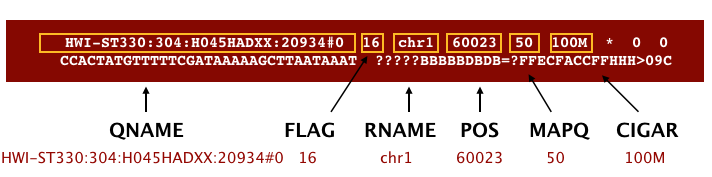
\includegraphics{index_files/mediabag/sam_bam.png}

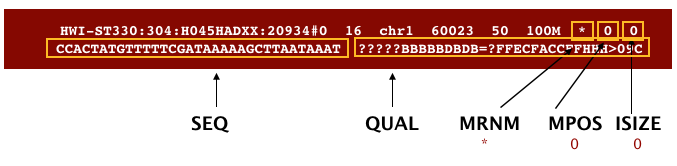
\includegraphics{index_files/mediabag/sam_bam3.png}

We will convert the SAM file to BAM format using the \texttt{samtools}
program (Li et al. 2009) with the \texttt{view} command and tell this
command that the input is in SAM format (\texttt{-S}) and to output BAM
format (\texttt{-b}):

\begin{Shaded}
\begin{Highlighting}[]
\ExtensionTok{$}\NormalTok{ source package /tsl/software/testing/bin/samtools{-}1.9}
\ExtensionTok{$}\NormalTok{ samtools view }\AttributeTok{{-}S} \AttributeTok{{-}b}\NormalTok{ results/sam/SRR2584866.aligned.sam }\OperatorTok{\textgreater{}}\NormalTok{ results/bam/SRR2584866.aligned.bam}
\ExtensionTok{[samopen]}\NormalTok{ SAM header is present: 1 sequences.}
\end{Highlighting}
\end{Shaded}

\hypertarget{sort-bam-file-by-coordinates}{%
\subsection{Sort BAM file by
coordinates}\label{sort-bam-file-by-coordinates}}

Next we sort the BAM file using the \texttt{sort} command from
\texttt{samtools}. \texttt{-o} tells the command where to write the
output. Our files are pretty small, so we will not see this output. If
you run the workflow with larger files, you will see something like
this:

\begin{Shaded}
\begin{Highlighting}[]
\ExtensionTok{$}\NormalTok{ samtools sort }\AttributeTok{{-}o}\NormalTok{ results/bam/SRR2584866.aligned.sorted.bam results/bam/SRR2584866.aligned.bam}
\ExtensionTok{[bam\_sort\_core]}\NormalTok{ merging from 2 files...}
\end{Highlighting}
\end{Shaded}

SAM/BAM files can be sorted in multiple ways, e.g.~by location of
alignment on the chromosome, by read name, etc. It is important to be
aware that different alignment tools will output differently sorted
SAM/BAM, and different downstream tools require differently sorted
alignment files as input.

You can use \texttt{samtools} to learn more about this BAM file as well.

\begin{Shaded}
\begin{Highlighting}[]
\ExtensionTok{$}\NormalTok{ samtools flagstat results/bam/SRR2584866.aligned.sorted.bam}
\end{Highlighting}
\end{Shaded}

This will give you the following statistics about your sorted bam file:

\begin{verbatim}
351169 + 0 in total (QC-passed reads + QC-failed reads)
0 + 0 secondary
1169 + 0 supplementary
0 + 0 duplicates
351103 + 0 mapped (99.98% : N/A)
350000 + 0 paired in sequencing
175000 + 0 read1
175000 + 0 read2
346688 + 0 properly paired (99.05% : N/A)
349876 + 0 with itself and mate mapped
58 + 0 singletons (0.02% : N/A)
0 + 0 with mate mapped to a different chr
0 + 0 with mate mapped to a different chr (mapQ>=5)
\end{verbatim}

\hypertarget{variant-calling}{%
\section{Variant calling}\label{variant-calling}}

A variant call is a conclusion that there is a nucleotide difference
vs.~some reference at a given position in an individual genome or
transcriptome, often referred to as a Single Nucleotide Variant (SNV).
The call is usually accompanied by an estimate of variant frequency and
some measure of confidence. Similar to other steps in this workflow,
there are a number of tools available for variant calling. In this
workshop we will be using \texttt{bcftools}, but there are a few things
we need to do before actually calling the variants.

\begin{Shaded}
\begin{Highlighting}[]
\ExtensionTok{$}\NormalTok{ source package /tsl/software/testing/bin/bcftools{-}1.9}
\ExtensionTok{loaded}\NormalTok{ /tsl/software/testing/bin/bcftools{-}1.9}
\end{Highlighting}
\end{Shaded}

\hypertarget{step-1-calculate-the-read-coverage-of-positions-in-the-genome}{%
\subsection{Step 1: Calculate the read coverage of positions in the
genome}\label{step-1-calculate-the-read-coverage-of-positions-in-the-genome}}

Do the first pass on variant calling by counting read coverage with
bcftools. We will use the command mpileup. The flag -O b tells bcftools
to generate a bcf format output file, -o specifies where to write the
output file, and -f flags the path to the reference genome:

\begin{Shaded}
\begin{Highlighting}[]
\ExtensionTok{$}\NormalTok{ bcftools mpileup }\AttributeTok{{-}O}\NormalTok{ b }\AttributeTok{{-}o}\NormalTok{ results/bcf/SRR2584866\_raw.bcf }\DataTypeTok{\textbackslash{}}
\NormalTok{{-}f data/ref\_genome/ecoli\_rel606.fasta results/bam/SRR2584866.aligned.sorted.bam}
\ExtensionTok{[mpileup]}\NormalTok{ 1 samples in 1 input files}
\ExtensionTok{...}
\end{Highlighting}
\end{Shaded}

It should take less than 1 minute to finish.

We have now generated a file with coverage information for every base.

\hypertarget{step-2-detect-the-single-nucleotide-variants-snvs}{%
\subsection{Step 2: Detect the single nucleotide variants
(SNVs)}\label{step-2-detect-the-single-nucleotide-variants-snvs}}

Identify SNVs using \texttt{bcftools\ call}. We have to specify ploidy
with the flag \texttt{-\/-ploidy}, which is one for the haploid \emph{E.
coli}. \texttt{-m} allows for multi-allelic and rare-variant calling,
\texttt{-v} tells the program to output variant sites only (not every
site in the genome), and \texttt{-o} specifies where to write the output
file:

\begin{Shaded}
\begin{Highlighting}[]
\ExtensionTok{$}\NormalTok{ bcftools call }\AttributeTok{{-}{-}ploidy}\NormalTok{ 1 }\AttributeTok{{-}m} \AttributeTok{{-}v} \AttributeTok{{-}o}\NormalTok{ results/vcf/SRR2584866\_variants.vcf results/bcf/SRR2584866\_raw.bcf }
\end{Highlighting}
\end{Shaded}

\hypertarget{step-3-filter-and-report-the-snv-variants-in-variant-calling-format-vcf}{%
\subsection{Step 3: Filter and report the SNV variants in variant
calling format
(VCF)}\label{step-3-filter-and-report-the-snv-variants-in-variant-calling-format-vcf}}

Filter the SNVs for the final output in VCF format, using
\texttt{vcfutils.pl}:

\begin{Shaded}
\begin{Highlighting}[]
\ExtensionTok{$}\NormalTok{ vcfutils.pl varFilter results/vcf/SRR2584866\_variants.vcf  }\OperatorTok{\textgreater{}}\NormalTok{ results/vcf/SRR2584866\_final\_variants.vcf}
\end{Highlighting}
\end{Shaded}

\hypertarget{explore-the-vcf-format}{%
\section{Explore the VCF format}\label{explore-the-vcf-format}}

\begin{Shaded}
\begin{Highlighting}[]
\ExtensionTok{$}\NormalTok{ less }\AttributeTok{{-}S}\NormalTok{ results/vcf/SRR2584866\_final\_variants.vcf}
\end{Highlighting}
\end{Shaded}

You will see the header (which describes the format), the time and date
the file was created, the version of \texttt{bcftools} that was used,
the command line parameters used, and some additional information:

\begin{verbatim}
##fileformat=VCFv4.2
##FILTER=<ID=PASS,Description="All filters passed">
##bcftoolsVersion=1.8+htslib-1.8
##bcftoolsCommand=mpileup -O b -o results/bcf/SRR2584866_raw.bcf -f data/ref_genome/ecoli_rel606.fasta results/bam/SRR2584866.aligned.sorted.bam
##reference=file://data/ref_genome/ecoli_rel606.fasta
##contig=<ID=CP000819.1,length=4629812>
##ALT=<ID=*,Description="Represents allele(s) other than observed.">
##INFO=<ID=INDEL,Number=0,Type=Flag,Description="Indicates that the variant is an INDEL.">
##INFO=<ID=IDV,Number=1,Type=Integer,Description="Maximum number of reads supporting an indel">
##INFO=<ID=IMF,Number=1,Type=Float,Description="Maximum fraction of reads supporting an indel">
##INFO=<ID=DP,Number=1,Type=Integer,Description="Raw read depth">
##INFO=<ID=VDB,Number=1,Type=Float,Description="Variant Distance Bias for filtering splice-site artefacts in RNA-seq data (bigger is better)",Version=
##INFO=<ID=RPB,Number=1,Type=Float,Description="Mann-Whitney U test of Read Position Bias (bigger is better)">
##INFO=<ID=MQB,Number=1,Type=Float,Description="Mann-Whitney U test of Mapping Quality Bias (bigger is better)">
##INFO=<ID=BQB,Number=1,Type=Float,Description="Mann-Whitney U test of Base Quality Bias (bigger is better)">
##INFO=<ID=MQSB,Number=1,Type=Float,Description="Mann-Whitney U test of Mapping Quality vs Strand Bias (bigger is better)">
##INFO=<ID=SGB,Number=1,Type=Float,Description="Segregation based metric.">
##INFO=<ID=MQ0F,Number=1,Type=Float,Description="Fraction of MQ0 reads (smaller is better)">
##FORMAT=<ID=PL,Number=G,Type=Integer,Description="List of Phred-scaled genotype likelihoods">
##FORMAT=<ID=GT,Number=1,Type=String,Description="Genotype">
##INFO=<ID=ICB,Number=1,Type=Float,Description="Inbreeding Coefficient Binomial test (bigger is better)">
##INFO=<ID=HOB,Number=1,Type=Float,Description="Bias in the number of HOMs number (smaller is better)">
##INFO=<ID=AC,Number=A,Type=Integer,Description="Allele count in genotypes for each ALT allele, in the same order as listed">
##INFO=<ID=AN,Number=1,Type=Integer,Description="Total number of alleles in called genotypes">
##INFO=<ID=DP4,Number=4,Type=Integer,Description="Number of high-quality ref-forward , ref-reverse, alt-forward and alt-reverse bases">
##INFO=<ID=MQ,Number=1,Type=Integer,Description="Average mapping quality">
##bcftools_callVersion=1.8+htslib-1.8
##bcftools_callCommand=call --ploidy 1 -m -v -o results/bcf/SRR2584866_variants.vcf results/bcf/SRR2584866_raw.bcf; Date=Tue Oct  9 18:48:10 2018
\end{verbatim}

Followed by information on each of the variations observed:

\begin{verbatim}
#CHROM  POS     ID      REF     ALT     QUAL    FILTER  INFO    FORMAT  results/bam/SRR2584866.aligned.sorted.bam
CP000819.1      1521    .       C       T       207     .       DP=9;VDB=0.993024;SGB=-0.662043;MQSB=0.974597;MQ0F=0;AC=1;AN=1;DP4=0,0,4,5;MQ=60
CP000819.1      1612    .       A       G       225     .       DP=13;VDB=0.52194;SGB=-0.676189;MQSB=0.950952;MQ0F=0;AC=1;AN=1;DP4=0,0,6,5;MQ=60
CP000819.1      9092    .       A       G       225     .       DP=14;VDB=0.717543;SGB=-0.670168;MQSB=0.916482;MQ0F=0;AC=1;AN=1;DP4=0,0,7,3;MQ=60
CP000819.1      9972    .       T       G       214     .       DP=10;VDB=0.022095;SGB=-0.670168;MQSB=1;MQ0F=0;AC=1;AN=1;DP4=0,0,2,8;MQ=60      GT:PL
CP000819.1      10563   .       G       A       225     .       DP=11;VDB=0.958658;SGB=-0.670168;MQSB=0.952347;MQ0F=0;AC=1;AN=1;DP4=0,0,5,5;MQ=60
CP000819.1      22257   .       C       T       127     .       DP=5;VDB=0.0765947;SGB=-0.590765;MQSB=1;MQ0F=0;AC=1;AN=1;DP4=0,0,2,3;MQ=60      GT:PL
CP000819.1      38971   .       A       G       225     .       DP=14;VDB=0.872139;SGB=-0.680642;MQSB=1;MQ0F=0;AC=1;AN=1;DP4=0,0,4,8;MQ=60      GT:PL
CP000819.1      42306   .       A       G       225     .       DP=15;VDB=0.969686;SGB=-0.686358;MQSB=1;MQ0F=0;AC=1;AN=1;DP4=0,0,5,9;MQ=60      GT:PL
CP000819.1      45277   .       A       G       225     .       DP=15;VDB=0.470998;SGB=-0.680642;MQSB=0.95494;MQ0F=0;AC=1;AN=1;DP4=0,0,7,5;MQ=60
CP000819.1      56613   .       C       G       183     .       DP=12;VDB=0.879703;SGB=-0.676189;MQSB=1;MQ0F=0;AC=1;AN=1;DP4=0,0,8,3;MQ=60      GT:PL
CP000819.1      62118   .       A       G       225     .       DP=19;VDB=0.414981;SGB=-0.691153;MQSB=0.906029;MQ0F=0;AC=1;AN=1;DP4=0,0,8,10;MQ=59
CP000819.1      64042   .       G       A       225     .       DP=18;VDB=0.451328;SGB=-0.689466;MQSB=1;MQ0F=0;AC=1;AN=1;DP4=0,0,7,9;MQ=60      GT:PL
\end{verbatim}

This is a lot of information, so let's take some time to make sure we
understand our output.

The first few columns represent the information we have about a
predicted variation.

\begin{longtable}[]{@{}
  >{\raggedright\arraybackslash}p{(\columnwidth - 2\tabcolsep) * \real{0.2917}}
  >{\raggedright\arraybackslash}p{(\columnwidth - 2\tabcolsep) * \real{0.7083}}@{}}
\toprule\noalign{}
\begin{minipage}[b]{\linewidth}\raggedright
column
\end{minipage} & \begin{minipage}[b]{\linewidth}\raggedright
info
\end{minipage} \\
\midrule\noalign{}
\endhead
\bottomrule\noalign{}
\endlastfoot
CHROM & contig location where the variation occurs \\
POS & position within the contig where the variation occurs \\
ID & a \texttt{.} until we add annotation information \\
REF & reference genotype (forward strand) \\
ALT & sample genotype (forward strand) \\
QUAL & Phred-scaled probability that the observed variant exists at this
site (higher is better) \\
FILTER & a \texttt{.} if no quality filters have been applied, PASS if a
filter is passed, or the name of the filters this variant failed \\
\end{longtable}

In an ideal world, the information in the \texttt{QUAL} column would be
all we needed to filter out bad variant calls. However, in reality we
need to filter on multiple other metrics.

The last two columns contain the genotypes and can be tricky to decode.

\begin{longtable}[]{@{}ll@{}}
\toprule\noalign{}
column & info \\
\midrule\noalign{}
\endhead
\bottomrule\noalign{}
\endlastfoot
FORMAT & lists in order the metrics presented in the final column \\
results & lists the values associated with those metrics in order \\
\end{longtable}

For our file, the metrics presented are GT:PL:GQ.

\begin{longtable}[]{@{}
  >{\raggedright\arraybackslash}p{(\columnwidth - 2\tabcolsep) * \real{0.2778}}
  >{\raggedright\arraybackslash}p{(\columnwidth - 2\tabcolsep) * \real{0.7222}}@{}}
\toprule\noalign{}
\begin{minipage}[b]{\linewidth}\raggedright
metric
\end{minipage} & \begin{minipage}[b]{\linewidth}\raggedright
definition
\end{minipage} \\
\midrule\noalign{}
\endhead
\bottomrule\noalign{}
\endlastfoot
AD, DP & the depth per allele by sample and coverage \\
GT & the genotype for the sample at this loci. For a diploid organism,
the GT field indicates the two alleles carried by the sample, encoded by
a 0 for the REF allele, 1 for the first ALT allele, 2 for the second ALT
allele, etc. A 0/0 means homozygous reference, 0/1 is heterozygous, and
1/1 is homozygous for the alternate allele. \\
PL & the likelihoods of the given genotypes \\
GQ & the Phred-scaled confidence for the genotype \\
\end{longtable}

The Broad Institute's
\href{https://www.broadinstitute.org/gatk/guide/article?id=1268}{VCF
guide} is an excellent place to learn more about the VCF file format.

\begin{tcolorbox}[enhanced jigsaw, toptitle=1mm, breakable, bottomrule=.15mm, colback=white, toprule=.15mm, opacityback=0, bottomtitle=1mm, coltitle=black, opacitybacktitle=0.6, rightrule=.15mm, colframe=quarto-callout-caution-color-frame, titlerule=0mm, colbacktitle=quarto-callout-caution-color!10!white, title={Exercise}, left=2mm, leftrule=.75mm, arc=.35mm]

Use the \texttt{grep} and \texttt{wc} commands you have learned to
assess how many variants are in the vcf file.

\end{tcolorbox}

\begin{tcolorbox}[enhanced jigsaw, toptitle=1mm, breakable, bottomrule=.15mm, colback=white, toprule=.15mm, opacityback=0, bottomtitle=1mm, coltitle=black, opacitybacktitle=0.6, rightrule=.15mm, colframe=quarto-callout-caution-color-frame, titlerule=0mm, colbacktitle=quarto-callout-caution-color!10!white, title={Solution}, left=2mm, leftrule=.75mm, arc=.35mm]

\begin{Shaded}
\begin{Highlighting}[]
\ExtensionTok{$}\NormalTok{ grep }\AttributeTok{{-}v} \StringTok{"\#"}\NormalTok{ results/vcf/SRR2584866\_final\_variants.vcf }\KeywordTok{|} \FunctionTok{wc} \AttributeTok{{-}l}
\ExtensionTok{765}
\end{Highlighting}
\end{Shaded}

There are 765 variants in this file.

\end{tcolorbox}

\hypertarget{visualize-and-assess-the-alignment}{%
\section{Visualize and assess the
alignment}\label{visualize-and-assess-the-alignment}}

It is often instructive to look at your data in a genome browser.
Visualization will allow you to get a ``feel'' for the data, as well as
detecting abnormalities and problems. Also, exploring the data in such a
way may give you ideas for further analyses. As such, visualization
tools are useful for exploratory analysis. In this lesson we will
describe two different tools for visualization: a light-weight
command-line based one and the Broad Institute's Integrative Genomics
Viewer (IGV) which requires software installation and transfer of files.

In order for us to visualize the alignment files, we will need to index
the BAM file using \texttt{samtools}:

\begin{verbatim}
$ samtools index results/bam/SRR2584866.aligned.sorted.bam
\end{verbatim}

\hypertarget{visualization-with-tview}{%
\subsection{Visualization with tview}\label{visualization-with-tview}}

\href{http://www.htslib.org/}{Samtools} implements a very simple text
alignment viewer based on the GNU \texttt{ncurses} library, called
\texttt{tview}. This alignment viewer works with short indels and shows
\href{http://maq.sourceforge.net/}{MAQ} consensus. It uses different
colors to display mapping quality or base quality, subjected to users'
choice. Samtools viewer is known to work with a 130 GB alignment
swiftly. Due to its text interface, displaying alignments over network
is also very fast.

In order to visualize our mapped reads, we use \texttt{tview}, giving it
the sorted bam file and the reference file:

\begin{Shaded}
\begin{Highlighting}[]
\ExtensionTok{$}\NormalTok{ samtools tview results/bam/SRR2584866.aligned.sorted.bam data/ref\_genome/ecoli\_rel606.fasta}
\end{Highlighting}
\end{Shaded}

\begin{verbatim}
1         11        21        31        41        51        61        71        81        91        101       111       121
AGCTTTTCATTCTGACTGCAACGGGCAATATGTCTCTGTGTGGATTAAAAAAAGAGTGTCTGATAGCAGCTTCTGAACTGGTTACCTGCCGTGAGTAAATTAAAATTTTATTGACTTAGGTCACTAAATAC
..................................................................................................................................
,,,,,,,,,,,,,,,,,,,,,,,,,,,,,,,,,,,, ..................N................. ,,,,,,,,,,,,,,,,,,,,,,,,,,,,,,,,........................
,,,,,,,,,,,,,,,,,,,,,,,,,,,,,,,,,,, ..................N................. ,,,,,,,,,,,,,,,,,,,,,,,,,,,.............................
...................................,g,,,,,,,,,,,,,,,,,,,,,,,,,,,,,,,,,  ....................................   ................
,,,,,,,,,,,,,,,,,,,,,,,,,,,,,,,,,,,....................................   ....................................      ,,,,,,,,,,
,,,,,,,,,,,,,,,,,,,,,,,,,,,,,,,,,,,,  ....................................  ,,a,,,,,,,,,,,,,,,,,,,,,,,,,,,,,     .......
,,,,,,,,,,,,,,,,,,,,,,,,,,,,,,, .............................  ,,,,,,,,,,,,,,,,,g,,,,,    ,,,,,,,,,,,,,,,,,,,,,,,,,,,,
,,,,,,,,,,,,,,,,,,,,,,,,,,,,,,,,,,,  ...........................T.......   ,,,,,,,,,,,,,,,,,,,,,,,c,          ......
......................... ................................   ,g,,,,,,,,,,,,,,,,,,,      ...........................
,,,,,,,,,,,,,,,,,,,,, ,,,,,,,,,,,,,,,,,,,,,,,,,,,,,,, ,,,,,,,,,,,,,,,,,,,,,,,,,,,       ..........................
,,,,,,,,,,,,,,,,,,,,,,,,,,,,,,,,,,,   ................................T..  ..............................   ,,,,,,
...........................       ,,,,,,g,,,,,,,,,,,,,,,,,   ....................................         ,,,,,,
,,,,,,,,,,,,,,,,,,,,,,,,,, ....................................  ...................................        ....
....................................  ........................  ,,,,,,,,,,,,,,,,,,,,,,,,,,,,,,,,,,,,      ....
,,,,,,,,,,,,,,,,,,,,,,,,,,,,,,,,,,,,   ,,,,,,,,,,,,,,,,,,,,,,,,,,,,,,,,,,,,  ,,,,,,,,,,,,,,,,,,,,,,,,,,,,,,,,,
........................            .................................. .............................     ....
,,,,,,,,,,,,,,,,,,,,,,,,,,,,,,,,,,,,   ....................................        ..........................
...............................       ,,,,,,,,,,,,,,,,,,,,,,,,,,,,,,,, ....................................
...................................  ,,,,,,,,,,,,,,,,,,,,,,,,,,,,,,,,  ,,,,,,,,,,,,,,,,,,,,,,,,,,,,,,,,,,,
,,,,,,,,,,,,,,,,,,,,,,,,,,,,,,,,,,,, ,,,,,,,,,,,,,,,,,,,,,,,,,,,,,,,,,,  ..................................
.................................... ,,,,,,,,,,,,,,,,,,a,,,,,,,,,,,,,,,,,        ,,,,,,,,,,,,,,,,,,,,,,,,,
,,,,,,,,,,,,,,,,,,,,,,,,,,,,,,,,,,,  ............................ ,,,,,,,,,,,,,,,,,,,,,,,,,,,,,,,,,,,,
\end{verbatim}

The first line of output shows the genome coordinates in our reference
genome. The second line shows the reference genome sequence. The third
line shows the consensus sequence determined from the sequence reads. A
\texttt{.} indicates a match to the reference sequence, so we can see
that the consensus from our sample matches the reference in most
locations. That is good! If that was not the case, we should probably
reconsider our choice of reference.

Below the horizontal line, we can see all of the reads in our sample
aligned with the reference genome. Only positions where the called base
differs from the reference are shown. You can use the arrow keys on your
keyboard to scroll or type \texttt{?} for a help menu. To navigate to a
specific position, type \texttt{g}. A dialogue box will appear. In this
box, type the name of the ``chromosome'' followed by a colon and the
position of the variant you would like to view (e.g.~for this sample,
type \texttt{CP000819.1:50} to view the 50th base. Type
\texttt{Ctrl\^{}C} or \texttt{q} to exit \texttt{tview}.

\begin{tcolorbox}[enhanced jigsaw, toptitle=1mm, breakable, bottomrule=.15mm, colback=white, toprule=.15mm, opacityback=0, bottomtitle=1mm, coltitle=black, opacitybacktitle=0.6, rightrule=.15mm, colframe=quarto-callout-caution-color-frame, titlerule=0mm, colbacktitle=quarto-callout-caution-color!10!white, title={Exercise}, left=2mm, leftrule=.75mm, arc=.35mm]

Visualize the alignment of the reads for our SRR2584866 sample. What
variant is present at position 4377265? What is the canonical nucleotide
in that position?

\end{tcolorbox}

\begin{tcolorbox}[enhanced jigsaw, toptitle=1mm, breakable, bottomrule=.15mm, colback=white, toprule=.15mm, opacityback=0, bottomtitle=1mm, coltitle=black, opacitybacktitle=0.6, rightrule=.15mm, colframe=quarto-callout-caution-color-frame, titlerule=0mm, colbacktitle=quarto-callout-caution-color!10!white, title={Solution}, left=2mm, leftrule=.75mm, arc=.35mm]

\begin{Shaded}
\begin{Highlighting}[]
\ExtensionTok{$}\NormalTok{ samtools tview \textasciitilde{}/dc\_workshop/results/bam/SRR2584866.aligned.sorted.bam \textasciitilde{}/dc\_workshop/data/ref\_genome/ecoli\_rel606.fasta}
\end{Highlighting}
\end{Shaded}

Then type \texttt{g}. In the dialogue box, type
\texttt{CP000819.1:4377265}. \texttt{G} is the variant. \texttt{A} is
canonical. This variant possibly changes the phenotype of this sample to
hypermutable. It occurs in the gene \emph{mutL}, which controls DNA
mismatch repair.

\end{tcolorbox}

\hypertarget{visualization-with-igv}{%
\subsection{Visualization with IGV}\label{visualization-with-igv}}

\href{http://www.broadinstitute.org/igv/}{IGV} is a stand-alone browser,
which has the advantage of being installed locally and providing fast
access. Web-based genome browsers, like
\href{http://www.ensembl.org/index.html}{Ensembl} or the
\href{https://genome.ucsc.edu/}{UCSC browser}, are slower, but provide
more functionality. They not only allow for more polished and flexible
visualization, but also provide easy access to a wealth of annotations
and external data sources. This makes it straightforward to relate your
data with information about repeat regions, known genes, epigenetic
features or areas of cross-species conservation, to name just a few.

In order to use IGV, we will need to transfer some files to our local
machine. We know how to do this with the Windows navigation system. Open
a new tab in your terminal window and create a new folder. We will put
this folder on our Desktop for demonstration purposes, but in general
you should avoid proliferating folders and files on your Desktop and
instead organize files within a directory structure like we have been
using in our \texttt{dc\_workshop} directory. Now we will transfer our
files to that new local directory.

Next, we need to open the IGV software. If you have not done so already,
you can download IGV from the
\href{https://www.broadinstitute.org/software/igv/download}{Broad
Institute's software page}, double-click the \texttt{.zip} file to unzip
it, and then drag the program into your Applications folder.

\begin{enumerate}
\def\labelenumi{\arabic{enumi}.}
\item
  Open IGV.

  \begin{tcolorbox}[enhanced jigsaw, toptitle=1mm, breakable, bottomrule=.15mm, colback=white, toprule=.15mm, opacityback=0, bottomtitle=1mm, coltitle=black, opacitybacktitle=0.6, rightrule=.15mm, colframe=quarto-callout-tip-color-frame, titlerule=0mm, colbacktitle=quarto-callout-tip-color!10!white, title=\textcolor{quarto-callout-tip-color}{\faLightbulb}\hspace{0.5em}{Tip}, left=2mm, leftrule=.75mm, arc=.35mm]

  IGV is already installed on your computer and you can find the icon
  shortcut on your Desktop.

  \end{tcolorbox}
\item
  Load our reference genome file (\texttt{ecoli\_rel606.fasta}) into IGV
  using the \textbf{``Load Genomes from File\ldots{}''} option under the
  \textbf{``Genomes''} pull-down menu.

  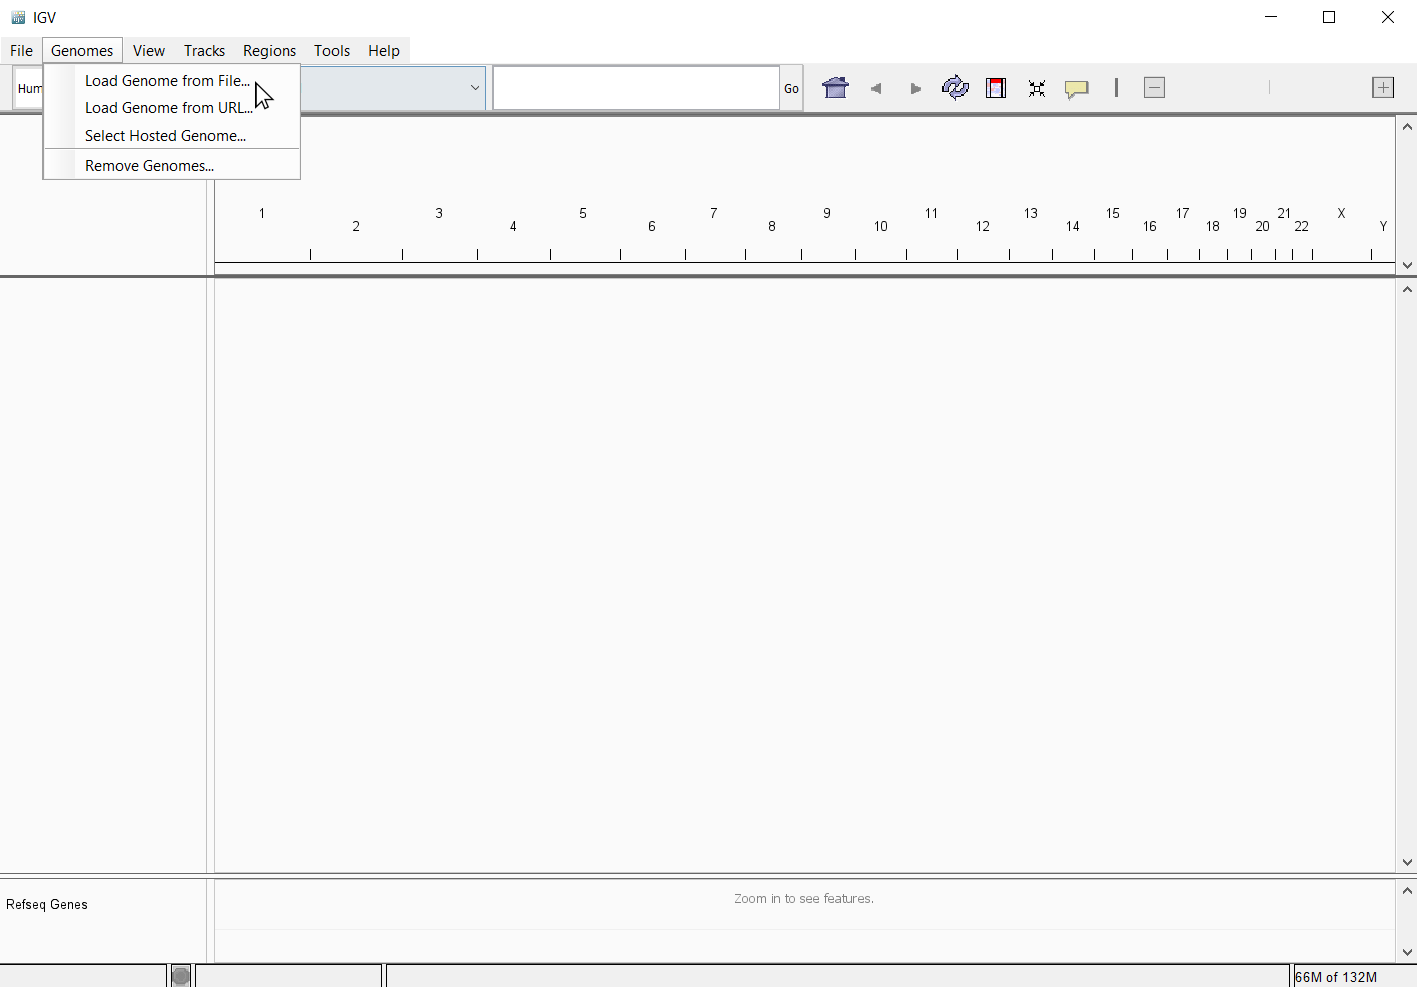
\includegraphics{images/igv-load-genomes-from-file.png}

  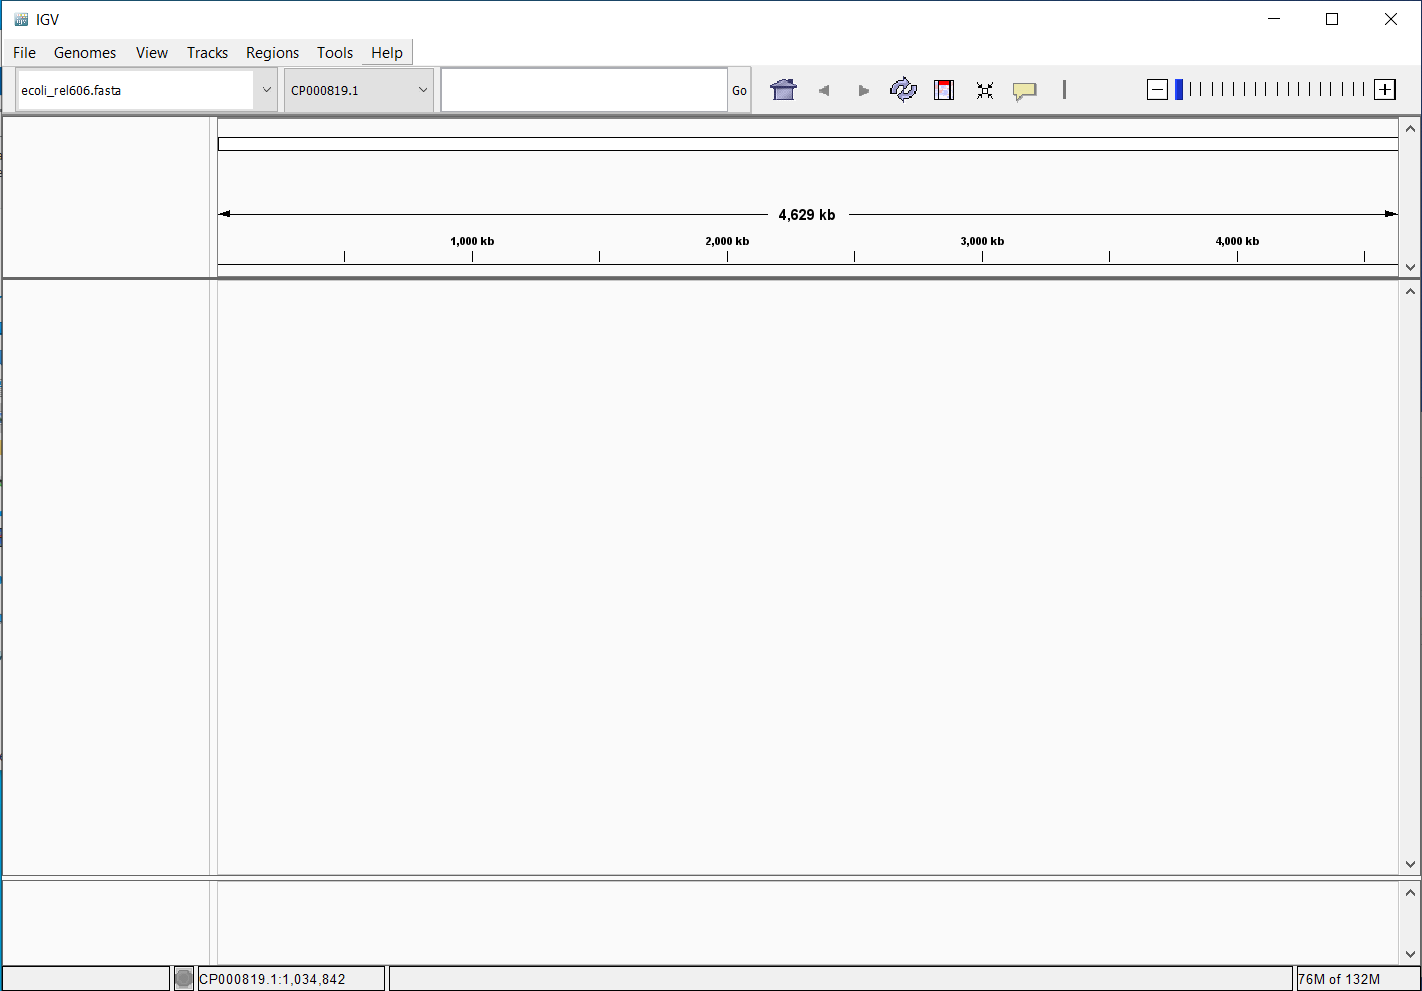
\includegraphics{images/igv-genome-loaded.png}
\item
  Load our BAM file (\texttt{SRR2584866.aligned.sorted.bam}) using the
  \textbf{``Load from File\ldots{}''} option under the \textbf{``File''}
  pull-down menu.

  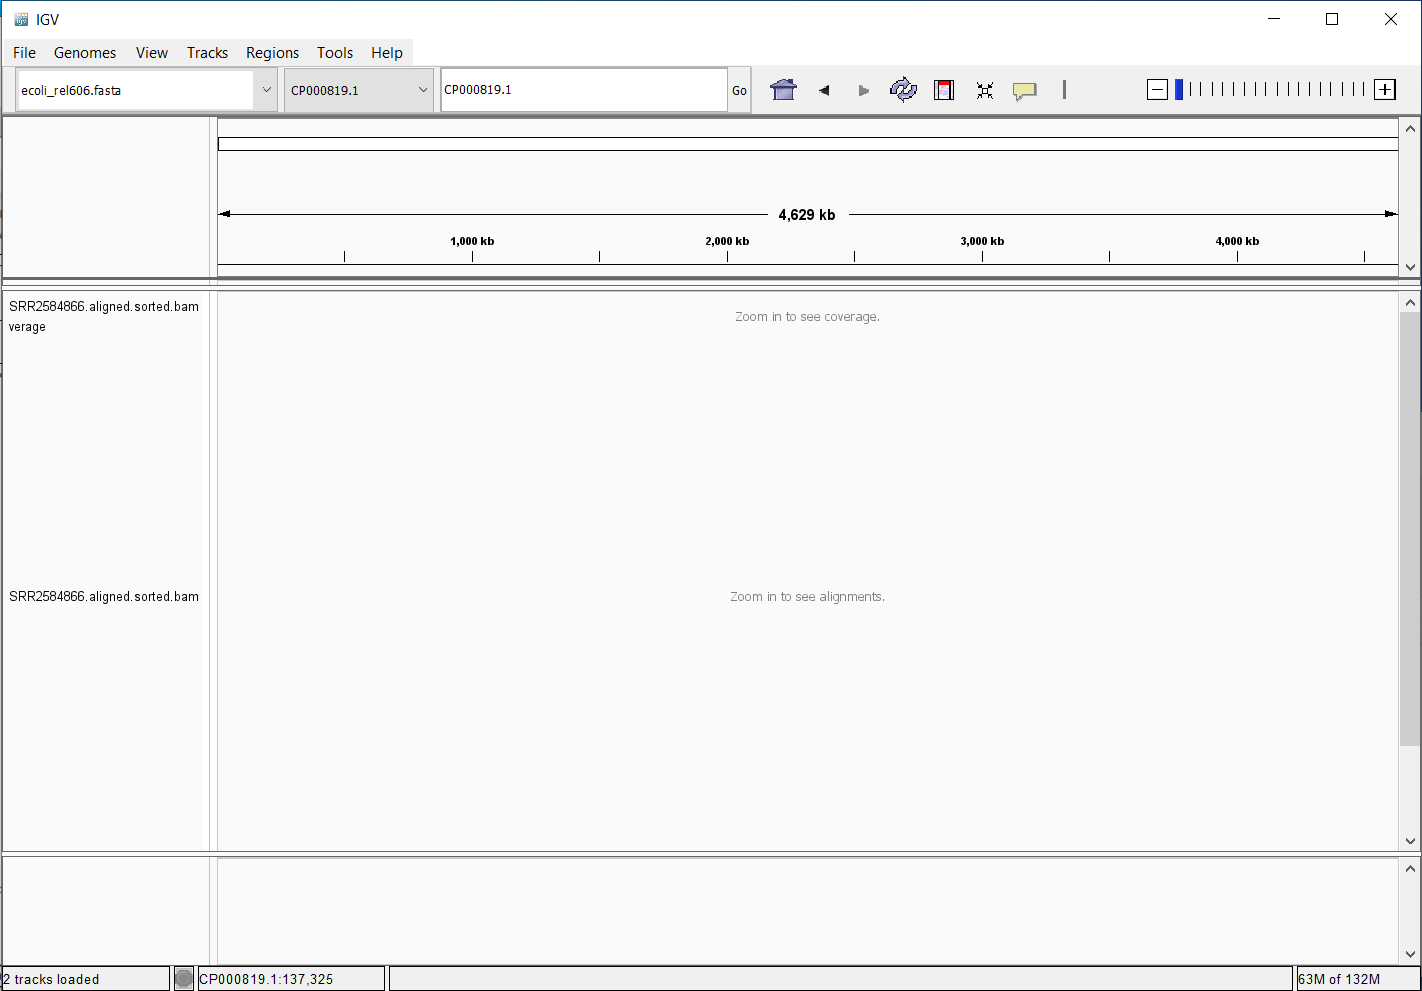
\includegraphics{images/igv-bam-loaded.png}
\item
  Do the same with our VCF file
  (\texttt{SRR2584866\_final\_variants.vcf}).

  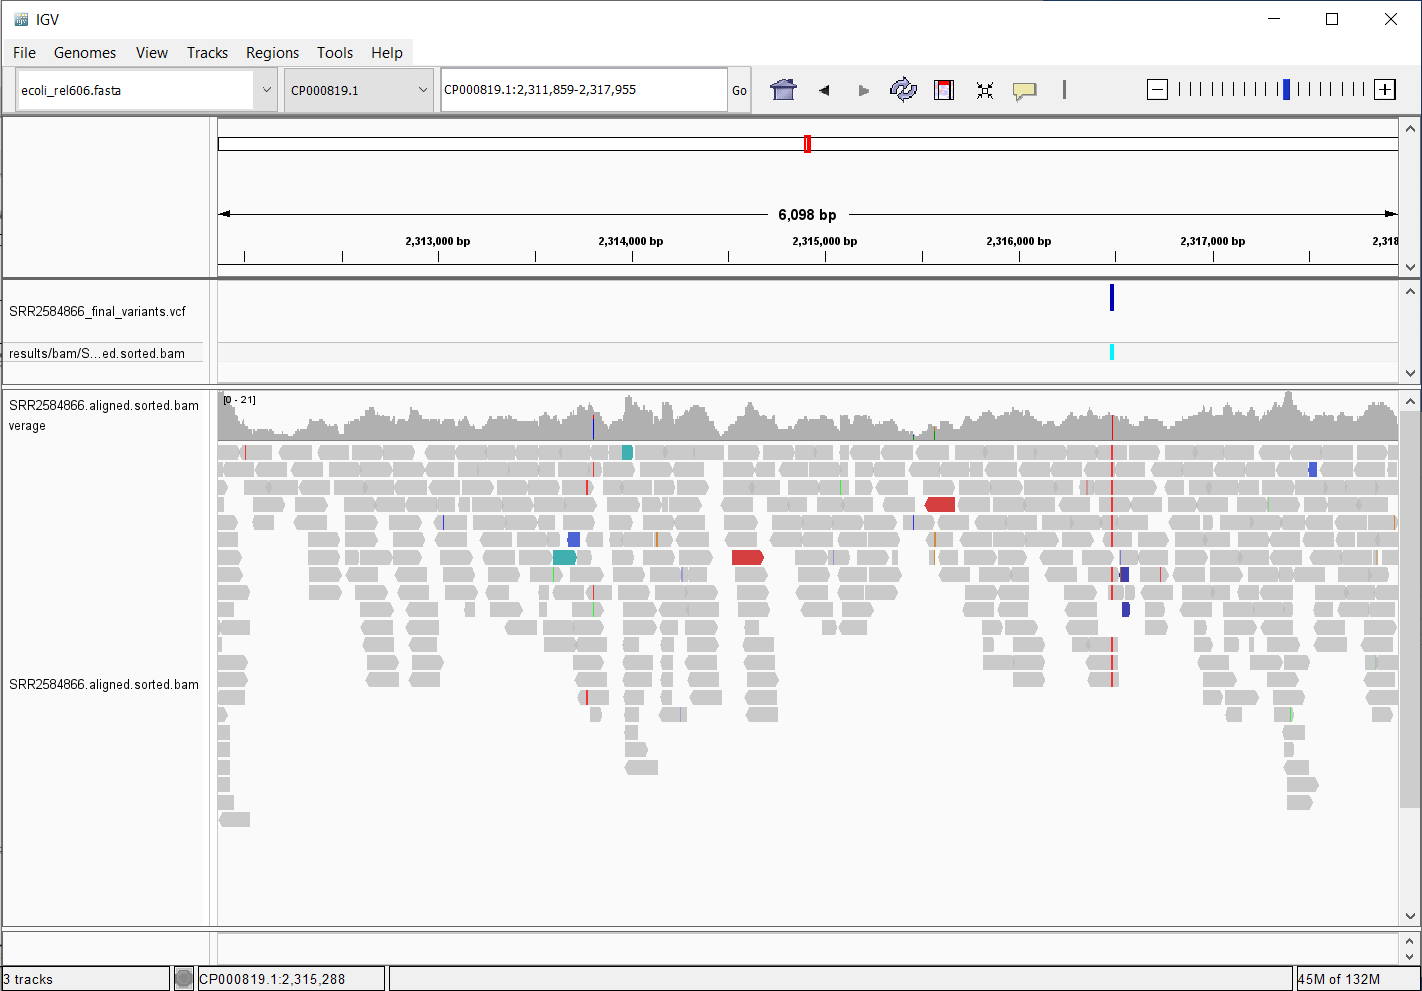
\includegraphics{images/igv-vcf-loaded.png}
\end{enumerate}

There should be two tracks: one corresponding to our BAM file and the
other for our VCF file.

In the \textbf{VCF track}, each bar across the top of the plot shows the
allele fraction for a single locus. The second bar shows the genotypes
for each locus in each \emph{sample}. We only have one sample called
here, so we only see a single line.

\begin{itemize}
\item
  Dark blue = heterozygous,
\item
  Cyan = homozygous variant,
\item
  Grey = reference.
\item
  Filtered entries are transparent.
\end{itemize}

Zoom in to inspect variants you see in your filtered VCF file to become
more familiar with IGV. See how quality information corresponds to
alignment information at those loci. Use
\href{http://software.broadinstitute.org/software/igv/AlignmentData}{this
website} and the links therein to understand how IGV colors the
alignments.

Now that we have run through our workflow for a single sample, we want
to repeat this workflow for our other five samples. However, we do not
want to type each of these individual steps again five more times. That
would be very time consuming and error-prone, and would become
impossible as we gathered more and more samples. Luckily, we already
know the tools we need to use to automate this workflow and run it on as
many files as we want using a single line of code. Those tools are:
wildcards, for loops, and bash scripts. We will use all three in the
next lesson.

\hypertarget{summary-3}{%
\section{Summary}\label{summary-3}}

\begin{tcolorbox}[enhanced jigsaw, toptitle=1mm, breakable, bottomrule=.15mm, colback=white, toprule=.15mm, opacityback=0, bottomtitle=1mm, coltitle=black, opacitybacktitle=0.6, rightrule=.15mm, colframe=quarto-callout-important-color-frame, titlerule=0mm, colbacktitle=quarto-callout-important-color!10!white, title=\textcolor{quarto-callout-important-color}{\faExclamation}\hspace{0.5em}{Key points}, left=2mm, leftrule=.75mm, arc=.35mm]

\begin{itemize}
\tightlist
\item
  Bioinformatic command line tools are collections of commands that can
  be used to carry out bioinformatic analyses.
\item
  To use most powerful bioinformatic tools, you will need to use the
  command line.
\item
  There are many different file formats for storing genomics data. It is
  important to understand what type of information is contained in each
  file, and how it was derived.
\end{itemize}

\end{tcolorbox}

\bookmarksetup{startatroot}

\hypertarget{automating-a-variant-calling-workflow}{%
\chapter{Automating a variant calling
workflow}\label{automating-a-variant-calling-workflow}}

\begin{tcolorbox}[enhanced jigsaw, toptitle=1mm, breakable, bottomrule=.15mm, colback=white, toprule=.15mm, opacityback=0, bottomtitle=1mm, coltitle=black, opacitybacktitle=0.6, rightrule=.15mm, colframe=quarto-callout-note-color-frame, titlerule=0mm, colbacktitle=quarto-callout-note-color!10!white, title={⏳ Time}, left=2mm, leftrule=.75mm, arc=.35mm]

\begin{itemize}
\tightlist
\item
  Teaching: 30 min
\item
  Exercises: 15 min
\end{itemize}

\end{tcolorbox}

\begin{tcolorbox}[enhanced jigsaw, toptitle=1mm, breakable, bottomrule=.15mm, colback=white, toprule=.15mm, opacityback=0, bottomtitle=1mm, coltitle=black, opacitybacktitle=0.6, rightrule=.15mm, colframe=quarto-callout-tip-color-frame, titlerule=0mm, colbacktitle=quarto-callout-tip-color!10!white, title={🤔 Question}, left=2mm, leftrule=.75mm, arc=.35mm]

\begin{itemize}
\tightlist
\item
  How can I make my workflow more efficient and less error-prone?
\end{itemize}

\end{tcolorbox}

\begin{tcolorbox}[enhanced jigsaw, toptitle=1mm, breakable, bottomrule=.15mm, colback=white, toprule=.15mm, opacityback=0, bottomtitle=1mm, coltitle=black, opacitybacktitle=0.6, rightrule=.15mm, colframe=quarto-callout-important-color-frame, titlerule=0mm, colbacktitle=quarto-callout-important-color!10!white, title={🎯 Objectives}, left=2mm, leftrule=.75mm, arc=.35mm]

\begin{itemize}
\tightlist
\item
  Write a shell script with multiple variables.
\item
  Incorporate a for loop into a shell script.
\end{itemize}

\end{tcolorbox}

\hypertarget{what-is-a-shell-script}{%
\section{What is a shell script?}\label{what-is-a-shell-script}}

You wrote a simple shell script in a previous lesson that we used to
extract bad reads from our FASTQ files and put them into a new file.

Here is the script you wrote:

\begin{verbatim}
grep -B1 -A2 NNNNNNNNNN *.fastq > scripted_bad_reads.txt

echo "Script finished!"
\end{verbatim}

That script was only two lines long, but shell scripts can be much more
complicated than that and can be used to perform a large number of
operations on one or many files. This saves you the effort of having to
type each of those commands over for each of your data files and makes
your work less error-prone and more reproducible. For example, the
variant calling workflow we just carried out had about eight steps where
we had to type a command into our terminal. Most of these commands were
pretty long. If we wanted to do this for all six of our data files, that
would be forty-eight steps. If we had 50 samples (a more realistic
number), it would be 400 steps! You can see why we want to automate
this.

We have also used \texttt{for} loops in previous lessons to iterate one
or two commands over multiple input files. In these \texttt{for} loops,
the filename was defined as a variable in the \texttt{for} statement,
which enabled you to run the loop on multiple files. We will be using
variable assignments like this in our new shell scripts.

Here is the \texttt{for} loop you wrote for unzipping \texttt{.zip}
files:

\begin{verbatim}
$ for filename in *.zip
> do
> unzip $filename
> done
\end{verbatim}

And here is the one you wrote for running Trimmomatic on all of our
\texttt{.fastq} sample files:

\begin{verbatim}
$ for infile in *_1.fastq.gz
> do
>   base=$(basename ${infile} _1.fastq.gz)
>   trimmomatic PE ${infile} ${base}_2.fastq.gz \
>                ${base}_1.trim.fastq.gz ${base}_1un.trim.fastq.gz \
>                ${base}_2.trim.fastq.gz ${base}_2un.trim.fastq.gz \
>                SLIDINGWINDOW:4:20 MINLEN:25 ILLUMINACLIP:NexteraPE-PE.fa:2:40:15 
> done
\end{verbatim}

Notice that in this \texttt{for} loop, we used two variables,
\texttt{infile}, which was defined in the \texttt{for} statement, and
\texttt{base}, which was created from the filename during each iteration
of the loop.

\begin{tcolorbox}[enhanced jigsaw, toptitle=1mm, breakable, bottomrule=.15mm, colback=white, toprule=.15mm, opacityback=0, bottomtitle=1mm, coltitle=black, opacitybacktitle=0.6, rightrule=.15mm, colframe=quarto-callout-note-color-frame, titlerule=0mm, colbacktitle=quarto-callout-note-color!10!white, title=\textcolor{quarto-callout-note-color}{\faInfo}\hspace{0.5em}{Creating variables}, left=2mm, leftrule=.75mm, arc=.35mm]

Within the Bash shell you can create variables at any time (as we did
above, and during the `for' loop lesson). Assign any name and the value
using the assignment operator: `='. You can check the current definition
of your variable by typing into your script: echo \$variable\_name.

\end{tcolorbox}

In this lesson, we will use two shell scripts to automate the variant
calling analysis: one for FastQC analysis (including creating our
summary file), and a second for the remaining variant calling. To write
a script to run our FastQC analysis, we will take each of the commands
we entered to run FastQC and process the output files and put them into
a single file with a \texttt{.sh} extension. The \texttt{.sh} is not
essential, but serves as a reminder to ourselves and to the computer
that this is a shell script.

\hypertarget{analysing-quality-with-fastqc}{%
\section{Analysing quality with
FastQC}\label{analysing-quality-with-fastqc}}

We will use the command \texttt{touch} to create a new file where we
will write our shell script. We will create this script in a new
directory called \texttt{scripts/}. Previously, we used \texttt{nano} to
create and open a new file. The command \texttt{touch} allows us to
create a new file without opening that file.

\begin{Shaded}
\begin{Highlighting}[]
\ExtensionTok{$}\NormalTok{ mkdir }\AttributeTok{{-}p}\NormalTok{ \textasciitilde{}/dc\_workshop/scripts}
\ExtensionTok{$}\NormalTok{ cd \textasciitilde{}/dc\_workshop/scripts}
\ExtensionTok{$}\NormalTok{ touch read\_qc.sh}
\ExtensionTok{$}\NormalTok{ ls}
\ExtensionTok{read\_qc.sh}
\end{Highlighting}
\end{Shaded}

We now have an empty file called \texttt{read\_qc.sh} in our
\texttt{scripts/} directory. We will now open this file in \texttt{nano}
and start building our script.

\begin{Shaded}
\begin{Highlighting}[]
\ExtensionTok{$}\NormalTok{ nano read\_qc.sh}
\end{Highlighting}
\end{Shaded}

\begin{tcolorbox}[enhanced jigsaw, toptitle=1mm, breakable, bottomrule=.15mm, colback=white, toprule=.15mm, opacityback=0, bottomtitle=1mm, coltitle=black, opacitybacktitle=0.6, rightrule=.15mm, colframe=quarto-callout-warning-color-frame, titlerule=0mm, colbacktitle=quarto-callout-warning-color!10!white, title=\textcolor{quarto-callout-warning-color}{\faExclamationTriangle}\hspace{0.5em}{Warning}, left=2mm, leftrule=.75mm, arc=.35mm]

Enter the following pieces of code into your shell script using
\texttt{nano}, not into your terminal prompt (with \texttt{\$}).

\end{tcolorbox}

Our first line will ensure that our script will exit if an error occurs,
and is a good idea to include at the beginning of your scripts. The
second line will move us into the \texttt{untrimmed\_fastq/} directory
when we run our script. Then we load the software needed.

\begin{verbatim}
set -e
cd ~/dc_workshop/data/untrimmed_fastq/

source package /nbi/software/production/bin/fastqc-0.11.8
source package /nbi/software/production/bin/trimmomatic-0.39
\end{verbatim}

These next two lines will give us a status message to tell us that we
are currently running FastQC, then will run FastQC on all of the files
in our current directory with a \texttt{.fastq} extension.

\begin{verbatim}
echo "Running FastQC ..."
fastqc *.fastq*
\end{verbatim}

Our next line will create a new directory to hold our FastQC output
files. Here we are using the \texttt{-p} option for \texttt{mkdir}
again. It is a good idea to use this option in your shell scripts to
avoid running into errors if you do not have the directory structure you
think you do.

\begin{verbatim}
mkdir -p ~/dc_workshop/results/fastqc_untrimmed_reads
\end{verbatim}

Our next three lines first give us a status message to tell us we are
saving the results from FastQC, then moves all of the files with a
\texttt{.zip} or a \texttt{.html} extension to the directory we just
created for storing our FastQC results.

\begin{verbatim}
echo "Saving FastQC results…" 
mv .zip ~/dc_workshop/results/fastqc_untrimmed_reads/ 
mv .html ~/dc_workshop/results/fastqc_untrimmed_reads/
\end{verbatim}

The next line moves us to the results directory where we have stored our
output.

\begin{verbatim}
cd ~/dc_workshop/results/fastqc_untrimmed_reads/
\end{verbatim}

The next five lines should look very familiar. First we give ourselves a
status message to tell us that we are unzipping our ZIP files. Then we
run our for loop to unzip all of the \texttt{.zip} files in this
directory.

\begin{verbatim}
echo "Unzipping..."
for filename in *.zip
    do
    unzip $filename
    done
\end{verbatim}

Next we concatenate all of our summary files into a single output file,
with a status message to remind ourselves that this is what we are
doing.

\begin{verbatim}
echo "Saving summary..."
cat */summary.txt > ~/dc_workshop/docs/fastqc_summaries.txt
\end{verbatim}

\hypertarget{using-echo-statements}{%
\section{\texorpdfstring{Using \texttt{echo}
statements}{Using echo statements}}\label{using-echo-statements}}

We have used \texttt{echo} statements to add progress statements to our
script. Our script will print these statements as it is running and
therefore we will be able to see how far our script has progressed.

Your full shell script should now look like this:

\begin{verbatim}
set -e
cd ~/dc_workshop/data/untrimmed_fastq/

source package /nbi/software/production/bin/fastqc-0.11.8
source package /nbi/software/production/bin/trimmomatic-0.39

echo "Running FastQC ..."
source package /nbi/software/production/bin/fastqc-0.11.8
fastqc *.fastq*

mkdir -p ~/dc_workshop/results/fastqc_untrimmed_reads

echo "Saving FastQC results..."
mv *.zip ~/dc_workshop/results/fastqc_untrimmed_reads/
mv *.html ~/dc_workshop/results/fastqc_untrimmed_reads/

cd ~/dc_workshop/results/fastqc_untrimmed_reads/

echo "Unzipping..."
for filename in *.zip
    do
    unzip $filename
    done

echo "Saving summary..."
cat */summary.txt > ~/dc_workshop/docs/fastqc_summaries.txt
\end{verbatim}

Save your file and exit \texttt{nano}. We can now run our script:

\begin{Shaded}
\begin{Highlighting}[]
\ExtensionTok{$}\NormalTok{ bash read\_qc.sh}

\ExtensionTok{Running}\NormalTok{ FastQC ...}
\ExtensionTok{Started}\NormalTok{ analysis of SRR2584866.fastq}
\ExtensionTok{Approx}\NormalTok{ 5\% complete for SRR2584866.fastq}
\ExtensionTok{Approx}\NormalTok{ 10\% complete for SRR2584866.fastq}
\ExtensionTok{Approx}\NormalTok{ 15\% complete for SRR2584866.fastq}
\ExtensionTok{Approx}\NormalTok{ 20\% complete for SRR2584866.fastq}
\ExtensionTok{Approx}\NormalTok{ 25\% complete for SRR2584866.fastq}
\BuiltInTok{.} 
\BuiltInTok{.} 
\BuiltInTok{.} 
\end{Highlighting}
\end{Shaded}

For each of your sample files, FastQC will ask if you want to replace
the existing version with a new version. This is because we have already
run FastQC on this samples files and generated all of the outputs. We
are now doing this again using our scripts. Go ahead and select
\texttt{A} each time this message appears. It will appear once per
sample file (six times total).

\begin{verbatim}
replace SRR2584866_fastqc/Icons/fastqc_icon.png? [y]es, [n]o, [A]ll, [N]one, [r]ename:
\end{verbatim}

\hypertarget{automating-the-rest-of-our-variant-calling-workflow}{%
\section{Automating the rest of our variant calling
workflow}\label{automating-the-rest-of-our-variant-calling-workflow}}

We can extend these principles to the entire variant calling workflow.
To do this, we will take all of the individual commands that we wrote
before, put them into a single file, add variables so that the script
knows to iterate through our input files and write to the appropriate
output files. This is very similar to what we did with our
\texttt{read\_qc.sh} script, but will be a bit more complex.

The complete script can be found
\href{https://raw.githubusercontent.com/datacarpentry/wrangling-genomics/gh-pages/files/run_variant_calling.sh}{here}.

\begin{Shaded}
\begin{Highlighting}[]
\ExtensionTok{$}\NormalTok{ cd \textasciitilde{}/dc\_workshop/scripts}
\ExtensionTok{$}\NormalTok{ nano run\_variant\_calling.sh}
\end{Highlighting}
\end{Shaded}

Then copy and paste the script and close the text editor.

\begin{tcolorbox}[enhanced jigsaw, toptitle=1mm, breakable, bottomrule=.15mm, colback=white, toprule=.15mm, opacityback=0, bottomtitle=1mm, coltitle=black, opacitybacktitle=0.6, rightrule=.15mm, colframe=quarto-callout-note-color-frame, titlerule=0mm, colbacktitle=quarto-callout-note-color!10!white, title=\textcolor{quarto-callout-note-color}{\faInfo}\hspace{0.5em}{Possibility to download the script}, left=2mm, leftrule=.75mm, arc=.35mm]

Download the script from
\href{https://raw.githubusercontent.com/datacarpentry/wrangling-genomics/gh-pages/files/run_variant_calling.sh}{here}
to \texttt{\textasciitilde{}/dc\_workshop/scripts}.

\begin{verbatim}
curl -O https://raw.githubusercontent.com/datacarpentry/wrangling-genomics/gh-pages/files/run_variant_calling.sh
\end{verbatim}

\end{tcolorbox}

Our variant calling workflow has the following steps:

\begin{enumerate}
\def\labelenumi{\arabic{enumi}.}
\tightlist
\item
  Index the reference genome for use by \texttt{bwa} and
  \texttt{samtools}.
\item
  Align reads to reference genome.
\item
  Convert the format of the alignment to sorted BAM, with some
  intermediate steps.
\item
  Calculate the read coverage of positions in the genome.
\item
  Detect the single nucleotide variants (SNVs).
\item
  Filter and report the SNVs in VCF (variant calling format).
\end{enumerate}

Let's go through this script together:

\begin{Shaded}
\begin{Highlighting}[]
\ExtensionTok{$}\NormalTok{ cd \textasciitilde{}/dc\_workshop/scripts}
\ExtensionTok{$}\NormalTok{ less run\_variant\_calling.sh}
\end{Highlighting}
\end{Shaded}

The script should look like this:

\begin{verbatim}
set -e
cd ~/dc_workshop/results

source package /nbi/software/production/bin/bwa-0.7.5
source package /tsl/software/testing/bin/samtools-1.9
source package /tsl/software/testing/bin/bcftools-1.9

genome=~/dc_workshop/data/ref_genome/ecoli_rel606.fasta

bwa index $genome

mkdir -p sam bam bcf vcf

for fq1 in ~/dc_workshop/data/trimmed_fastq_small/*_1.trim.sub.fastq
    do
    echo "working with file $fq1"

    base=$(basename $fq1 _1.trim.sub.fastq)
    echo "base name is $base"

    fq1=~/dc_workshop/data/trimmed_fastq_small/${base}_1.trim.sub.fastq
    fq2=~/dc_workshop/data/trimmed_fastq_small/${base}_2.trim.sub.fastq
    sam=~/dc_workshop/results/sam/${base}.aligned.sam
    bam=~/dc_workshop/results/bam/${base}.aligned.bam
    sorted_bam=~/dc_workshop/results/bam/${base}.aligned.sorted.bam
    raw_bcf=~/dc_workshop/results/bcf/${base}_raw.bcf
    variants=~/dc_workshop/results/vcf/${base}_variants.vcf
    final_variants=~/dc_workshop/results/vcf/${base}_final_variants.vcf 

    bwa mem $genome $fq1 $fq2 > $sam
    samtools view -S -b $sam > $bam
    samtools sort -o $sorted_bam $bam
    samtools index $sorted_bam
    bcftools mpileup -O b -o $raw_bcf -f $genome $sorted_bam
    bcftools call --ploidy 1 -m -v -o $variants $raw_bcf 
    vcfutils.pl varFilter $variants > $final_variants
   
    done
\end{verbatim}

Now, we will go through each line in the script before running it.

First, notice that we change our working directory so that we can create
new results subdirectories in the right location.

\begin{verbatim}
cd ~/dc_workshop/results
\end{verbatim}

Next we tell our script where to find the reference genome by assigning
the \texttt{genome} variable to the path to our reference genome:

\begin{verbatim}
genome=~/dc_workshop/data/ref_genome/ecoli_rel606.fasta
\end{verbatim}

Next we index our reference genome for BWA:

\begin{verbatim}
bwa index $genome
\end{verbatim}

And create the directory structure to store our results in:

\begin{verbatim}
mkdir -p sam bam bcf vcf
\end{verbatim}

Then, we use a loop to run the variant calling workflow on each of our
FASTQ files. The full list of commands within the loop will be executed
once for each of the FASTQ files in the
\texttt{data/trimmed\_fastq\_small/} directory. We will include a few
\texttt{echo} statements to give us status updates on our progress.

The first thing we do is assign the name of the FASTQ file we are
currently working with to a variable called \texttt{fq1} and tell the
script to \texttt{echo} the filename back to us so we can check which
file we are on.

\begin{verbatim}
for fq1 in ~/dc_workshop/data/trimmed_fastq_small/*_1.trim.sub.fastq
    do
    echo "working with file $fq1"
\end{verbatim}

We then extract the base name of the file (excluding the path and
\texttt{.fastq} extension) and assign it to a new variable called
\texttt{base}.

\begin{verbatim}
    base=$(basename $fq1 _1.trim.sub.fastq)
    echo "base name is $base"
\end{verbatim}

We can use the \texttt{base} variable to access both the
\texttt{base\_1.fastq} and \texttt{base\_2.fastq} input files, and
create variables to store the names of our output files. This makes the
script easier to read because we do not need to type out the full name
of each of the files: instead, we use the \texttt{base} variable, but
add a different extension (e.g.~\texttt{.sam}, \texttt{.bam}) for each
file produced by our workflow.

\begin{verbatim}
    #input fastq files
    fq1=~/dc_workshop/data/trimmed_fastq_small/${base}_1.trim.sub.fastq
    fq2=~/dc_workshop/data/trimmed_fastq_small/${base}_2.trim.sub.fastq
    
    # output files
    sam=~/dc_workshop/results/sam/${base}.aligned.sam
    bam=~/dc_workshop/results/bam/${base}.aligned.bam
    sorted_bam=~/dc_workshop/results/bam/${base}.aligned.sorted.bam
    raw_bcf=~/dc_workshop/results/bcf/${base}_raw.bcf
    variants=~/dc_workshop/results/bcf/${base}_variants.vcf
    final_variants=~/dc_workshop/results/vcf/${base}_final_variants.vcf     
\end{verbatim}

And finally, the actual workflow steps:

1) align the reads to the reference genome and output a \texttt{.sam}
file:

\begin{verbatim}
    bwa mem $genome $fq1 $fq2 > $sam
\end{verbatim}

2) convert the SAM file to BAM format:

\begin{verbatim}
    samtools view -S -b $sam > $bam
\end{verbatim}

3) sort the BAM file:

\begin{verbatim}
    samtools sort -o $sorted_bam $bam 
\end{verbatim}

4) index the BAM file for display purposes:

\begin{verbatim}
    samtools index $sorted_bam
\end{verbatim}

5) calculate the read coverage of positions in the genome:

\begin{verbatim}
    bcftools mpileup -O b -o $raw_bcf -f $genome $sorted_bam 
\end{verbatim}

6) call SNVs with bcftools:

\begin{verbatim}
    bcftools call --ploidy 1 -m -v -o $variants $raw_bcf 
\end{verbatim}

7) filter and report the SNVs in variant calling format (VCF):

\begin{verbatim}
    vcfutils.pl varFilter $variants  > $final_variants
    
\end{verbatim}

\begin{tcolorbox}[enhanced jigsaw, toptitle=1mm, breakable, bottomrule=.15mm, colback=white, toprule=.15mm, opacityback=0, bottomtitle=1mm, coltitle=black, opacitybacktitle=0.6, rightrule=.15mm, colframe=quarto-callout-caution-color-frame, titlerule=0mm, colbacktitle=quarto-callout-caution-color!10!white, title={Exercise}, left=2mm, leftrule=.75mm, arc=.35mm]

It is a good idea to add comments to your code so that you (or a
collaborator) can make sense of what you did later. Look through your
existing script. Discuss with a neighbor where you should add comments.
Add comments (anything following a \# character will be interpreted as a
comment, bash will not try to run these comments as code).

\end{tcolorbox}

Now we can run our script:

\begin{Shaded}
\begin{Highlighting}[]
\ExtensionTok{$}\NormalTok{ bash run\_variant\_calling.sh}
\end{Highlighting}
\end{Shaded}

\begin{tcolorbox}[enhanced jigsaw, toptitle=1mm, breakable, bottomrule=.15mm, colback=white, toprule=.15mm, opacityback=0, bottomtitle=1mm, coltitle=black, opacitybacktitle=0.6, rightrule=.15mm, colframe=quarto-callout-caution-color-frame, titlerule=0mm, colbacktitle=quarto-callout-caution-color!10!white, title={Exercise}, left=2mm, leftrule=.75mm, arc=.35mm]

The samples we just performed variant calling on are part of the
long-term evolution experiment introduced at the beginning of our
variant calling workflow. From the metadata table, we know that
SRR2589044 was from generation 5000, SRR2584863 was from generation
15000, and SRR2584866 was from generation 50000. How did the number of
mutations per sample change over time? Examine the metadata table. What
is one reason the number of mutations may have changed the way they did?

Hint: You can find a copy of the output files for the subsampled trimmed
FASTQ file variant calling in the
\texttt{\textasciitilde{}/.solutions/wrangling-solutions/variant\_calling\_auto/}
directory.

\end{tcolorbox}

\begin{tcolorbox}[enhanced jigsaw, toptitle=1mm, breakable, bottomrule=.15mm, colback=white, toprule=.15mm, opacityback=0, bottomtitle=1mm, coltitle=black, opacitybacktitle=0.6, rightrule=.15mm, colframe=quarto-callout-caution-color-frame, titlerule=0mm, colbacktitle=quarto-callout-caution-color!10!white, title={Solution}, left=2mm, leftrule=.75mm, arc=.35mm]

\begin{Shaded}
\begin{Highlighting}[]
\ExtensionTok{$}\NormalTok{ for infile in \textasciitilde{}/dc\_workshop/results/vcf/}\PreprocessorTok{*}\NormalTok{\_final\_variants.vcf}
\OperatorTok{\textgreater{}}\NormalTok{ do}
\OperatorTok{\textgreater{}}\NormalTok{     echo }\VariableTok{$\{infile\}}
\OperatorTok{\textgreater{}}\NormalTok{     grep }\ExtensionTok{{-}v} \StringTok{"\#"} \VariableTok{$\{infile\}} \KeywordTok{|} \FunctionTok{wc} \AttributeTok{{-}l}
\OperatorTok{\textgreater{}}\NormalTok{ done}
\end{Highlighting}
\end{Shaded}

For SRR2589044 from generation 5000 there were 10 mutations, for
SRR2584863 from generation 15000 there were 25 mutations, and SRR2584866
from generation 766 mutations. In the last generation, a hypermutable
phenotype had evolved, causing this strain to have more mutations.

\end{tcolorbox}

\begin{tcolorbox}[enhanced jigsaw, toptitle=1mm, breakable, bottomrule=.15mm, colback=white, toprule=.15mm, opacityback=0, bottomtitle=1mm, coltitle=black, opacitybacktitle=0.6, rightrule=.15mm, colframe=quarto-callout-caution-color-frame, titlerule=0mm, colbacktitle=quarto-callout-caution-color!10!white, title={Bonus exercise}, left=2mm, leftrule=.75mm, arc=.35mm]

If you have time after completing the previous exercise, use
run\_variant\_calling.sh to run the variant calling pipeline on the
full-sized trimmed FASTQ files. You should have a copy of these already
in \textasciitilde/dc\_workshop/data/trimmed\_fastq, but if you do not,
there is a copy in
\textasciitilde/.solutions/wrangling-solutions/trimmed\_fastq. Does the
number of variants change per sample?

\end{tcolorbox}

\hypertarget{summary-4}{%
\section{Summary}\label{summary-4}}

\begin{tcolorbox}[enhanced jigsaw, toptitle=1mm, breakable, bottomrule=.15mm, colback=white, toprule=.15mm, opacityback=0, bottomtitle=1mm, coltitle=black, opacitybacktitle=0.6, rightrule=.15mm, colframe=quarto-callout-important-color-frame, titlerule=0mm, colbacktitle=quarto-callout-important-color!10!white, title=\textcolor{quarto-callout-important-color}{\faExclamation}\hspace{0.5em}{Key points}, left=2mm, leftrule=.75mm, arc=.35mm]

\begin{itemize}
\tightlist
\item
  We can combine multiple commands into a shell script to automate a
  workflow.
\item
  Use \texttt{echo} statements within your scripts to get an automated
  progress update.
\end{itemize}

\end{tcolorbox}

\bookmarksetup{startatroot}

\hypertarget{references}{%
\chapter*{References}\label{references}}
\addcontentsline{toc}{chapter}{References}

\markboth{References}{References}

\hypertarget{refs}{}
\begin{CSLReferences}{1}{0}
\leavevmode\vadjust pre{\hypertarget{ref-blount2008historical}{}}%
Blount, Zachary D, Christina Z Borland, and Richard E Lenski. 2008.
{``Historical Contingency and the Evolution of a Key Innovation in an
Experimental Population of Escherichia Coli.''} \emph{Proceedings of the
National Academy of Sciences} 105 (23): 7899--7906.

\leavevmode\vadjust pre{\hypertarget{ref-bolger2014trimmomatic}{}}%
Bolger, Anthony M, Marc Lohse, and Bjoern Usadel. 2014. {``Trimmomatic:
A Flexible Trimmer for Illumina Sequence Data.''} \emph{Bioinformatics}
30 (15): 2114--20.

\leavevmode\vadjust pre{\hypertarget{ref-li2010fast}{}}%
Li, Heng, and Richard Durbin. 2010. {``Fast and Accurate Long-Read
Alignment with Burrows--Wheeler Transform.''} \emph{Bioinformatics} 26
(5): 589--95.

\leavevmode\vadjust pre{\hypertarget{ref-li2009sequence}{}}%
Li, Heng, Bob Handsaker, Alec Wysoker, Tim Fennell, Jue Ruan, Nils
Homer, Gabor Marth, Goncalo Abecasis, and Richard Durbin. 2009. {``The
Sequence Alignment/Map Format and SAMtools.''} \emph{Bioinformatics} 25
(16): 2078--79.

\leavevmode\vadjust pre{\hypertarget{ref-martin2011cutadapt}{}}%
Martin, Marcel. 2011. {``Cutadapt Removes Adapter Sequences from
High-Throughput Sequencing Reads.''} \emph{EMBnet. Journal} 17 (1):
10--12.

\end{CSLReferences}



\end{document}
